\documentclass[svgnames,x11names,x11names,HTML]{book}
\usepackage{marco}
\usepackage{lettrine}
%\usepackage{keyval}% http://ctan.org/pkg/keyval
%\usepackage{environ}% http://ctan.org/pkg/environ
\usetikzlibrary{calc,trees,positioning,arrows,chains,shapes.geometric,
decorations.pathreplacing,decorations.pathmorphing,shapes,%
matrix,shapes.symbols,plotmarks,decorations.markings,shadows}
\usepackage{theoremref} %refereciar teoremas Por ejemplo: \thlabel{foobar}
\usepackage{marginnote}
\usepackage{fancybox}
\usepackage{hhline}
\usepackage{multirow} 
\usepackage{colortbl}%
\usepackage{pifont} 
\usepackage{eurosym} %para el Euro
%\usepackage{xltxtra}%para logos de la familia TeX
%\usepackage{mathspec}
\usepackage{metalogo}
%\usepackage{tabular}
%\usepackage{amsmath}
\usepackage{lipsum-es}
%\usepackage{xparse}% para declarar comandos
\usepackage{amssymb}
%\usepackage[thref,thmmarks,framed, amsthm]{ntheorem}
\usepackage{comment}
\usepackage[explicit]{titlesec}
\usepackage{emptypage}%pagina en blanco al final de capitulo
%%%%%%%%%%%%%%%%%%%%%%%%%%%%%%
%\documentclass[openany,svgnames,x11names]{book}
\usepackage{titletoc}
\usepackage{fancyhdr}
\usepackage{pagecolor}
\usepackage[spanish]{layout}
\usepackage{ucs}%codificacion vieja
\usepackage[utf8x]{inputenc}
%\usepackage[latin1]{inputenc}
%\usepackage{showframe}% traza layout en cada pagina
%%%======================================revisar
\usepackage{pifont}
\usetikzlibrary{shapes,snakes,positioning}
\pgfdeclarelayer{background}
\pgfdeclarelayer{foreground}
\pgfsetlayers{background,main,foreground}
\usepackage{wallpaper}
\usetikzlibrary{calc}
\usetikzlibrary{arrows}
\usepackage{epstopdf}
\usepackage{floatflt}
\usepackage{pgfplots}
\usepackage{setspace}
\usepackage{amsmath,amssymb}
\usepackage{float}
%\usepackage{booktabs}
\usepackage{courier}
\usepackage{units}
\usepackage{url}
\usepackage{float}
\usepackage{mathpazo}
\usepackage{amsfonts}
\usepackage{fancyvrb}
\usepackage{enumerate}
\usepackage{ifthen}
\usepackage{cancel}
\usepackage{layout}
\usepackage{footnote}
\usepackage{etex}%si pgfplot tiene problemas con new dim para uamentar el numero de registros
\usepackage[frame,letter,cam]{crop}
\usepackage{microtype,soul,filecontents}
\usepackage{bbding}
\usepackage{lettrine,caption,multicol}
\usepackage{soul}
\usepackage{palatino}
\usepackage{calligra}
\usepackage[T1]{fontenc}
\usepackage[listings,theorems]{tcolorbox}
\usepackage{filecontents,ragged2e}
\usepackage{floatflt}
\usepackage[makeindex]{imakeidx}
\usepackage{lmodern}
\usepackage{etoolbox}
\usepackage{tabularx}
%\usepackage{minitoc}
\usepackage{etoc}
%%%%%%%%%%%%%%%%%%%%%%%%%%%%%
\usepackage[paperheight=27.9cm,%
paperwidth=21.6cm,%
%centering,%
%textheight=22.9cm,
left=2cm,%
right=2cm,
%
top=2.5cm,%
bottom=2cm,%
headheight=1cm,%
headsep=20pt,%
footskip=1cm,%
marginparsep=20pt,
pdftex=false,
letterpaper
]{geometry}
%\usepackage[paperheight=25cm,%
%paperwidth=17cm,%
%centering,%
%left=1.5cm,%
%right=2cm,%
%top=2.5cm,%
%bottom=1.5cm,%
%headheight=0.5cm,%
%headsep=10pt,%
%%footskip=1cm,%
%marginparsep=20pt,
%margin=2cm,
%pdftex=false
%]{geometry}
%\usepackage[frame,center,letter,pdflatex]{crop}
%\usepackage{amsthm}
%\usepackage[framed, amsthm]{ntheorem}
\usepackage{listings}
\definecolor{lightgrey}{rgb}{0.9,0.9,0.9}
\definecolor{darkgreen}{rgb}{0,0.6,0}
\usepackage{fourier-orns}
% % % % % % % % % % % % % % % % % % % % % % % % % % %
% % % %preamble de framed % % %
\usepackage{fixltx2e}
%\usepackage{etex}
\usepackage{lmodern}
\usepackage{textcomp}
\usepackage{array}
\usepackage{booktabs}
\usepackage{microtype}
\newcommand*{\mail}[1]{\href{mailto:#1}{\texttt{#1}}}
\newcommand*{\pkg}[1]{\textsf{#1}}
\newcommand*{\cs}[1]{\texttt{\textbackslash#1}}
\makeatletter
\newcommand*{\cmd}[1]{\cs{\expandafter\@gobble\string#1}}
\makeatother
\newcommand*{\env}[1]{\texttt{#1}}
\newcommand*{\opt}[1]{\texttt{#1}}
\newcommand*{\meta}[1]{\textlangle\textsl{#1}\textrangle}
\newcommand*{\marg}[1]{\texttt{\{}\meta{#1}\texttt{\}}}

% % % % % % % % % % % % % % % % %framed
\def\indexname{\'Indice}
\def\contentsname{ CONTENIDO}
\def\listfigurename{Tabla de figuras}
\def\bibname{Bibliograf\'{\i}a}
\def\tablename{Tabla}
\def\proofname{Demostraci\'on}
\def\appendixname{Ap\'endice}
\def\chaptername{ Cap\'{\i}tulo}
\def\figurename{Figura}
%%%%%%%%%%%%%%%%%%%%%%%%%%%%%%%%% definicion de colores ================)
\definecolor{est1}{RGB}{0,177,235}
\definecolor{est2}{RGB}{0,119,158}
\definecolor{est3}{RGB}{235,137,0}
\definecolor{est4}{RGB}{158,66,0}
\definecolor{est5}{RGB}{20,20,20}
\definecolor{est6}{RGB}{235,235,235}
\definecolor{naranja1}{rgb}{1,0.5,0}
\definecolor{naranja2}{RGB}{255,127,0}
\definecolor{naranja3}{cmyk}{0,0.5,1,0}
\definecolor{naranja4}{HTML}{FF7F00}
%rgb
\definecolor{rojo}{rgb}{1,0,0}
\definecolor{verde}{rgb}{0,1,0}
\definecolor{azul}{rgb}{0,0,1}
%cmyk
\definecolor{blanco}{cmyk}{0,0,0,0}
\definecolor{cian}{cmyk}{1,0,0,0}
\definecolor{magenta}{cmyk}{0,1,0,0}
\definecolor{amarillo}{cmyk}{0,0,1,0}
\definecolor{negro}{cmyk}{0,0,0,1}
\definecolor{theblue}{rgb}{0.02,0.04,0.48}
\definecolor{thered}{rgb}{0.65,0.04,0.07}
\definecolor{thegreen}{rgb}{0.06,0.44,0.08}
\definecolor{thegrey}{gray}{0.5}
\definecolor{theshade}{gray}{0.94}
\definecolor{theframe}{gray}{0.75}
\definecolor{burl}{rgb}{0.27,0.22,0.20}
\definecolor{caper}{rgb}{0.36,0.46,0.23}
\definecolor{rhodo}{rgb}{0.58,0.63,0.45}
\definecolor{wood}{rgb}{0.61,0.51,0.43}
\definecolor{mesh}{rgb}{0.97,0.93,0.81}
\definecolor{wood}{rgb}{0.61,0.51,0.43}
\definecolor{warningColor}{named}{Red3}
\definecolor{doc}{RGB}{0,60,110}
\definecolor{boxheadcol}{gray}{.6}
\definecolor{boxcol}{gray}{.9}
\definecolor[named]{PowderBlue}{HTML}{B0E0E6}
\definecolor[named]{MidnightBlue}{HTML}{191970}
\definecolor{bl}{rgb}{0,0.2,0.8}
\definecolor{shcolor}{HTML}{FDEDD0}
\definecolor[named]{GreenTea}{HTML}{CAE8A2}
\definecolor[named]{MilkTea}{HTML}{C5A16F}
\definecolor[named]{SaddleBrown}{HTML}{8B4513}
\definecolor{FrameColor}{rgb}{0.25,0.25,1.0}
\definecolor{TitleColor}{rgb}{1.0,1.0,1.0}
\definecolor{TFFrameColor}{HTML}{CAE8A2}
\definecolor{TFTitleColor}{HTML}{C5A16F}
\definecolor{secnum}{RGB}{13,151,225}
\definecolor{ptcbackground}{RGB}{212,237,252}
\definecolor{ptctitle}{RGB}{0,177,235}
\definecolor{shadecolor}{RGB}{212,237,252}
\definecolor{visgreen}{rgb}{0.733, 0.776, 0}
\definecolor{myBGcolor}{HTML}{F6F0D6}
\definecolor[named]{PowderBlue}{HTML}{B0E0E6}
\definecolor[named]{MidnightBlue}{HTML}{191970}
\definecolor{mybrown}{RGB}{128,64,0}
\definecolor{lightgrey}{rgb}{0.9,0.9,0.9}
\definecolor{darkgreen}{rgb}{0,0.6,0}
\definecolor{Tan}{cmyk}{0.14,0.42,0.56,0}
%%%%%%%%%%%%%%%%
%%%%% Definicion de listing===========
\usepackage{caption}
\DeclareCaptionFont{white}{\color{white}}
\DeclareCaptionFormat{listing}{\colorbox{gray}{\parbox{\dimexpr\textwidth-2\fboxsep\relax}{C\'odigo \thesection .\ 
\thesource\ #3}}}
\captionsetup[source]{format=listing,labelfont=white,textfont=white, singlelinecheck=false, margin=0pt, font={bf,footnotesize}}
\newcounter{source}[section]
\lstnewenvironment{source}[2][]
{\refstepcounter{source}
\captionsetup{options=source}
\lstset{%
basicstyle=\tiny\ttfamily\bf,language={[LaTeX]TeX},caption=#1,label=#2,  
numbersep=5mm, numbers=left, numberstyle=\tiny, % number style
breaklines=true,framexleftmargin=10mm, xleftmargin=10mm,
backgroundcolor=\color{ptcbackground!60},frameround=fttt,escapeinside=??,
rulecolor=\color{ptctitle},
morekeywords={% Give key words here                                         % keywords
    maketitle},
keywordstyle=\color[rgb]{0,0,1},                    % keywords
        commentstyle=\color[rgb]{0.133,0.545,0.133},    % comments
        stringstyle=\color[rgb]{0.627,0.126,0.941}  % strings
%columns=fullflexible   
}
        }
{}
%%%%================= definicion del capitulo ======================)
 \newcommand*\chapterlabel{}
\titleformat{\chapter}
  {\gdef\chapterlabel{}
   \normalfont\sffamily\Huge\bfseries\scshape}
  {\gdef\chapterlabel{\thechapter\ }}{0pt}
  {\begin{tikzpicture}[remember picture,overlay]
    \node[yshift=-3cm] at (current page.north west)
      {\begin{tikzpicture}[remember picture, overlay]
        \draw[fill=ptcbackground!60,draw=ptcbackground!60] (0,0) rectangle
          (\paperwidth,3cm);
          \draw[ultra thick,fill=ptctitle,draw=ptctitle](0,0) -- (current page.east |- 0,0 );
          \draw [ptctitle,fill=ptctitle, ultra thick] (0.5,0) circle [radius=0.1];
         \draw[ptctitle,fill=ptctitle, ultra thick] (21,0) circle [radius=0.1];
        \node[anchor=east,xshift=.9\paperwidth,rectangle,
              rounded corners=20pt,inner sep=11pt,
              fill=ptctitle,draw=ptctitle]
              {\color{white}\chapterlabel#1};
%               \draw[fill=green] (current page.north west) rectangle (current page.south east);
       \end{tikzpicture}        
      }; 
      \begin{pgfonlayer}{background}
%          \path (-1.4cm,2.8cm) node (tl) {};
%          \path (2.3cm, -8.4cm) node (br) {};
          \path[fill=ptcbackground] (current page.north west) rectangle (current page.south east);
      \end{pgfonlayer}
   \end{tikzpicture}  
     \vspace{20pt}
  }
\titlespacing*{\chapter}{0pt}{50pt}{-60pt}

%%%======================================== TOC
\preto{\frontmatter}{\pagecolor{ptcbackground}}{}{}
\preto{\mainmatter}{\pagecolor{myBGcolor}}{}{}
\preto{\backmatter}{\pagestyle{empty}\pagecolor{myBGcolor}}{}{}{}
%\patchcmd{\backmatter}{\pagecolor{myBGcolor}\pagestyle{empty}}{}{}{}
%\preto{\tableofcontents}{\begin{snugshade*}}{}{}
%\appto{\tableofcontents}{\end{snugshade*}}{}{}
%\patchcmd{\tableofcontents}{\contentsname}{\color{ptctitle}\contentsname}{}{}


    %%%%%%%%%%%%%%%%%%%%%%%%%%%%%%%%%%
 \setcounter{tocdepth}{2}
    \titlecontents{subsection}
  [5.8em]{\sffamily}
  {\color{secnum}\contentslabel{2.3em}\normalcolor}{}
  {\titlerule*[1000pc]{.}\contentspage\\\hspace*{-5.8em}\vspace*{2pt}%
    \color{ptctitle}\rule{\dimexpr\textwidth-15.5pt\relax}{1pt}}

    %%%%%%%%%%%%%%%%%%%%%%%%%%%%%%%
    \titlecontents{section}
  [4em]{\sffamily}
  {\color{secnum}\contentslabel{2.3em}\normalcolor}{}
  {\titlerule*[1000pc]{.}\contentspage\\\hspace*{-3em}\vspace*{2pt}%
    \color{ptctitle}\rule{\dimexpr\textwidth-20pt\relax}{1pt}}

\titlecontents{lsection}
  [5.8em]{\sffamily}
  {\color{secnum}\contentslabel{2.3em}\normalcolor}{}
  {\titlerule*[1000pc]{.}\contentspage\\\hspace*{-5.8em}\vspace*{2pt}%
    \color{ptctitle}\rule{\dimexpr\textwidth-15.5pt\relax}{1pt}}

\makeatletter
\renewcommand*\l@chapter[2]{%
\thispagestyle{empty}
  \ifnum \c@tocdepth >\m@ne
    \addpenalty{-\@highpenalty}%
    \vskip 1.0em \@plus\p@
    \setlength\@tempdima{1.5em}%
    \begingroup
      \parindent \z@ \rightskip \@pnumwidth
      \parfillskip -\@pnumwidth
      \leavevmode
      \advance\leftskip\@tempdima
      \hskip -\leftskip
      \colorbox{ptctitle}{\strut%
        \makebox[\dimexpr\textwidth-2\fboxsep-7pt\relax][l]{%
          \color{white}\bfseries\sffamily#1%
          \nobreak\hfill\nobreak\hb@xt@\@pnumwidth{\hss #2}}}\par\smallskip
      \penalty\@highpenalty
    \endgroup
  \fi}
\makeatother
%%% crear toc por capitulo con etoc 
\newcommand*\chaptertoc{% 
  \setcounter{tocdepth}{2}% 
  \etocsettocstyle{\subsection*{\subtoc}}{}% 
  {\footnotesize \localtableofcontents }
} 
\def\subtoc{\colorbox{ptctitle}{
\renewcommand{\baselinestretch}{1}
     \parbox[t]{\dimexpr\textwidth-2\fboxsep\relax}{%
    \strut\color{white}\bfseries\sffamily \makebox[5em]{%
Contenido      }\hfill Cap\'{i}tulo~\thechapter\hfill P\'agina}
}}
%%% crear toc por capitulo con titlesec
\newcommand\PartialToC{%
\startcontents[chapters]%
\begin{mdframed}[backgroundcolor=ptcbackground,hidealllines=true]
\printcontents[chapters]{l}{1}{\colorbox{ptctitle}{%
  \parbox[t]{\dimexpr\textwidth-2\fboxsep\relax}{%
    \strut\color{white}\bfseries\sffamily \makebox[5em]{%
Contenido      }\hfill Cap\'{i}tulo~\thechapter\hfill P\'agina}}\vskip5pt}
\end{mdframed}%
}
% Define partial toc for part pages
%% Set the uniform width of the colour box
%% displaying the page number in footer
%% to the width of "99"
\newlength\pagenumwidth
\settowidth{\pagenumwidth}{99}

%% Define style of page number colour box
\tikzset{pagefooter/.style={
anchor=base,font=\sffamily\bfseries\small,
text=white,fill=ptctitle,text centered,
text depth=17mm,text width=\pagenumwidth}}

%% Concoct some colours of our own
\definecolor[named]{GreenTea}{HTML}{CAE8A2}
\definecolor[named]{MilkTea}{HTML}{C5A16F}
%%%%%%%%%%%%%%% Encabezado y pie de pagina
%%%%%%%%%%
%%% Re-define running headers on non-chapter pages
%%%%%%%%%%
\fancypagestyle{headings}{%
  \fancyhf{}   % Clear all headers and footers first
  %% Right headers on odd pages
  \fancyhead[RO]{%
    %% First draw the background rectangles
    \begin{tikzpicture}[remember picture,overlay]
    \fill[ptcbackground] (current page.north east) rectangle (current page.south west);
    \fill[white, rounded corners] ([xshift=-10mm,yshift=-20mm]current page.north east) rectangle ([xshift=15mm,yshift=17mm]current page.south west);
    \begin{pgfonlayer}{background}
    %          \path (-1.4cm,2.8cm) node (tl) {};
    %          \path (2.3cm, -8.4cm) node (br) {};
              \path[fill=brown!20] (current page.north west) rectangle (current page.south east);
          \end{pgfonlayer}
    \end{tikzpicture}
    %% Then the decorative line and the right mark
    \begin{tikzpicture}[xshift=-.75\baselineskip,yshift=.25\baselineskip,remember picture,    overlay,fill=ptctitle,draw=ptctitle]\fill circle(3pt);
    \draw[semithick](0,0) -- (current page.west |- 0,0);
        \end{tikzpicture} \sffamily\itshape\small\nouppercase{\rightmark}
  }

  %% Left headers on even pages
  \fancyhead[LE]{%
    %% Background rectangles first
    \begin{tikzpicture}[remember picture,overlay]
     \fill[brown!20] (current page.north east) rectangle (current page.south west);
    \fill[ptcbackground] (current page.north east) rectangle (current page.south west);
    \fill[white, rounded corners] ([xshift=-15mm,yshift=-20mm]current page.north east) rectangle ([xshift=10mm,yshift=17mm]current page.south west);
           \end{tikzpicture}
    %% Then the right mark and the decorative line
    \sffamily\itshape\small\nouppercase{\leftmark}\ 
    \begin{tikzpicture}[xshift=.5\baselineskip,yshift=.25\baselineskip,remember picture, overlay,fill=ptctitle,draw=ptctitle]
    \fill (0,0) circle (3pt); \draw[semithick](0,0) -- (current page.east |- 0,0 );
       \end{tikzpicture}
  }

  %% Right footers on odd pages and left footers on even pages,
  %% display the page number in a colour box
  \fancyfoot[RO,LE]{\tikz[baseline]\node[pagefooter]{\thepage};}
  \renewcommand{\headrulewidth}{0pt}
  \renewcommand{\footrulewidth}{0pt}
}

%%%%%%%%%%
%%% Re-define running headers on chapter pages
%%%%%%%%%%
\fancypagestyle{plain}{%
  %% Clear all headers and footers
  \fancyhf{}
  %% Right footers on odd pages and left footers on even pages,
  %% display the page number in a colour box
  \fancyfoot[RO,LE]{\tikz[baseline]\node[pagefooter]{\thepage};}
  
    %% First draw the background rectangles
     \fancyhead[LE]{\begin{tikzpicture}[remember picture,overlay]
    \fill[ptcbackground] (current page.north east) rectangle (current page.south west);
    \fill[white, rounded corners] ([xshift=-10mm,yshift=-20mm]current page.north east) rectangle ([xshift=15mm,yshift=17mm]current page.south west);
    \begin{pgfonlayer}{background}
    %          \path (-1.4cm,2.8cm) node (tl) {};
    %          \path (2.3cm, -8.4cm) node (br) {};
              \path[fill=ptcbackground] (current page.north west) rectangle (current page.south east);
          \end{pgfonlayer}
    \end{tikzpicture}
    \sffamily\itshape\small\nouppercase{\rightmark}
  }
    \fancyhead[RO]{%
    %% First draw the background rectangles
    \begin{tikzpicture}[remember picture,overlay]
    \fill[ptcbackground] (current page.north east) rectangle (current page.south west);
    \fill[white, rounded corners] ([xshift=-10mm,yshift=-20mm]current page.north east) rectangle ([xshift=15mm,yshift=17mm]current page.south west);
    \begin{pgfonlayer}{background}
    %          \path (-1.4cm,2.8cm) node (tl) {};
    %          \path (2.3cm, -8.4cm) node (br) {};
              \path[fill=ptcbackground] (current page.north west) rectangle (current page.south east);
          \end{pgfonlayer}
    \end{tikzpicture}
    \sffamily\itshape\small\nouppercase{\rightmark}
  }
  \renewcommand{\headrulewidth}{0pt}
  \renewcommand{\footrulewidth}{0pt}
}
%%%%% def de seccion
 \usetikzlibrary{shapes.symbols,shadows,calc}
% the tikz picture that will be used for the title formatting
% \SecTitle{<signal direction>}{<node anchor>}{<node horiz, shift>}{<node x position>}{#5}
% the fifth argument will be used by \titleformat to write the section title using #1
\newcommand\SecTitle[5]{%
\begin{tikzpicture}[overlay,every node/.style={signal, draw, text=white, signal to=nowhere}]
  \node[ptctitle,fill, signal to=#1, inner sep=1em, drop shadow,
    text=white,font=\huge\sffamily,anchor=#2,
    xshift=\the\dimexpr-\marginparwidth-\marginparsep-#3\relax] 
    at (#4,0) {#5};
\end{tikzpicture}%
}

\titleformat{name=\section,page=even}
{\normalfont}{}{20pt}
{\SecTitle{east}{west}{16pt}{5cm}{\thesection\ #1}}[\addvspace{20pt}]

\titleformat{name=\section,page=odd}
{\normalfont\sffamily}{}{0em}
{\SecTitle{west}{east}{16pt}{\paperwidth}{#1\  \thesection}}[\addvspace{20pt}]
  %%%%%8============ Final de tabla de contenido ===========================)
% % % % % % % % % % % %bibname url
\usepackage{url}

%% Define a new 'leo' style for the package that will use a smaller font.
\makeatletter
\def\url@leostyle{%
  \@ifundefined{selectfont}{\def\UrlFont{\sf}}{\def\UrlFont{\small\ttfamily}}}
\makeatother
%% Now actually use the newly defined style.
\urlstyle{leo}
% % % % % % % % % % % % % % % %
\usepackage{bodegraph}

\usetikzlibrary{intersections}
\usetikzlibrary{calc}
\usetikzlibrary{positioning}
% Define the layers to draw the diagram
\pgfdeclarelayer{background}
\pgfdeclarelayer{foreground}
\pgfsetlayers{background,main,foreground}


% % % % % % % % % % % % % % % % % %
\newenvironment{lista}{
\begin{itemize}
 \renewcommand{\labelitemi}{{
 \colorbox{wood!70!black}{\color{white}{\ding{42}}}
 }}
}{\end{itemize}}
\newenvironment{figura}[3]{\begin{figure}[H]
\centering
                               #1
                              \caption{#2}
                              \label{#3}
                              \end{figure}
}{ \vskip 5pt }
\newcommand{\nota}{\colorbox{teal!20!white}{\color{black}{Nota:}}\ }
\def\texto{Sean $f$ y $g$ dos funciones y sean $\alpha$ y $\beta$ dos n\'umeros reales. 
Entonces se verifican las siguientes propiedades:

 \[1.\quad \int (f(x)+g(x))\,dx = \int f(x)\,dx + \int g(x)\,dx  \]
 \[2.\quad \int \alpha f(x)\, dx =\alpha \int f(x)\,dx \]

 Estas dos propiedades se pueden englobar en una:
 \[ \int (\alpha f(x)+\beta g(x)) \, dx = \alpha\int f(x)\,dx+\beta\int
   g(x)\,dx \]
{\bf Ejemplo}:

 \[ \int (2x-3x^2)\, dx = 2\int x\,dx -3\int x^2\, dx \]}
 \def\Web#1{\href{#1}{%
     \tikz \node[fill=myBGcolor](0,0) {#1};%
   }}
   \def\Item{\colorbox{wood!70!black}{\color{white}{\ding{42}}}}
   \def\web#1{\Item\ \href{http://ctan.org/pkg/#1}{\textbf{#1.}}\par\vspace{10pt}}
   % % % % % %listing
   \lstset{%
   basicstyle=\small\ttfamily\bf,language={[LaTeX]TeX}, numbersep=5mm, numbers=left, numberstyle=\tiny, % number style
   breaklines=true,framexleftmargin=10mm, xleftmargin=10mm,
   backgroundcolor=\color{ptcbackground!60},frameround=fttt,escapeinside=??,
   rulecolor=\color{ptctitle},
   morekeywords={% Give key words here                                         % keywords
       maketitle},
   keywordstyle=\color[rgb]{0,0,1},                    % keywords
           commentstyle=\color[rgb]{0.133,0.545,0.133},    % comments
           stringstyle=\color[rgb]{0.627,0.126,0.941}  % strings
   %columns=fullflexible   
   }
   % % % % % %
%%%%%% Definicion de caja %%%%%%%%%%%%%%%%%%%%%
  \newboxedtheorem[title= Teorema. \thesection.\thecaja ,labelbox= ,boxcolor=MilkTea,background = ptcbackground!60,titleboxcolor=black,titleboxcolor=MilkTea,titlebackground=ptctitle]{caja}{Teorema}
  % % % % % % % %
  \newboxedtheorem[title=Lemma.\ \thecaja ,labelbox= ,boxcolor=MilkTea,background = ptcbackground!60,titleboxcolor=black,titleboxcolor=MilkTea,titlebackground=ptctitle]{cajo}{Teorema}
  % % % % % % % % % % % % % %
  \nboxedtheorem[boxcolor=MilkTea,background = ptcbackground!60,titleboxcolor=black,titleboxcolor=MilkTea,titlebackground=ptctitle]{ncaja}{Postulado}
  % % % % % % % % % % % % % % %
 \tipptheorem[tipplogo=interrogacion,boxheadcol=MidnightBlue,boxcol=PowderBlue]{notas}{Nota}
 % % % % % % % % % % % %
 \notatheorem[tipplogo=pregunta,boxheadcol=MidnightBlue,boxcol=PowderBlue]{obs}{Observaci\'on}
 %%%%%%%%%%%%%%
 \frametheorem[]{ejemplo}{Ejemplo}
 %%%%%%%%%%%%%%
 \beamertheorem[]{beamercaja}{Estilo Beamer}
 %%%%%%%%%%%%%%
 \framedtheorem[]{frameth}{Fancy}
 %%%%%%%%%%%%%%%%%%%
 \xcolortheorem[background=mybrown!5 ,titlebackground=mybrown!40!black ,titleboxcolor=mybrown!40!black ,boxcolor=mybrown!40!black]{geo}{Ejemplo}
 %%%%%%%%%%%%%%
%  \warningtheorem[textcol=black, boxheadcol=gray!80, boxcol=ptctitle, tipplogo=icon-tipp, texttcolor=black ,labeltext=, size=0.8\textwidth, iconline=red ]{xcolorth}{Fancy}
  %%%%%%%%%%tcolorbox%%%
  \newcounter{postulado}
\newenvironment{postulado}[2]{\vskip 5pt
\refstepcounter{postulado}
    \begin{tcolorbox}[colback=mybrown!5,colframe=mybrown!40!black,title=Postulado.\thechapter.\thepostulado  \ \bf{#2}]
 #1
\end{tcolorbox}\index{Postulado!#2}            }{

                \vskip 5pt
 }
  %%%%%%%%%%%%%%%
  %%%<
\newcommand{\cdefault}[4][named]{\begin{tikzpicture}
\fill[#2,draw=negro] (0,0) rectangle ++(2,1);
\node[below] at (1,0) {#2};
\node[below=4mm] at (1,0) {\tiny #3 \{#4\}};
\node[below=6mm] at (1,0) {\tiny #1};
\end{tikzpicture}}
%%%%%%%%%%%%%>
%  \lstnewenvironment{javacode}[2]
%{\singlespacing\lstset{language=java, label=#1, caption=#2}}
%{}
%%%%%%%%%%%%%%%cambio de margen
\newenvironment{changemargin}[5]
{
\begin{list}{}
{
\global\setlength{\textheight}{#1}%
  \global\setlength{\textwidth}{#2}
\setlength{\topsep}{0pt}
\setlength{\evensidemargin}{0pt}%
\setlength{\oddsidemargin}{0pt}
\setlength{\leftmargin}{#3}%
\setlength{\rightmargin}{#4}%
\setlength{\listparindent}{\parindent}%
\setlength{\itemindent}{\parindent}%
\setlength{\parsep}{\parskip}%
\hoffset #5
}
\item[]
}
{\end{list}}
  %%%%%%%%%%%%%%%%%%%%%%%%%%%%% Empieza el documento
 \makeatletter
 % % % % % % % % % % %Bibliograf\'ia% % % % % % % % % %
%\newcommand{\bibcmd}{\begin{tikzpicture}[remember picture, overlay]%
%\pgftext[right,x=2cm,y=0.2cm]{\color{teal!30}\Huge\sc\bfseries \bibname};%
%\draw[fill=teal!30,draw=teal!30] (-0.45,-.75) rectangle (2,1);%
%\clip (-0.45,-.75) rectangle (2,1);
%\pgftext[right,x=2cm,y=0.2cm]{\color{white}\Huge\sc\bfseries \bibname};%
%\end{tikzpicture}}
\renewenvironment{thebibliography}[1]
     {\addcontentsline{toc}{chapter}{Bibliograf\'ia}%      Add to table-of-contents
     \chapter*{\centering\bibname} %bibcmd}%
     \bfseries
      \@mkboth{\MakeUppercase\bibname}{\MakeUppercase\bibname}%
      \list{\bfseries\@biblabel{\@arabic\c@enumiv}}%
           {\settowidth\labelwidth{\@biblabel{#1}}%
            \leftmargin\labelwidth
            \advance\leftmargin\labelsep
            \@openbib@code
            \usecounter{enumiv}%
            \let\p@enumiv\@empty
            \renewcommand\theenumiv{\@arabic\c@enumiv}}%
      \sloppy
      \clubpenalty4000
      \@clubpenalty \clubpenalty
      \widowpenalty4000%
      \sfcode`\.\@m}
     {\def\@noitemerr
       {\@latex@warning{Empty `thebibliography' environment}}%
      \endlist}
      \def\clearpage{\ifvmode
\ifnum \@dbltopnum =\m@ne \ifdim \pagetotal <\topskip \hbox{} \fi
\fi \fi
\newpage
\thispagestyle{empty} \write\m@ne{} \vbox{} \penalty -\@Mi }
\renewenvironment{theindex}{%
   \cleardoublepage%                               Start on a right-hand page
   \if@twocolumn
      \@restonecolfalse
   \else
      \@restonecoltrue
   \fi
   \columnseprule \z@
   \columnsep 35\p@
   \twocolumn[\phantom{\Large\bf\chaptername}%
              \@makeschapterhead{\centering\indexname}] %\indexcmd}]%
   %\@mkboth{\indexcmd}{\indexcmd}%           Headings not uppercased
   \addcontentsline{toc}{chapter}{\'Indice}%      Add to table-of-contents
   \thispagestyle{empty}\parindent\z@
   \parskip\z@ \@plus .3\p@\relax
   \let\item\@idxitem
}{%
   \if@restonecol\onecolumn\else\clearpage\fi
}
%%%%%%%%%%%%%%%%%%%%%%%%
%original de ldesc2e.sty 
\newcommand{\manual}{Manual de \emph{\LaTeX{}}~\cite{manual}} 
\newcommand{\companion}{\emph{The \LaTeX{} Companion}~\cite{companion}} 
\newcommand{\guia}{\emph{Gu\'{\i}a Local}~\cite{local}}
\newcommand{\contrib}[3]{#1\quad$<$\texttt{#2}$>$%
{\small\\\quad\textit{#3}}\\[1ex]}
%
% Algunas instrucciones para ayudar a la creaci'on del 'indice de
% materias.
%
%\newcommand{\bs}{\symbol{'134}}%Print backslash
\ifx\bs\undefined
  \newcommand{\bs}{\symbol{92}}%Print backslash
\else
  \renewcommand{\bs}{\symbol{92}}%Print backslash
\fi
%\newcommand{\bs}{\ensuremath{\mathtt{\backslash}}}%Imprime barra invertida
% Entrada en el 'indice para una orden
%
% Entrada de s'imbolo para la tabla de s'imbolos matem'aticos
%
\newcommand{\X}[1]{$#1$&\texttt{\string#1}\hspace*{1ex}}
% Text normal.... 
\newcommand{\SC}[1]{#1&\texttt{\string#1}\hspace*{1ex}}
% para los acentos en modo texto
\newcommand{\A}[1]{#1&\texttt{\string#1}\hspace*{1ex}}
\newcommand{\B}[2]{#1#2&\texttt{\string#1{} #2}\hspace*{1ex}}

\newcommand{\W}[2]{$#1{#2}$&
  \texttt{\string#1}\texttt{\string{\string#2\string}}\hspace*{1ex}}
\newcommand{\Y}[1]{$\big#1$ &\texttt{\string#1}}  %
% Tabla de s'imbolos matem'aticos
\newsavebox{\symbbox}
\newenvironment{symbols}[1]%
{\par\vspace*{2ex}
\renewcommand{\arraystretch}{1.1}
\begin{lrbox}{\symbbox}
\hspace*{4ex}\begin{tabular}{@{}#1@{}}}%
{\end{tabular}\end{lrbox}\makebox[\textwidth]{\usebox{\symbbox}}\par\medskip}
%
% Preparaci'on especial para imprimir los s'imblos de la AMS
% Si no se encuentra AMS, deber'ia funcionar.
%

% No se tienen versiones PS de los tipos rsfs.
% Por ello, esto no no se puede hacer para pdf
\ifx\pdfoutput\undefined % No estamos corriendo pdftex
\IfFileExists{mathrsfs.sty}
  {\RequirePackage{mathrsfs}\let\MathRSFS\mathscr\let\mathscr\relax}{}
\fi
\IfFileExists{amssymb.sty}
  {\let\noAMS\relax \RequirePackage{amssymb}}
  {\def\noAMS{\endinput}\RequirePackage{latexsym}}

\IfFileExists{euscript.sty}
  {\RequirePackage{euscript}}{}
%\IfFileExists{eufrak.sty}
%  {\RequirePackage{eufrak}}{}


%
% Imprimir |--| para mostrar distancia
%
\newcommand{\demowidth}[1]{\rule{0.3pt}{1.3ex}\rule{#1}{0.3pt}\rule{0.3pt}{1.3ex}}
\renewcommand{\cleardoublepage}
    {\clearpage\if@twoside \ifodd\c@page\else
    \hbox{}\thispagestyle{empty}\newpage\if@twocolumn\hbox{}\newpage\fi\fi\fi}

\newcommand{\BibTeX}
     {\textsc{Bib}\TeX}
%%%%% hasta aqui original de ldesc2e.sty
%%%%%%%%%%%%%%%%%%%%%%%%%%%%%%%%%%%%%%%%%%%%%%
\xcolortheorem[background=Tan!5 ,titlebackground=thered!40!black ,titleboxcolor=mybrown!40!black ,boxcolor=mybrown!40!black]{out1}{Salida}
\DeclareCaptionFormat{ejer}{\colorbox{thered!40!black}{\parbox{\dimexpr\textwidth-2\fboxsep\relax}{\color{white}Ejercicio \thesection .\ 
\theejercicio\hfill #3}}}
\captionsetup[ejer]{format=ejer,labelfont=white,textfont=white, singlelinecheck=false, margin=0pt, font={bf,footnotesize}}
\newcounter{ejercicio}[section]
\newwrite\ejercicio@out
\newenvironment{ejercicio}%
 {\begingroup% Lets Keep the Changes Local
  \@bsphack
  \immediate\openout \ejercicio@out \jobname.exa
  \let\do\@makeother\dospecials\catcode`\^^M\active
  \def\verbatim@processline{%
    \immediate\write\ejercicio@out{\the\verbatim@line}}%
  \verbatim@start}%
 {\immediate\closeout\ejercicio@out\@esphack\endgroup%
%
% Y aqu'i lo que se ha a~nadido

 \setlength{\parindent}{0pt}
    %\setlength{\parskip}{1ex plus 0.5ex minus 0.7ex}
     \noindent
  %  \hspace*{+2ex}
%  \setlength{\parindent}{0pt}
    \setlength{\parskip}{1ex plus 0.3ex minus 0.7ex}
            \makebox[0.45\linewidth][t]{
            \hspace{+2ex}
            \setlength{\parindent}{0pt}
              \begin{minipage}[t]{0.45\linewidth}
              \vspace{-3.5ex}
      \refstepcounter{ejercicio}
   \captionsetup{options=ejer}
   \lstset{%
   caption=Entrada,basicstyle=\tiny\ttfamily\bf,language={[LaTeX]TeX}, numbersep=5mm, numbers=left, numberstyle=\tiny, % number style
   breaklines=true,framexleftmargin=10mm, xleftmargin=10mm,
   backgroundcolor=\color{Tan!5},frameround=fttt,escapeinside=??,
   rulecolor=\color{thered!40!black},
   morekeywords={% Give key words here                                         % keywords
       maketitle},
   keywordstyle=\color[rgb]{0,0,1},                    % keywords
           commentstyle=\color[rgb]{0.133,0.545,0.133},    % comments
           stringstyle=\color[rgb]{0.627,0.126,0.941}  % strings
   %columns=fullflexible   
   }
    \lstinputlisting[]{\jobname.exa}
         \end{minipage}}%
      \hspace{30pt} 
           \hfill
  %
   \setlength{\parindent}{0pt}
   \setlength{\parskip}{1ex plus 0.5ex minus 0.7ex}
%   
  \makebox[0.5\linewidth][t]{%
%  %\colorbox{ptcbackground!60}{
  \setlength{\parindent}{0pt}
    \setlength{\parskip}{1ex plus 0.3ex minus 0.7ex}
      \begin{minipage}[t]{0.40\linewidth}
         \setlength{\parindent}{0pt}
  \setlength{\parskip}{1ex plus 0.4ex minus 0.7ex}
  \vspace*{-3.5ex} 
        \begin{trivlist}
     \scriptsize\bf\ttfamily \item\begin{out1}{Pdf}\input{\jobname.exa}\end{out1}
    \end{trivlist}
      \end{minipage}%}
      }
    
      \par\addvspace{3ex plus 1ex}\vskip -\parskip
} 
%%%%%%%%%%%%%%%%%%%%%%%%%%%%%%%%%%%%%%%%%%%%%%%%%%%%
\DeclareCaptionFont{white}{\color{white}}
\newcounter{example}[section]
\DeclareCaptionFormat{out}{\colorbox{mybrown!40!black}{\parbox{\dimexpr\textwidth-2\fboxsep\relax}{\color{white}C\'odigo del ejemplo\, \thesection .\ 
\theexample\hfill #3}}}
\captionsetup[out]{format=out,labelfont=white,textfont=white, singlelinecheck=false, margin=0pt, font={bf,footnotesize}}
\xcolortheorem[background=mybrown!5 ,titlebackground=mybrown!40!black ,titleboxcolor=mybrown!40!black ,boxcolor=mybrown!40!black]{out}{Salida}
\newwrite\example@out
\newenvironment{example}%
 {\begingroup% Lets Keep the Changes Local
  \@bsphack
  \immediate\openout \example@out \jobname_ex.exa
  \let\do\@makeother\dospecials\catcode`\^^M\active
  \def\verbatim@processline{%
    \immediate\write\example@out{\the\verbatim@line}}%
  \verbatim@start}%
 {\immediate\closeout\example@out\@esphack\endgroup%
 % \par\small\addvspace{3ex plus 1ex}\vskip -\parskip
 \setlength{\parindent}{0pt}
    \setlength{\parskip}{1ex plus 0.5ex minus 0.7ex}
  \noindent
  \makebox[0.45\linewidth][t]{%
  \hspace*{+2ex}
  \setlength{\parindent}{0pt}
    \setlength{\parskip}{1ex plus 0.3ex minus 0.7ex}
  \begin{minipage}[t]{0.45\linewidth}
   % \vspace*{-1ex}
   \vspace*{-3.5ex}
   \refstepcounter{example}
   \captionsetup{options=out}
   \lstset{%
   caption=Entrada,basicstyle=\tiny\ttfamily\bf,language={[LaTeX]TeX}, numbersep=5mm, numbers=left, numberstyle=\tiny, % number style
   breaklines=true,framexleftmargin=10mm, xleftmargin=10mm,
   backgroundcolor=\color{mybrown!5},frameround=fttt,escapeinside=??,
   rulecolor=\color{mybrown!40!black},
   morekeywords={% Give key words here                                         % keywords
       maketitle},
   keywordstyle=\color[rgb]{0,0,1},                    % keywords
           commentstyle=\color[rgb]{0.133,0.545,0.133},    % comments
           stringstyle=\color[rgb]{0.627,0.126,0.941}  % strings
   %columns=fullflexible   
   }
    \lstinputlisting[]{\jobname_ex.exa}
         \end{minipage}}
  \hfill
  \hspace{30pt}%
   \setlength{\parindent}{0pt}
    \setlength{\parskip}{1ex plus 0.5ex minus 0.7ex}
  \makebox[0.5\linewidth][t]{%
  %\colorbox{ptcbackground!60}{
  \setlength{\parindent}{0pt}
    \setlength{\parskip}{1ex plus 0.3ex minus 0.7ex}
      \begin{minipage}[t]{0.4\linewidth}
   % \vspace*{0.5ex}
    \setlength{\parindent}{0pt}
      \noindent
  \setlength{\parskip}{1ex plus 0.4ex minus 0.7ex}
  \vspace*{-3.5ex} 
        \begin{trivlist}
             \scriptsize\bf\ttfamily \item \begin{out}
             {Pdf}\input{\jobname_ex.exa}\end{out}
    \end{trivlist}
      \end{minipage}%}
      }
      \par\addvspace{3ex plus 1ex}\vskip -\parskip
}
%%%%%%%%%%%%%%%%%%%%%%%%
\DeclareCaptionFormat{salid}{\colorbox{thered!40!black}{\parbox{\dimexpr\textwidth-2\fboxsep\relax}{\color{white}Ejercicio \thesection .\ 
\thesalida\hfill #3}}}
\captionsetup[salid]{format=salid,labelfont=white,textfont=white, singlelinecheck=false, margin=0pt, font={bf,footnotesize}}
\xcolortheorem[background=mybrown!5 ,titlebackground=mybrown!40!black ,titleboxcolor=mybrown!40!black ,boxcolor=mybrown!40!black]{salid}{Salida}
\newcounter{salida}[section]
\newwrite\salida@out
\newenvironment{salida}%
  {\begingroup% Lets Keep the Changes Local
  \@bsphack
  \immediate\openout \salida@out \jobname_eps.tex
  \let\do\@makeother\dospecials\catcode`\^^M\active
  \def\verbatim@processline{%
    \immediate\write\salida@out{\the\verbatim@line}}%
  \verbatim@start}%
 {\immediate\closeout\salida@out\@esphack\endgroup%
 \immediate\write18{pdflatex \jobname_eps.tex \jobname_eps.pdf }
 \immediate\write18{pdf2ps \jobname_eps.pdf \jobname_eps.eps }
    
  \setlength{\parindent}{0pt}
    \setlength{\parskip}{1ex plus 0.3ex minus 0.7ex}
     \begin{minipage}[t]{0.45\linewidth}
   % \vspace*{-1ex}
   %\vspace*{-3.5ex}
   \refstepcounter{salida}
   \captionsetup{options=salid}
   \lstset{%
   caption=Entrada,basicstyle=\tiny\ttfamily\bf,language={[LaTeX]TeX}, numbersep=5mm, numbers=left, numberstyle=\tiny, % number style
   breaklines=true,framexleftmargin=10mm, xleftmargin=10mm,
   backgroundcolor=\color{Tan!5},frameround=fttt,escapeinside=??,
   rulecolor=\color{thered!40!black},
   morekeywords={% Give key words here                                         % keywords
       maketitle},
   keywordstyle=\color[rgb]{0,0,1},                    % keywords
           commentstyle=\color[rgb]{0.133,0.545,0.133},    % comments
           stringstyle=\color[rgb]{0.627,0.126,0.941}  % strings
   %columns=fullflexible   
   }
    \lstinputlisting[]{\jobname_eps.tex}
         \end{minipage}
  %\hspace{30pt}%
   % \setlength{\parindent}{0pt}
    %\setlength{\parskip}{1ex plus 0.4ex minus 0.2ex}
    \hspace{20pt}
     \begin{minipage}[t]{0.40\linewidth}
   \begin{figure}[H]
\fcolorbox{thered!40!black}{thered!5}{\includegraphics[scale=0.4]{\jobname_eps.eps}}\end{figure}\end{minipage}
}
% }

  
%}
\newcounter{problema}[section]
\DeclareCaptionFormat{prob}{\colorbox{thered!40!black}{\parbox{\dimexpr\textwidth-2\fboxsep\relax}{\color{white}Ejercicio \thesection .\ 
\theproblema\hfill #3}}}
\captionsetup[prob]{format=prob,labelfont=white,textfont=white, singlelinecheck=false, margin=0pt, font={bf,footnotesize}}
\xcolortheorem[background=mybrown!5 ,titlebackground=mybrown!40!black ,titleboxcolor=mybrown!40!black ,boxcolor=mybrown!40!black]{prob}{Salida}
\newwrite\problema@out
\newenvironment{problema}[1]%
 {\begingroup% Lets Keep the Changes Local
   \label{#1}
  \@bsphack
  \immediate\openout \problema@out \jobname_pdf.tex
  \let\do\@makeother\dospecials\catcode`\^^M\active
  \def\verbatim@processline{%
    \immediate\write\problema@out{\the\verbatim@line}}%
  \verbatim@start}%
 {\immediate\closeout\problema@out\@esphack\endgroup%
 \immediate\write18{pdflatex \jobname_pdf.tex \jobname_pdf.pdf }
   \par\small\addvspace{3ex plus 1ex}\vskip -\parskip
\noindent
    \vspace*{-2ex}%
  \makebox[0.4\linewidth][l]{%
  \begin{minipage}[t]{0.9\linewidth}
  \refstepcounter{problema}
  \captionsetup{options=prob}
   \lstset{%
   caption=Entrada,basicstyle=\tiny\ttfamily\bf,language={[LaTeX]TeX}, numbersep=5mm, numbers=left, numberstyle=\tiny, % number style
   breaklines=true,framexleftmargin=10mm, xleftmargin=10mm,
   backgroundcolor=\color{mybrown!5},frameround=fttt,escapeinside=??,
   rulecolor=\color{mybrown!40!black},
   morekeywords={% Give key words here                                         % keywords
       maketitle},
   keywordstyle=\color[rgb]{0,0,1},                    % keywords
           commentstyle=\color[rgb]{0.133,0.545,0.133},    % comments
           stringstyle=\color[rgb]{0.627,0.126,0.941}  % strings
   %columns=fullflexible   
   }
  
        \lstinputlisting[]{\jobname_pdf.tex}
        \end{minipage}
       }
 \vspace{20pt}

 \IfFileExists{\jobname_pdf.pdf}{% Si el fichero existe
 \begin{minipage}[t]{0.8\linewidth}
      \setlength{\parindent}{0pt}
    \setlength{\parskip}{1ex plus 0.4ex minus 0.2ex}
    \begin{figure}[H]
    \centering
           \caption{Salida}
  \fcolorbox{mybrown!40!black}{mybrown!5}{ \includegraphics[scale=0.4]{\jobname_pdf.pdf}}
\end{figure}\end{minipage}
}


  \par\addvspace{3ex plus 1ex}\vskip -\parskip
}

\newcommand{\figcaption}[1]{\def\@captype{figure}\caption{#1}}
 \renewcommand\@seccntformat[1]%
{\color{green}\csname the#1\endcsname.\quad}
\newcommand{\helv}{\fontfamily{phv}\fontsize{9}{11}\selectfont}
\newcommand{\helvi}{\fontfamily{phv}\fontseries{b}\fontsize{9}{11}\selectfont}
%\newcounter{notas}
% \newcommand{\notas }{\stepcounter{notas}\vskip 6pt \colorbox{red}{\thechapter.\thenotas.\color{blue}{Nota:}\vskip 6pt}
%  }
\newcommand{\margen }[1]{\marginpar{\parbox{4cm}{\small\emph{#1}}}}
\newenvironment{marnota}[1]{\begin{minipage}{4cm}\small\emph{#1}
}
{\end{minipage}
}
\newcommand{\pie}[1]{\begin{changemargin}{6cm}{5cm}{-0.1cm}{5cm}{2cm}#1\end{changemargin}}
%\renewenvironment{code}{\begin{quote}}{\end{quote}}
\newcommand{\cih}[1]{%
\index{instrucciones!#1@\texttt{\bs#1}}%
\index{#1@\texttt{\hspace*{-1.2ex}\bs #1}}}
\newcommand{\ci}[1]{\cih{#1}\texttt{\bs#1}}
%Package
\newcommand{\pai}[1]{%
\index{paquetes!#1@\textsf{#1}}%
\index{#1@\textsf{#1}}%
\textsf{#1}}
% Entrada en el 'indice de entorno
\newcommand{\ei}[1]{%
\index{entornos!\texttt{#1}}%
\index{#1@\texttt{#1}}%
\texttt{#1}}
% Entrada en el 'indice para mensajes
\newcommand{\wni}[1]{%
\index{mensaje!\texttt{#1}}%
\texttt{#1}}
% Entrada en el 'indice de una palabra
\newcommand{\wi}[1]{\index{#1}#1}
%
% Instrucciones de composici'on
%
\newenvironment{command}%
    {\nopagebreak\par\small\addvspace{3.2ex plus 0.8ex minus 0.2ex}%
     \vskip -\parskip
     \noindent%
      \setlength{\arrayrulewidth}{1mm}
          \arrayrulecolor{mybrown!40!black}
     \begin{tabular}{|l|}\rowcolor{mybrown!5}\hline\rule{0pt}{1em}\ignorespaces}%
    {\\\hline\end{tabular}\par\nopagebreak\addvspace{3.2ex plus 0.8ex
        minus 0.2ex}%
     \vskip -\parskip}
%
% Composici'on de fragmentos de c'odigo
%
\newenvironment{code}%
    {\nopagebreak\par\small\addvspace{3.2ex plus 0.8ex minus 0.2ex}%
     \vskip -\parskip
     \noindent%
      \setlength{\arrayrulewidth}{1mm}
          \arrayrulecolor{thered!40!black}
     \begin{tabular}{|l|}\rowcolor{Tan!5}\hline\rule{0pt}{1pt}\ignorespaces}%
    {\\\hline\end{tabular}\par\nopagebreak\addvspace{3.2ex plus 0.8ex
        minus 0.2ex}%
     \vskip -\parskip}
% \cvhrulefill{<color>}{<thickness>}
\newcommand*\cvhrulefill[2]{%
  \leavevmode\color{#1}\leaders\hrule\@height#2\hfill \kern\z@\normalcolor}
% \crule{<color>}{<width>}{<thickness>}
\newcommand\crule[3]{%
  \color{#1}\rule{#2}{#3}\normalcolor}
\newcommand{\codigo}[1]{\lstinline!\\#1!}
% Entorno Intro
\newenvironment{intro}{\sffamily}{\vspace*{2ex minus 1.5ex}}
%%%%%lined
\NewEnviron{lined}[1]%
 {\begin{center}
  \begin{minipage}{#1}\crule{red!40!black}{#1 +0.1\linewidth}{2pt}\vspace{2ex}
   \BODY 
   \crule{red!40!black}{#1 +0.1\linewidth}{2pt}
   \end{minipage}\vspace{2ex}
 \end{center}\vspace{2ex}}
%%%%%%
\protected\def\PdfLaTeX{P\kern -.15em\raisebox{-0.21em}{D}\kern -.05em F\LaTeX}
\protected\def\PdfTeX{P\kern -.15em\raisebox{-0.21em}{D}\kern -.05em F\TeX}
\newenvironment{lcpar}{%
\begingroup
\setlength{\leftskip}{0pt plus 1fil}%
\setlength{\rightskip}{-\leftskip}%
\setlength{\parfillskip}{0pt plus 2fil}
}{%
\par\endgroup
}
\renewcommand*{\LettrineFontHook}
{\bfseries}
\renewcommand*{\LettrineTextFont}
{\bfseries}
%%%%%%%%%%%%%%%%%%%%%%%%%%%%%%%%%%%%%%%%%
%%%%%%%%%%%%%%%%%%%%%%%%%%%%%%%%%
%%%%%%%%%%%%%%%%%%%%%%%%%%%%%%%%%%%%%%%%%%
\tikzstyle{mybox} = [draw=red!40!black, fill=mybrown!10, very thick,
    rectangle, rounded corners, inner sep=10pt, inner ysep=20pt]
\tikzstyle{fancytitle} =[fill=red!40!black, text=white]
\NewEnviron{objetivos}{\vskip 5pt
\begin{tikzpicture}

% First box
\node [mybox] (box1){%
    \begin{minipage}{\textwidth}
      \BODY
    \end{minipage}
    };
    \node[fancytitle, rounded corners] at (box1.north) {\Large Objetivos};
\end{tikzpicture}
 }
%%%%%%%%%%%%%%%%%%%%%%
%%%%%%%%%%%%%%%%%%%%%%%%%%%%%%%%%%%%%%%%
%%%%%%%%%%%%%%%%%%%%%%%%%%%%%%%%

 \makeatother
\usepackage{fancyvrb}
\usepackage[unicode=true,pdfusetitle,
 bookmarks=true,bookmarksnumbered=true,bookmarksopen=true,bookmarksopenlevel=1,
 breaklinks=false,pdfborder={0 0 0},backref=false,colorlinks=false]
 {hyperref}
\hypersetup{
 pdfpagelayout=OneColumn, pdfnewwindow=true, pdfstartview=XYZ, plainpages=false}
 \newsavebox{\LstBox}
 %\graphicspath{ {./img/} }
 \makeatletter
\def\input@path{{./}{./build/}}
\makeatother
 \graphicspath{{./}{./img/}{./build/}}
 \renewcommand{\baselinestretch}{1.5}
  \begin{document}
 \frontmatter
\pagestyle{empty}
\pagecolor{ptcbackground}
\let\myclearpage\clearpage
\tableofcontents
\let\myclearpage\relax
\newpage
\pagecolor{white}
\mainmatter
\pagestyle{headings}
%
\chapter{Introducci\'{o}n}
\chaptertoc 
\begin{objetivos}
\begin{lista}
\item Comprender el esquema b\'asico de funcionamiento de \TeX\, y \LaTeX .
\item Conocer las diferentes salidas que produce \LaTeX.
\item Conocer las diferentes herramientas que intecactuan con \LaTeX.
\item Aprender a instalar \LaTeX\, en diferentes sistemas.
\end{lista}
\end{objetivos}
\section{\textquestiondown Qu\'{e} es \TeX , \, \LaTeX\, y su familia ?}%
\TeX \, es un sistema profesional de composici\'{o}n tipogr\'{a}fica desarrollado por Donald E. Knuth.%
\begin{center}
\includegraphics[
natheight=2.667100in,
natwidth=1.944100in,
height=1.855in,
width=1.3578in
]%
{don.jpg}%
\end{center}
\TeX \, fu\'{e} dise\~{n}ado para producir documentos (especialmente de matem\'{a}ticas) con la m\'{a}s alta calidad de imprenta.y es la base sobre lo cu\'{a}l se construye todo.\\
\TeX \,es sin duda el sistema de composici\'on m\'as potente que existe. Siendo tambi\'n muy complicado para los no programadores, (TeX en el fondo se hace cargo de eso). Una caracter\'{\i}stica distintiva de LaTeX es fant\'astica composici\'on tipogr\'afica de las matem\'aticas, a pesar de que es adecuado para la creaci\'on de documentos de alta calidad de cualquier tipo.
\begin{lista}
\item \TeX \ se pronuncia ((Tej)) y la \'{u}ltima versi\'{o}n es la 3.1415926\\
\item \LaTeX \, es un sistema de macros, desarrollado sobre \TeX \, por Leslie Lamport, para facilitar su uso por parte de los autores.\\ Se pronuncia (( La-Tej)) la versi\'{o}n actual es \LaTeXe \, la cual se actualiza cada 6 meses.\\
\LaTeX \, es un lenguaje de marcado, que se preocupa  de la estructura del documento, no se trata de la apariencia. Por ejemplo, en \LaTeX,\, siempre va a decir \lstinline+\chapter{A}+ para cap\'{\i}tulo A. Es decir con \LaTeX\, se consigui\'o "simplificar" \TeX \,por lo que podemos decir que 	\LaTeX\, es b\'asicamente un conjunto de macros y algunos comandos de alto nivel que permiten al usuario crear documentos de alta calidad sin mucha preocupaci\'on por el aspecto tipogr\'afico.
\begin{center}  
\begin{figure}[H]
\centering
\caption{Diagrama  de la forma como trabaja \LaTeX}
\includegraphics[
natheight=1.531600in,
natwidth=2.975800in,
height=1.8152in,
width=3.4982in
]%
{imprentan.png}%
\end{figure}
\end{center} 
\item   \PdfTeX \, es una extensi\'on del programa de composici\'on tipogr\'afica \TeX \, el cual fue escrito originalmente por Han Thanh como parte del trabajo de su tesis de doctorado en la Facultad de Inform\'atica de la Universidad Masaryk, con el objetivo principal de mejorar las fuentes tipogr\'aficas, el soporte de palabras con acentos y  la creaci\'on de una salida  PDF  .\\
\PdfTeX \, se incluye en la mayor\'{\i}a de distribuciones modernas de \LaTeX \, (incluyendo TeX Live, MacTeX y MiKTeX) y se utiliza como motor por defecto.
\item \PdfLaTeX\, B\'asicamente es el conjunto de macros basado en \PdfTeX \, para usar los macros de \LaTeX \, y obtener una salida Pdf. 
\item \XeTeX \, (pronunciaci\'on en ingl\'s "zee-TeX" ) es un motor de tipograf\'{\i}as \TeX \, que utiliza Unicode y soporta tecnolog\'{\i}as modernas de fuentes tal como OpenType o Apple Advanced Typography (AAT). Fue escrito y es mantenida por Jonathan Kew, se distribuye bajo X11 free software license.\\

Inicialmente fue desarrollado \'unicamente para Mac OS X, pero ahora est\'a disponible para otras plataformas. Tiene soporte nativo de Unicode y por defecto soporta archivos de entrada codificados en UTF-8. \XeTeX \, puede utilizar cualquier fuente instalada en el sistema operativo sin configurar el \TeX \, font metric, y puede hacer un uso directo de las caracter\'{\i}sticas avanzadas de OpenType, AAT y Graphite. (Tomado de Wikipedia \url{http://es.wikipedia.org/wiki/XeTeX})
\item \XeLaTeX \, es un conjunto de macros de \XeTeX \, compatible con \LaTeX.\\
Es decir La adaptaci\'on de \TeX \, y \LaTeX \, a los tiempos modernos, programado por Jonathan Kew. Concretamente utiliza un motor llamado \XeTeX , \, que es como \TeX \, pero modificado para usar Unicode. Fue desarrollado en 2007 aproximadamente, si mal no recuerdo, primeramente para sistemas MacOS y posteriormente se ha pasado a otros sistemas UNIX y finalmente dem\'as plataformas como MS Windows, etc. Adem\'as proporciona nuevas caracter\'{\i}sticas como la posibilidad de usar las funciones tipogr\'aficas avanzadas de Opentype y AAT.\\
Este \'ultimo software, adem\'as, puede utilizar la mayor\'{\i}a de la paqueter\'{\i}a ya existente para \LaTeX.
%\begin{example}
%\documentclass[12pt]{article}
%\usepackage{fontspec}
% \setmainfont{Times New Roman}
% \title{Sample Document Title}
%\author{Joe Doe}
%\date{2013}
% \begin{document}
% \maketitle
% This an \textit{example} of document compiled with \textbf{xelatex} compiler.
%\end{document}
%\end{example}
\item {\bf Omega} es una extensi\'on de \TeX\, que utiliza Basic Multilingual Plane de Unicode. Fue realizado por John Plaice y Yannis Haralambous despu\'s del desarrollo de \TeX\, en 1991, en principio para mejorar las habilidades multilenguaje del sistema de tipograf\'{\i}as \TeX.\, Incluye una nueva fuente codificada en 16-bit para TeX, (omlgc and omah) cubriengo una gran variedad de alfabetos.

En 2004 en una conferencia de \TeX \, Users Group, Plaice anunci\'o su decisi\'on de separarse en un nuevo proyecto (que no result\'o p\'ublico), mientras que Haralambous continu\'o trabajando sobre Omega.

\LaTeX \, para Omega es invocado como lambda. (Tomado de WIKIPEDIA \url{http://en.wikipedia.org/wiki/Omega_(TeX)})


\end{lista}
\section{Word Vs \LaTeX}
\bigskip
En esta secci\'on presentaremos las diferencias entre un editor de texto enriquecido  como por ejemplo MsWord y un editor de texto plano como \LaTeX.\\
\begin{minipage}[t]{0.4\linewidth}
\begin{center}
Word
\end{center}
\begin{description}
\item[$\blacklozenge$] Wysiwyg
\item[$\blacklozenge$] Muy f\'{a}cil de usar
\item[$\blacklozenge$] Facilidades para insertar objetos
\item[$\blacklozenge$] Lento y malo para trabajar con f\'{o}rmulas
\item[$\blacklozenge$] \'Enfasis en dise\~{n}o
\item[$\blacklozenge$] Comercial
\end{description}
\end{minipage}%
\hfill
\begin{minipage}[t]{0.4\linewidth}
\begin{center}
\LaTeX
\end{center}
\begin{description}
\item[$\blacklozenge$] Preprosesado
\item[$\blacklozenge$] No es f\'{a}cil de usar
\item[$\blacklozenge$] Limitaciones por aceptar pocos formatos
\item[$\blacklozenge$] Excelente en el manejo de f\'{o}rmulas
\item[$\blacklozenge$] En contenido
\item[$\blacklozenge$] Gratis
\end{description}
\end{minipage}


\section{¿ Porqu\'{e} Usar \LaTeX ?}
\begin{description}
\item[$\spadesuit$] Produce documentos con calidad de imprenta.

\item[$\spadesuit$] Es utilizado por editoriales (Springer, Elsevier,. . . ),
revistas y congresos especializados.

\item[$\spadesuit$] Es una herramienta indispensable para f\'{\i}sicos y
matem\'{a}ticos, especialmente para investigadores.

\item[$\spadesuit$] Es una muy buena opci\'{o}n para escribir su tesis profesional.
\end{description}

\section{Filosof\'{\i}a de \LaTeX }

\textquotedblleft El autor debe de preocuparse por el contenido de sus
documentos, y no por la apariencia que \'{e}stos tendr\'{a}n impresos en
papel.\textquotedblright\

En este libro discutiremos 

\begin{description}
\item[$\bigstar$] Comandos que definen unidades tem\'{a}ticas: t\'{\i}tulo,
secci\'{o}n, figuras, . . .

\item[$\bigstar$] Veremos comandos de formato: centrado, negritas, letra grande, . . . \textexclamdown , a pesar de que esta tarea es trabajo  del dise\~{n}ador.
\end{description}
\section{Que hace \LaTeX}
\subsubsection{Autor, maquetador y compositor}
Para publicar algo, los autores dan su manuscrito mecanografiado a una editorial. Uno de sus maquetadores decide el aspecto del documento (anchura de columna, tipograf\'{\i}as, espacio ante y tras cabeceras, ...). El maquetador escribe sus instrucciones en el manuscrito y luego se lo da al compositor o cajista, quien compone el libro de acuerdo a tales instrucciones.\\
Un maquetador humano trata de hallar qu\' ten\'{\i}a en mente el autor
mientras escrib\'{\i}a el manuscrito. Decide sobre las cabeceras de los cap\'{\i}tulos, las citas, los ejemplos, las f\'ormulas, etc. bas\'andose es su conocimiento profesional y en el contenido del manuscrito.\\

En un entorno \LaTeX ,\, \LaTeX\, representa el papel del maquetador y usa a \TeX\, como su compositor. Pero \LaTeX{} es "s\'olo"  un programa y por tanto necesita m\'as supervisi\'on. El autor tiene que proporcionar informaci\'on adicional para describir la estructura l\'ogica de su trabajo. Tal informaci\'on se escribe entre el texto como "\'ordenes \LaTeX" .\\
Esto es bastante diferente del enfoque visual o WYSIWYG1 que sigue la mayor\'{\i}a de los procesadores de texto modernos, como Abiword, OpenOffice Writer, Ms Office Word, etc. Con estas aplicaciones, los autores especifican el aspecto del documento interactivamente mientras escriben texto en el ordenador. As\'{\i} pueden ver en la pantalla c\'omo aparecer\'a el trabajo final cuando se imprima.\\
Cuando use \LaTeX\, no suele ser posible ver el aspecto final del texto mientras lo escribe, pero tal aspecto puede preverse en la pantalla tras procesar el fichero mediante \LaTeX .\, Entonces pueden hacerse correcciones antes de enviar el documento a la impresor.
\subsubsection{Maquetaci\'on}
La maquetaci\'on (dise\~no tipogr\'afico) es un arte. Los autores sin habilidad a menudo cometen errores de formateo al suponer que maquetar es mayormente una cuesti\'on de est\'etica "Si un documento luce bien art\'{\i}sticamente, est\'a bien dise\~nado". Pero como un documento tiene que ser le\'{\i}do y no colgado en una galer\'{\i}a de pintura, su legibilidad y su entendibilidad es mucho m\'as importante que su aspecto lindo. Ejemplos:
\begin{lista}
\item El tama\~no de los tipos y la numeraci\'on de las cabeceras debe escogerse para que la estructura de cap\'{\i}tulos y secciones quede clara al lector.
\item La longitud de l\'{\i}nea debe ser suficientemente corta para no cansara los ojos del lector, pero suficientemente larga para llenar la p\'agina lindamente.
\item Con sistemas WYSIWYG, los autores a menudo generan documentos
agradables est\'ticamente pero con muy poca estructura o muy inconsistente. \LaTeX\, impide tales errores de formateo forzando al autor a declarar la estructura l\'ogica del documento. \LaTeX\, escoge entonces la composici\'on m\'as adecuada.
\end{lista}

\section{¿Como usar \LaTeX\,?}
B\'aicamente, para usar \LaTeX\, y crear un documento son necesarios dos elementos. Una distribuci\'on (un programa) que contenga y procese  las distintas instrucciones de \LaTeX\, y un editor de texto.\\
Existen varias distribuciones de \LaTeX\, (MikTeX, fpTeX, proTeXt, teTeX, VTeX, TeXLive, OzTeX, emTeX) y editores de texto (AUCTeX, Kile, LEd, LyX, MicroIMP, Scentific Author, Scientific Word, Texmaker, TeXnicCenter, TeXShop, WinEdt, WinShell) para cada sistema operativo (Windows, Linux, etc.).

\section{Herramientas para trabajar con \LaTeX}

\begin{lista}
\item Plataformas \TeX \\
\LaTeX\, es un programa originario del sistema operativo Unix, pero existe una versi\'{o}n para windows, Linux y Mac OS X.
\begin{enumerate}
\item  MiKTeX, Este funciona bajo DOS y no bajo Windows. Se consigue en \url{www.miktex.org}  y su \'{u}ltima versi\'{o}n es la 2.9.4813, para plataformas de 32 y 64 bits.
\begin{center}
\begin{figure}[H]
\centering
\caption{Logo de Miktex}

\includegraphics[scale=0.1]{tfz.png}%
\end{figure}
\end{center}
\item Tambi\'n tenemos Texlive 2013, se consigue en \url{http://www.laqee.unal.edu.co/tex-archive/systems/texlive/Images/} , el cual funciona en Linux,Windowsxp,7 y 8, adem\'as en Mac OS X 10.5 Leopard o superior.\\
 \item Para Mac OS X existe tambi\'n MacTex-2013 el cual se consigue en \url{http://www.tug.org/mactex/index.html} .
 \end{enumerate}
\item Editores, como editor se puede usar cualquier editor de texto como el
Notepad o el Worpad, los cuales son accesorios de windows o vim, gedit o kate en Linux, pero existen varios editores especializados.
\begin{enumerate}
\item Uno muy bueno para Windows el cual  adem\'{a}s es gratis, se llama TeXnicCenter y se consigue en  \url{www.toolscenter.org}%
\begin{center}
\begin{figure}[H]
\centering
\caption{TexnicCenter}
\includegraphics[
natheight=8.000400in,
natwidth=10.666600in,
height=2.8029in,
width=3.7265in
]%
{texniccenter.jpg}
\end{figure}%
\end{center}
\item WinEdt, este es comercial , pero es uno de los mejores, adem\'{a}s no es caro US \$40 para estudiantes, se consigue en \url{www.winedt.com}%
\begin{center}
\begin{figure}[H]
\centering
\caption{WinEdt}
\includegraphics[
natheight=8.000400in,
natwidth=10.666600in,
height=2.9075in,
width=3.8657in
]%
{winedt.jpg}%
\end{figure}
\end{center}
\item Lyx Es un editor casi  Wysiwyg y adem\'{a}s
gratis se consigue en \url{www.wingnu.org}%
\begin{center}
\includegraphics[
natheight=5.208800in,
natwidth=7.292100in,
height=2.6705in,
width=3.7265in
]%
{lyx2.jpg}%
\end{center}
\item PC\TeX \,V6  \url{http://www.pctex.com/} \$79
\item BaKoMa\TeX 10.10 , \, \url{http://www.bakoma-tex.com/menu/download.php},  \euro 55	Student License without Upgrades.
\item Scientific Work Place 5.0. Este es un super programa, mucho mejor que
Word , s\'{o}lo le falta una herramienta para realizar dibujos. se consigue en
\url{www.tcisoft.com}%
\begin{center}
\includegraphics[
natheight=8.000400in,
natwidth=10.666600in,
height=3.0381in,
width=4.0387in
]%
{swp1.jpg}%
\end{center}
%EndExpansion
\item TexMaker \url{http://www.xm1math.net/texmaker/}
\item Kile \url{http://kile.sourceforge.net/}
\item Texstudio \url{http://texstudio.sourceforge.net/}
\item Latexila \url{http://latexila.sourceforge.net/}
\item TeXnicle for Mac OS X \url{https://www.macupdate.com/app/mac/39985/texnicle}
\item Latexian for Mac OS X \url{https://www.macupdate.com/app/mac/34475/latexian}
\item TexShop \url{https://www.macupdate.com/app/mac/12104/texshop}
\end{enumerate}
\item Visores de Pdf y Ps
\begin{enumerate}
\item Acrobat Reader
\item evince
\item okular
\item MacGhostView \url{https://www.macupdate.com/app/mac/5815/macghostview}
\item Ghost view
\end{enumerate}
\item Conversores gr\'aficos
\begin{enumerate}
\item GhostScript
\item Imagemagick \url{http://www.imagemagick.org/script/index.php}
\end{enumerate}
\end{lista}
\section{Instalaci\'on}
\subsection{Windows}
\subsection{Mac OS X}
\subsection{Linux}
\subsubsection{Debian y sus derivados}
\subsubsection{Fedora y los derivados de Red Hat}


%\section{Unidades}

%\bigskip
%\hbox{1 inch: } \hbox to 1 true in{\pip\hrulefill\pip}
% \hbox{1 \centimeter: }\hbox to 1 true cm{\pip\hrulefill\pip}
% \hbox{20 points: }\hbox to 20 true pt{\pip\hrulefill\pip}
% \hbox{1 pica: } \hbox to 1 true pc{\pip\hrulefill\pip}
%\bigskip
%\newpage
%\maketable [Control words for page sizes] \halign{
%   \strut \hfil # & \quad \hfil \tt # \hfil & \hfil \quad # \hfil\cr
%   \bf Name & \bf \TeX{} Control Word & \bf \TeX{} default value (inches)\cr
%   \noalign{\hrule} \noalign{\smallskip}
%   horizontal width  & \\hsize   & 6.5 \cr
%   vertical width    & \\vsize   & 8.9 \cr
%   horizontal offset${}^\the\footnotenum$  & \\hoffset & 0 \cr
%   vertical offset${}^\the\footnotenum$   & \\voffset & 0 \cr
%      }
%      \bigskip
%      \newpage
%      \maketable [Some paragraph shape parameters]
%\halign{
%   \strut \hfil # & \quad \hfil \tt # \hfil & \hfil \quad # \hfil\cr
%   \bf Function & \bf \TeX{} Control Word & \bf \TeX{} default\cr
%   \noalign{\hrule} \noalign{\smallskip}
%   width & \\hsize & 6.5 inches \cr
%   indentation on first line & \\parindent & 20 points\cr
%   distance between lines   & \\baselineskip & 12 points\cr
%   distance between paragraphs & \\parskip & 0 points \cr}
%\newpage
%   \maketable [Adding space to mathematical text]
%\halign{ \strut \hfil # & \quad \hfil\tt# \hfil \quad
%   & \hbox to 2cm{\hrulefill\vrule height 8pt#\vrule height 8pt\hrulefill} \cr
%   Name & \rm Control Sequence & \hfil{}$\gets$Size$\to$\cr
%   \noalign{\hrule} \noalign{\smallskip}
%   Double quad         & \\qquad &\qquad \cr
%   Quad                & \\quad  &\quad \cr
%   Space               & \\\sp\   &\ \cr
%   Thick space         & \\;     &$\;$\cr
%   Medium space        & \\>     &$\>$\cr
%   Thin space          & \\,     &$\,$\cr
%   Negative thin space & \ \\!\    &$\!$\cr
%       }
%       \bigskip

\chapter{Edici\'{o}n B\'{a}sica}
\chaptertoc 
\begin{objetivos}
\begin{lista}
\item Comprender el esquema básico de funcionamiento de \TeX\, y \LaTeX .
\item Conocer las diferentes salidas que produce \LaTeX.
\item Conocer las diferentes herramientas que intecactuan con \LaTeX.
\item Aprender a instalar \LaTeX\, en diferentes sistemas.
\end{lista}
\end{objetivos}
\section{Introducción}

A diferencia de un procesador de textos como Writer, con \LaTeX{}
tenemos un control más adecuado sobre cualquier aspecto tipográfico
del documento. 

\LaTeX{} formatea las páginas de acuerdo a la clase de documento especificado
por el comando \lstinline+\documentclass{}+, por ejemplo, \lstinline+\documentclass{report}+
formatea el documento de tal forma que el producto es un documento
con formato de artículo. 

Un documento \LaTeX{} puede tener texto ordinario junto con texto
en modo matemático. Los comandos vienen precedidos por el símbolo
“\lstinline+\+ ” (barra invertida).

Hay comandos que funcionan en modo texto y hay comandos que solo funcionan
en modo matemático, pero para escribir en modo matemático hay varios
entornos el más común es el entorno delimitado por dos signos de dólar
(\lstinline+$...$+) .
\section{Ordenes en  \TeX\, y  \LaTeX:}

\begin{description}
\item[$\blacksquare$] Comienzan por una barra invertida: 
(( $\backslash$))

\item[$\blacksquare$] Distinguen may\'{u}sculas y min\'{u}sculas

\item[$\blacksquare$] $\ $Dos tipos:
\end{description}

1. con letras s\'{o}lo (pueden ser varias)

2. con car\'{a}cter especial (uno s\'{o}lo)

\begin{description}
\item[$\blacksquare$]  \TeX \, ignora los espacios en blanco justo despu\'{e}s de
un mandato: para tenerlos en cuenta, escribir \lstinline+\,+

\item[$\blacksquare$] Par\'{a}metros: [opcionales] y \{obligatorios\}
\end{description}

\subsection{Ejemplos de comandos}

\begin{description}
\item[$\spadesuit$] Comentarios: a partir de signo \%, son ignorados
\end{description}

Veamos algunas ordenes:
\lstinline+\TeX \LaTeX      %  \\es una orden de tipo 2+\par
Como podemos observar los dos logos aparecen juntos \\
\TeX \LaTeX  \par    %  \\es una orden de tipo 2
para que se separen debemos colocar un comando de indique el espacio, por ejemplo un espacio normal\\
\lstinline+\TeX \,\LaTeX    \\[2ex] \today\\[4ex]+\par
\TeX \,\LaTeX     \\[2ex]
\today\\[4ex]

\lstinline+\textbf{texto resaltado}+\par

\textbf{texto resaltado}


\subsection{Caracteres especiales}

Los caracteres con un significado especial, si se desean transcribir hay que
indicarlo de alguna manera:
\begin{verbatim}
$ & % # _ { } ~^\
\$ \& \% \# \_ \{ \}
\\  \verb+ ~ ^ \+
\end{verbatim}




\section{Mi primer documento}
\subsection{Estructura de un fichero de entrada}

Cuando \LaTeXe{} procesa un fichero de entrada, espera de \'el que
siga una determinada \wi{estructura}. Todo fichero de entrada debe
comenzar con la orden
\begin{code}
\lstinline+\documentclass{...}+
\end{code}
Esto indica qu\'e tipo de documento es el que se pretende crear.
Tras esto, se pueden incluir \'ordenes que influir\'an sobre el
estilo del documento entero, o puede cargar \wi{paquete}s que
a~nadir\'an nuevas propiedades al sistema de \LaTeX. Para cargar
uno de estos paquetes se usar\'a la instrucci\'on
\begin{code}
\lstinline+\usepackage{...}+
\end{code}

Cuando todo el trabajo de configuraci\'on est\\'e
realizado\footnote{El
  \'area entre \texttt{\bs documentclass} y \texttt{\bs
    begin$\mathtt{\{}$document$\mathtt{\}}$} se llama
  \emph{\wi{pre\'ambulo}}.} entonces comienza el cuerpo del texto con
la instrucci\'on
\begin{code}
\lstinline|\begin{document}|
\end{code}

A partir de entonces se introducir\'a el texto mezclado con algunas
instrucciones \'utiles de \LaTeX. Al finalizar el documento debe
ponerse la orden
\begin{code}
\lstinline|\end{document}|
\end{code}
LaTeX{} ingorar\'a cualquier cosa que se ponga tras esta
instrucci\'on.

La figura~\ref{mini} muestra el contenido m\'inimo de un fichero de
\LaTeXe. En la figura~\ref{document} se expone un \wi{fichero de
  entrada} algo m\'as complejo.

\begin{example}
%\documentclass{article}
%\begin{document}
%Lo peque~no es bello.
%\end{document}
\end{example}

Ejemplo para un art\'iculo cient\'ifico en español.
\begin{problema}
\documentclass[a4paper,11pt]{article}
\usepackage{latexsym}
\usepackage[activeacute,spanish]{babel}
\author{H.~Partl}
\title{Minimizando}
\frenchspacing
\begin{document}
\maketitle \tableofcontents
\section{Inicio}
Bien\ldots{} y aqu\'i comienza
mi art\'iculo tan estupendo.
\section{Fin}
\ldots{} y aqu\'i acaba.
\end{document}
\end{problema}




\section{El formato del documento}

\subsection{Clases de documentos}\label{sec:documentclass}

Cuando procesa un fichero de entrada, lo primero que necesita
saber \LaTeX{} es el tipo de documento que el autor quiere crear.
Esto se indica con la instrucci\'on \ci{documentclass}.
\begin{command}
\ci{documentclass}\ \lstinline+{opciones}{clase}+
\end{command}
\noindent En este caso, la \emph{clase} indica el tipo de
documento que se crear\'a. En la tabla~\ref{documentclasses} se
muestran las clases de documento que se explican en esta
introducci\'on. La distribuci\'on de \LaTeXe{} proporciona m\'as
clases para otros documentos, como cartas y transparencias. El
par\'ametro de \emph{\wi{opciones}} personaliza el comportamiento
de la clase de documento elegida. Las opciones se deben separar
con comas. En la tabla~\ref{options} se indican las opciones m\'as
comunes de las clases de documento est\'andares.


\begin{table}[!bp]
\caption{Clases de documentos} \label{documentclasses}
\begin{description}

\item [\normalfont\texttt{article}] para art\'iculos de revistas
  especializadas, ponencias, trabajos de pr\'acticas de formaci\'on,
  trabajos de seminarios, informes peque'nos, solicitudes,
  dict\'amenes, descripciones de programas, invitaciones y muchos
  otros.\index{articulo@art\'iculo}%
\index{clase \texttt{article}@clase article}
\item [\normalfont\texttt{report}] para informes mayores que constan
  de m\'as de un cap\'itulo, proyectos fin de carrera, tesis doctorales,
  libros peque'nos, disertaciones, guiones y
  similares.\index{informe}\index{clase \texttt{report}@clase report}
\item [\normalfont\texttt{book}] para libros de
  verdad\index{libro}\index{clase \texttt{book}@clase book}
\item [\normalfont\texttt{slide}] para transparencias. Esta clase emplea
  tipos grandes \textsf{sans serif}.
  \index{transparencias}\index{clase \texttt{slide}@clase slide}
\end{description}
\end{table}

\begin{table}[!bp]
\caption{Opciones de clases de documento} \label{options}
\begin{flushleft}
\begin{description}
\item[\normalfont\texttt{10pt}, \texttt{11pt}, \texttt{12pt}] \quad
  Establecen el tama~no (cuerpo) para los tipos. Si no se especifica
  ninguna opci\'on, se toma \texttt{10pt}.\index{tama~no de los
    tipos!del documento}
\item[\normalfont\texttt{a4paper}, \texttt{letterpaper}, \ldots] \quad
  Define el tama~no del papel. Si no se indica nada, se toma
  \texttt{letterpaper}. Aparte de \\'este se puede elegir
  \texttt{a5paper}, \texttt{b5paper}, \texttt{executivepaper} y
  \texttt{legalpaper}. \index{papel legal} \index{tama~no del
    papel}\index{papel DIN-A4} \index{papel de carta} \index{papel DIN-A5}\
  \index{papel DIN-B5} \index{papel ejecutivo}

\item[\normalfont\texttt{fleqn}] \quad Dispone las ecuaciones hacia la
  izquierda en vez de centradas.

\item[\normalfont\texttt{leqno}] \quad Coloca el n\'umero de las
  ecuaciones a la izquierda en vez de a la derecha.
  \vspace{5cm}

\item[\normalfont\texttt{titlepage}, \texttt{notitlepage}] \quad
  Indica si se debe comenzar una p\'agina nueva tras el \wi{t\'itulo del
    documento} o no. Si no se indica otra cosa, la clase
  \texttt{article} no comienza una p\'agina nueva, mientras que \texttt{report}
  y \texttt{book} s\'i.\index{titlepage@\texttt{titlepage}}

\item[\normalfont\texttt{twocolumn}] \quad Le dice a \LaTeX{} que
  componga el documento en \wi{dos columnas}.

\item[\normalfont\texttt{twoside, oneside}] \quad Especifica si se
  debe generar el documento a una o a dos caras.  En caso de no
  indicarse otra cosa, las clases \texttt{article} y \texttt{report}
  son a una cara y la clase \texttt{book} es a dos.

\item[\normalfont\texttt{openright, openany}] \quad Hace que los
  cap\'itulos comienzen o bien s\'olo en p\'aginas a la derecha, o bien
  en la pr\'oxima que est\\'e disponible. Esto no funciona con la clase
  \texttt{article}, ya que en esta clase no existen cap\'itulos. De
  modo predeterminado, la clase \texttt{report} comienza los
  cap\'itulos en la pr\'oxima p\'agina disponible y la clase
  \texttt{book} las comienza en las p\'aginas a la derecha.
\end{description}
\end{flushleft}
\end{table}

Por ejemplo: un fichero de entrada para un documento de \LaTeX{}
podr\'ia comenzar con
\begin{code}
\ci{documentclass}\verb|[11pt,twoside,a4paper]{article}|
\end{code}
Esto le indica a \LaTeX{} que componga el documento como un
\emph{art\'iculo} utilizando tipos del cuerpo 11, y que produzca un
formato para impresi\'on a \emph{doble cara} en \emph{papel
DIN-A4}.

\pagebreak[2]
\subsection{Paquetes}
\index{paquete} Mientras escribe su documento, probablemente se
encontrar\'a en situaciones donde el \LaTeX{} b\'asico no basta para
solucionar su problema. Si desea incluir \wi{gr\'aficos}, \wi{texto
en
  color} o el c\'odigo fuente de un fichero, necesita mejorar las
capacidades de \LaTeX. Tales mejoras se realizan con ayuda de los
llamados \emph{paquetes.} Los paquetes se activan con la orden
\begin{command}
\ci{usepackage}\verb|[|\emph{opciones}\verb|]{|\emph{paquete}\verb|}|
\end{command}
\noindent donde \emph{paquete} es el nombre del paquete y
\emph{opciones} es una lista palabras clave que activan funciones
especiales del paquete, a las que \LaTeX{} les a~nade las opciones
que previamente se hayan indicado en la orden
\verb|\documentclass|. Algunos paquetes vienen con la
distribuci\'on b\'asica de \LaTeXe{} (v\\'ease la
tabla~\ref{packages}). Otros se proporcionan por separado. En la
\guia{} puede encontrar m\'as informaci\'on sobre los paquetes
disponibles en su instalaci\'on local. La fuente principal de
informaci\'on sobre \LaTeX{} es \companion. Contiene descripciones
de cientos de paquetes, as\'i como informaci\'on sobre c\'omo
escribir sus propias extensiones a \LaTeXe.

\begin{table}[!hbp]
\caption{Algunos paquetes distribuidos con \LaTeX}
\label{packages}
\begin{description}
\item[\normalfont\pai{doc}] Permite la documentaci\'on de paquetes y
  otros ficheros de \LaTeX.\\ Se describe en \texttt{doc.dtx} y en
  \companion.

\item[\normalfont\pai{exscale}] Proporciona versiones escaladas de
  los tipos adicionales para matem\'aticas.\\
 Descrito en \texttt{ltexscale.dtx}.

\item[\normalfont\pai{fontenc}] Especifica qu\\'e \wi{codificaci\'on de
    tipo} debe usar \LaTeX.\\ Descrito en \texttt{ltoutenc.dtx}.
    \vspace{5cm}

\item[\normalfont\pai{ifthen}] Proporciona instrucciones de la forma\\
  `si\ldots{} entonces\ldots{} si no\ldots'\\ Descrito en
  \texttt{ifthen.dtx} y en \companion.

\item[\normalfont\pai{latexsym}] Para que \LaTeX{} acceda al tipo
  de s\'imbolos, se debe usar el paquete \texttt{latexsym}.\\ Descrito
  en \texttt{latexsym.dtx} y en \companion.

\item[\normalfont\pai{makeidx}] Proporciona instrucciones para
  producir \'indices de materias.\\ Descrito en el
  apartado~\ref{sec:indexing} y en \companion.

\item[\normalfont\pai{syntonly}] Procesa un documento sin
  componerlo.\\ Se describe en \texttt{syntonly.dtx} y en \companion.
  Es \'util para la verificaci\'on r\'apida de errores.

\item[\normalfont\pai{inputenc}] Permite la especificaci\'on de una
  codificaci\'on de entrada como ASCII (con la opci\'on \pai{ascii}),
  ISO Latin-1 (con la opci\'on \pai{latin1}), ISO Latin-2 (con la
  opci\'on \pai{latin2}), p\'aginas de c\'odigo de 437/850 IBM (con las
  opciones \pai{cp437} y \pai{cp580}, respectivamente), Apple
  Macintosh (con la opci\'on \pai{applemac}), Next (con la opci\'on
  \pai{next}), ANSI-Windows (con la opci\'on \pai{ansinew}) o una
  definida por el usuario.  Descrito en \texttt{inputenc.dtx}.

\end{description}
\end{table}

\clearpage
%
% Puntero a informaci\'on de los paquetes
%

\subsection{Estilo de p\'agina}

Con \LaTeX{} existen tres combinaciones predefinidas de
\wi{cabeceras} y \wi{pies de p\'agina}, a las que se llaman estilos
de p\'agina.\index{estilo de pagina@estilo de p\'agina} El
par\'ametro \emph{estilo} de la instrucci\'on
\index{estilo de pagina@estilo de p\'agina!plain@\texttt{plain}}%
\index{plain@\texttt{plain}}%
\index{estilo de pagina@estilo de p\'agina!headings@\texttt{headings}}%
\index{headings@\texttt{headings}}%
\index{estilo de pagina@estilo de p\'agina!empty@\texttt{empty}}%
\index{empty@\texttt{empty}}%
\begin{command}
\ci{pagestyle}\verb|{|\emph{estilo}\verb|}|
\end{command}
\noindent define cu\'al emplearse. La tabla~\ref{pagestyle} muestra
los estilos de p\'agina predefinidos.

\begin{table}[!hbp]
\caption{Estilos de p\'agina predefinidos en \LaTeX}
\label{pagestyle}
\begin{description}

\item[\normalfont\texttt{plain}] imprime los n\'umeros de p\'agina en el
  centro del pie de las p\'aginas. Este es el estilo de p\'agina que se
  toma si no se indica ning\'un otro.

\item[\normalfont\texttt{headings}] en la cabecera de cada p\'agina
  imprime el cap\'itulo que se est\'a procesando y el n\'umero de
  p\'agina, mientras que el pie est\'a vac\'io. (Este estilo es similar
  al empleado en este documento).

\item[\normalfont\texttt{empty}] deja tanto la cabecera como el pie
  de las p\'aginas vac\'ios.

\end{description}

\end{table}

Es posible cambiar el estilo de p\'agina de la p\'agina actual con
la instrucci\'on
\begin{command}
\ci{thispagestyle}\verb|{|\emph{estilo}\verb|}|
\end{command}
En \companion{} hay una descripci\'on de c\'omo crear sus propias
cabeceras y pies de p\'agina.
%
% Puntero a la descripci\'on del paquete fancyhdr
%
% Informaci\'on sobre la numeraci\'on de p\'aginas, ...
% \pagenumbering

\section{Proyectos grandes}

Cuando trabaje con documentos grandes, podr\'ia, si lo desea,
dividir el fichero de entrada en varias partes. \LaTeX{} tiene dos
instrucciones que le ayudan a realizar esto.

\begin{command}
\ci{include}\verb|{|\emph{fichero}\verb|}|
\end{command}
\noindent se puede utilizar en el cuerpo del documento para
introducir el contenido de otro fichero. En este caso, \LaTeX{}
comenzar\'a una p\'agina nueva antes de procesar el texto del
\emph{fichero}.

La segunda instrucci\'on s\'olo puede ser empleada en el pre\'ambulo.
Permite indicarle a \LaTeX{} que s\'olo tome la entrada de algunos
ficheros de los indicados con \verb|\include|.

\begin{command}
\ci{includeonly}\verb|{|\emph{fichero}\verb|,|\emph{fichero}%
\verb|,|\ldots\verb|}|
\end{command}

Una vez que esta instrucci\'on se ejecute en el pre\'ambulo del
documento, s\'olo se procesar\'an las instrucciones \ci{include} con
los ficheros indicados en el argumento de la orden
\ci{includeonly}. Observe que no hay espacios entre los nombres de
los ficheros y las comas.
\section{resumen}
Todo documento en
%TCIMACRO{\TeXButton{latex}{\LaTeX} }%
%BeginExpansion
\LaTeX
%EndExpansion
est\'{a} compuesto de dos partes

\begin{description}
\item[$\Diamond$] El preambulo :\newline En esta parte de colocan las ordenes
globale spara el documento, adem\'{a}s de los paquetes de
%TCIMACRO{\TeXButton{latex}{\LaTeX} }%
%BeginExpansion
\LaTeX
%EndExpansion
que se usar\'{a}n

\item[$\Diamond$] El Body, este est\'{a} dividido a su vez entres parte el
Front matter, main matter y el back matter
\end{description}

Para empezar explicaremos como se dise\~{n}a un art\'{\i}culo

\begin{description}
\item[$\blacksquare$] Se escribe el c\'{o}digo\end{description}
\begin{verbatim}
\documentclass[a4paper]{article}
\usepackage[spanish,activeacute]{babel}
\author {Pon tu nombre aqu\'{\i}}
\title{Mi Primer Documento}
\begin{document}
\maketitle
Hola . Este es mi primer documento .
\end{document}
\end{verbatim}

\begin{description}
\item[$\blacksquare$] Se realiza el proceso de compilaci\'{o}n

\begin{description}
\item[$\clubsuit$] Compilar:
\end{description}

\item >latex archivo.tex

\begin{description}
\item[$\clubsuit$] Pre-visualizar:
\end{description}

\item >xdvi archivo.dvi
\end{description}

$\clubsuit$\textbf{Generar Post-Script:}

\begin{description}
\item >dvips archivo.dvi -o archivo.ps

\begin{description}
\item[$\clubsuit$] Imprimir:
\end{description}

\item >lpr -Plaser1sala4 archivo.ps
\end{description}
\begin{figure}
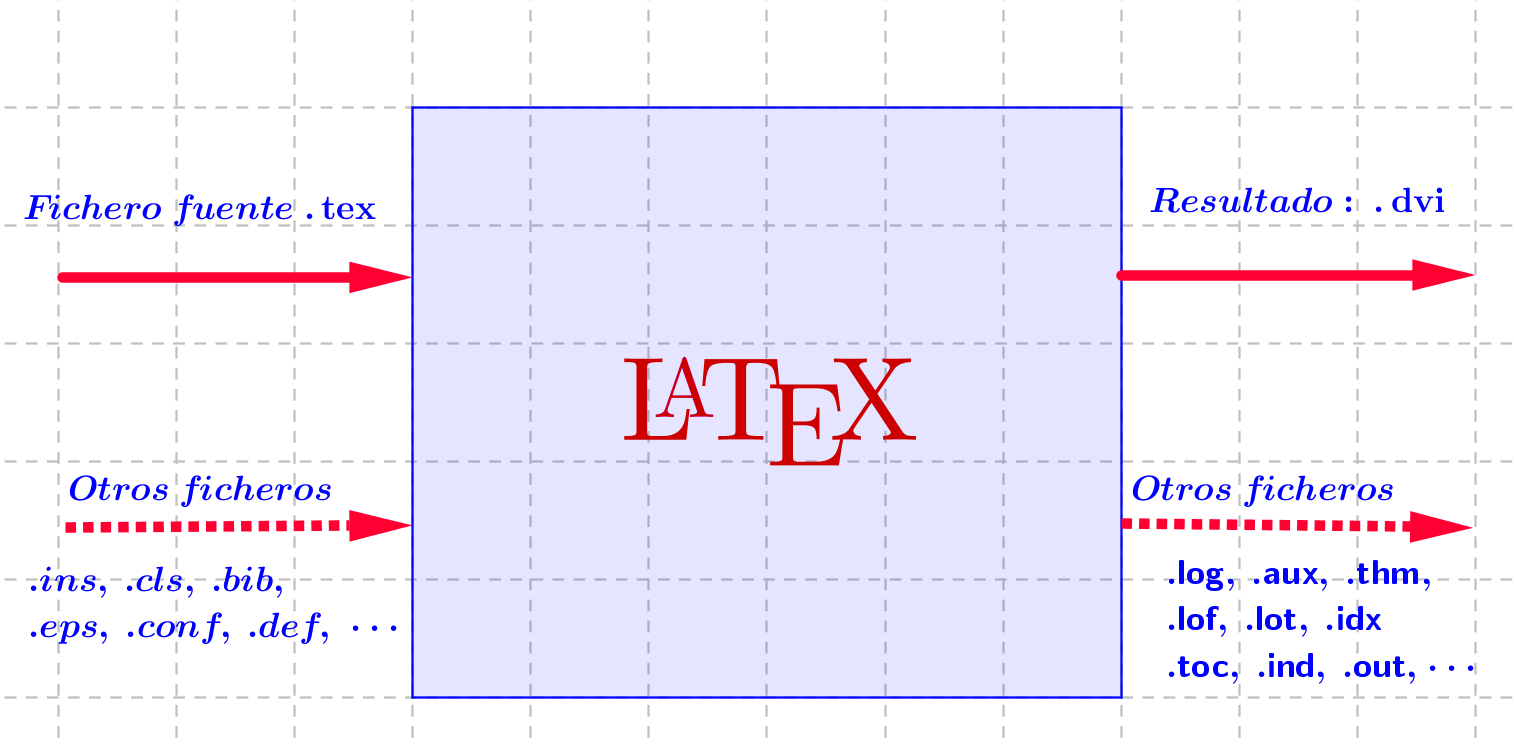
\includegraphics[scale=0.6]{diagrama.png}
\end{figure}


\chapter{tercer}
\chaptertoc 
\begin{objetivos}
\begin{lista}
\item Comprender el esquema básico de funcionamiento de \TeX\, y \LaTeX .
\item Conocer las diferentes salidas que produce \LaTeX.
\item Conocer las diferentes herramientas que intecactuan con \LaTeX.
\item Aprender a instalar \LaTeX\, en diferentes sistemas.
\end{lista}
\end{objetivos}
\section{Reglas generales}

\begin{description}
\item[$\clubsuit$] Usar espacios para separar palabras.

\item Un espacio vale igual que mil.

\begin{description}
\item[$\clubsuit$] Los fines de linea sencillos no valen.

\item[$\clubsuit$] Usar líneas vac\'{\i}as para separar p\'{a}rrafos.
\end{description}
\end{description}

Una linea vac\'{\i}a vale igual que mil.

\begin{description}
\item
\begin{description}
\item[$\clubsuit$] El espaciado y las sangr\'{\i}as son trabajo de
\end{description}

\item LATEX, y lo sabe hacer muy bien.

\begin{description}
\item[$\clubsuit$] No forzar espacios ni cortes de l\'{\i}nea.
\end{description}
\end{description}

\subsection{Ejemplo 1}
\begin{verbatim}
\begin{document}
\maketitle Este es el primer párrafo ,
y esta sigue
siendo par te del primer p árrafo
 Este ya es e l segundo párrafo .
%y esto es un comentario
Aquí puedes e s c r i b i r más .
\ end{ document }

\end{verbatim}

\subsection{Ejemplo 2}
\begin{verbatim}

\begin{document}
\maketitle Este es un ejemplo con un
p á r ra fo m\'{a}s grande
que , por c i e r t o , tambi \'{e}n
es mucho m\'{a}s i n te re sa
n te . Recuerda que un p\'{a} r ra fo
debe expresar una idea
completa y coherente . Justo como este
 p \'{a} r ra fo que nos ha
servido como un ejemplo genial . Observa
que los p \'{a} r ra fo s
en \ LaTeX { } forman l a unidad
e s t r u c t u r a l m\'{a}s
peque~na dent ro de los documentos .
 Recuerda que es tu responsabilidad
  e l contenido de estos
párrafos , y de \ LaTeX { } e l
que se vean boni tos . \ end{ document }
\end{verbatim}

\subsection{Acentos}

La opci\'{o}n activeacute de babel permite

usar acentos cortos: \'{a}, \'{a}, \'{a}, \~{n}, etc.

Los acentos cortos no funcionan en el

pre\'{a}mbulo, all\'{\i} hay que usar acentos largos:

\'{a}
%TCIMACRO{\TEXTsymbol{\backslash}}%
%BeginExpansion
$\backslash$%
%EndExpansion
\'a \'{o}
%TCIMACRO{\TEXTsymbol{\backslash}}%
%BeginExpansion
$\backslash$%
%EndExpansion
\'o

\'{e}
%TCIMACRO{\TEXTsymbol{\backslash}}%
%BeginExpansion
$\backslash$%
%EndExpansion
\'e \'{u}
%TCIMACRO{\TEXTsymbol{\backslash}}%
%BeginExpansion
$\backslash$%
%EndExpansion
\'u

\'{\i}
%TCIMACRO{\TEXTsymbol{\backslash}}%
%BeginExpansion
$\backslash$%
%EndExpansion
'\{%
%TCIMACRO{\TEXTsymbol{\backslash}}%
%BeginExpansion
$\backslash$%
%EndExpansion
i\} \~{n}
%TCIMACRO{\TEXTsymbol{\backslash}}%
%BeginExpansion
$\backslash$%
%EndExpansion%
%TCIMACRO{\U{2dc}}%
%BeginExpansion
\protect\rule{0.1in}{0.1in}
%EndExpansion
n

\textquestiondown Por qu\'{e} no usar directamente los caracteres

acentuados en mi c\'{o}digo de \LaTeX?

Tambi\'{e}n podemos usar el paquete inputenc con la opci\'{o}n latin1

\subsection{F\'{o}rmulas en l\'{\i}neas}

\begin{description}
\item[$\blacksquare$] Los signos \$ \$ son para indicar el contenido
\end{description}

matem\'{a}tico.

\begin{description}
\item[$\blacksquare$] Todo el contenido matem\'{a}tico (y s\'{o}lo el
\end{description}

contenido matem\'{a}tico) debe de ser marcado.

\begin{description}
\item[$\blacksquare$] No usar el contenido matem\'{a}tico para poner
\end{description}

it\'{a}licas.

\begin{description}
\item[$\blacksquare$] Y no usar comandos de formato para marcar
\end{description}

contenido matem\'{a}tico.

\begin{description}
\item[$\blacksquare$] Pensar en el contenido, \textexclamdown no en el formato!.
\end{description}

\subsection{Mas ejemplos}

\begin{example}
Haciendo salvedad de ((efectos es-peciales)),
para escribir un texto
normal en \TeX \,basta con teclear
exactamente el texto que se de-
sea. El cajista (\TeX) se ocupa de
formar y ajustar las l\'{\i}neas. Para
separar las palabras se emplean
espacios en blanco o ((retornos de
carro)) (nueva l\'{\i}nea). El n\'{u}mero
de espacios en blanco no impor-
ta: uno es igual que                100.
\end{example}
\subsection{Tipos de documentos}
\begin{description}
\item[$\blacksquare$] Clase del documento
\item (\lstinline+\documentclass[...]{clase}+):

\item[$\bigstar$]  article: art\'{\i}culos, trabajos, : : :

\item[$\bigstar$]  letter: cartas

\item[$\bigstar$]  report, book: documentos m\'{a}s largos, con cap\'{\i}tulos

\item[$\bigstar$]  slides: presentaciones (transparencias)
\item[$\blacksquare$] Par\'{a}metros opcionales (\lstinline+\documentclass[opciones]{...}+):
\end{description}

10pt, 11pt, 12pt: tama\~{n}os o tipos

letterpaper, a4paper:  tama\~{n}o o papel

twocolumn: dos columnas


\chapter{\LaTeX\, con LYX}
%\chapter{Mas}



\section{Salto de l'inea y de p'agina}

\subsection{P'arrafos justificados}

Normalmente los libros se suelen componer con todos los renglones del
mismo tama~no. \LaTeX{} inserta los saltos de l'inea y los espacios
entre las palabras optimizando el contenido de los p'arrafos enteros.
Si es necesario, tambi'en introduce guiones, dividiendo las palabras
que no encajen bien al final de los renglones. El modo de componer los
p'arrafos depende de la clase de documento. Normalmente se introduce
una sangr'ia horizontal en la primera l'inea de un p'arrafo y no se
introduce espacio adicional entre cada dos p'arrafos. Para m'as
informaci'on v'ease el apartado~\ref{parsp}.

En casos especiales se podr'ia ordenar a \LaTeX{} que introduzca un
salto de l'inea.

\begin{command}
\ci{\bs} o \ci{newline}
\end{command}
\noindent comienza una l'inea nueva sin comenzar un p'arrafo nuevo.

\begin{command}
\ci{\bs*}
\end{command}
\noindent adem'as proh'ibe que se produzca un salto de p'agina tras el
salto de l'inea.

\begin{command}
\ci{newpage}
\end{command}
\noindent comienza una p'agina nueva.
\pagebreak

\begin{command}
\ci{linebreak}\verb|[|\emph{n}\verb|]|,
\ci{nolinebreak}\verb|[|\emph{n}\verb|]|,
\ci{pagebreak}\verb|[|\emph{n}\verb|]| and
\ci{nopagebreak}\verb|[|\emph{n}\verb|]|
\end{command}
\noindent hacen lo que indican sus nombres: salto de l'inea,
ning'un salto de l'inea, salto de p'agina y ning'un salto de
p'agina. Adem'as le permite al autor el influir sobre sus acciones
a trav'es del argumento opcional \emph{n}. Se puede establecer a
un valor entre cero y cuatro. Al poner \emph{n} menor de 4 se le
deja a \LaTeX{} la posibilidad de ignorar la orden si el resultado
resulta muy malo.

\LaTeX{} siempre intenta realizar los saltos de l'inea lo mejor
posible. Si no puede encontrar ninguna posibilidad satisfactoria para
producir los bordes de los p'arrafos totalmente rectos, cumpliendo con
las reglas impuestas, entonces dejar'a un rengl'on demasiado largo.
En este caso \LaTeX{} producir'a el correspondiente mensaje de
advertencia (``\wni{overfull box}'') mientras procesa el fichero de
entrada. Esto sucede en especial si no se encuentra un lugar apropiado
para introducir un gui'on entre las s'ilabas. Si se introduce la orden
\ci{sloppy}, \LaTeX{} ser'a menos severo en sus exigencias y evita
tales renglones con longitudes mayores, aumentando la separaci'on
entre las palabras ---si bien el resultado final no es de lo mejor---.
En este caso se dan mensajes de advertencia (``\wni{underfull
  hbox}''). El resultado suele ser perfectamente aceptable la mayor'ia
de las veces. La orden \ci{fussy} act'ua en sentido contrario. Esto
podr'ia hacerlo en caso que desee ver a \LaTeX{} quejarse en todos los
sitios.


\subsection{Silabeo} \label{hyph}

\LaTeX{} silabea las palabras cuando resulta necesario. Si el
algoritmo de silabeo no produce los resultados correctos, entonces se
puede remediar esta situaci'on con 'ordenes como las que presentamos a
continuaci'on. Esto suele ser especialmente necesario en palabras
compuestas o de idiomas extranjeros.

La instrucci'on
\begin{command}
\ci{hyphenation}\verb|{|\emph{lista de palabras}\verb|}|
\end{command}
\noindent da lugar a que las palabras mencionadas en ella se puedan
dividir en cualquier momento en, y s'olo en, los lugares indicados con
``\verb|-|''\@. Esta orden deber'ia aparecer en el pre'ambulo del
fichero de entrada y deber'ia contener solamente palabras construidas
sin caracteres especiales.
%%% Alguna idea de la definici'on de ``letras normales''???
%%% Es lo que aparece en el documento en ingl'es...
No se hacen distinciones entre las letras may'usculas y min'usculas
de las palabras a las que se refiera esta orden. El ejemplo siguiente
permitir'a localizar las s'ilabas de ``fichero'' y ``Fichero'' del
mismo modo, e impedir'a que en las palabras ``FORTRAN'', ``Fortran'' y
``fortran'' se introduzcan guiones. No se permiten caracteres con
acentos o s'imbolos en el argumento.
%%% Pues podr'ian plante'arselo por lo menos... :-)

Ejemplo:
\begin{code}
\verb|\hyphenation{FORTRAN fi-che-ro}|
\end{code}

Dentro de una palabra, la instrucci'on \ci{-} establece un sitio donde
colocar un gui'on si fuese necesario. Adem'as, 'estos se convierten en
los 'unicos lugares donde se permite introducir los guiones en esta
palabra. Esta instrucci'on es especialmente 'util para las palabras
que contienten caracteres especiales (como, por ej., los caracteres
con acento ortogr'afico), ya que \LaTeX{} no silabea de modo
autom'atico las palabras que contienen estos caracteres.
%\footnote{A no ser que est'e usando los nuevos
%\wi{tipos DC}}.

\begin{example}
Me parece que esto es: su\-per\-%
ca\-li\-fra\-gi\-lis\-ti\-co\-%
ex\-pia\-li\-do\-so
\end{example}

Tambi'en se pueden se pueden mantener varias palabras en el mismo
rengl'on con la orden
\begin{command}
\ci{mbox}\verb|{|\emph{texto}\verb|}|
\end{command}
\noindent Hace que su argumento se mantenga siempre unido bajo cualquier
circunstancia, o sea, que no se puede dividir.

\begin{example}
Dentro de poco tendr'e otro tel'efono.
Ser'a el \mbox{(0203) 3783-225}.

El par'ametro \mbox{\emph{nombre
de fichero}} debe contener el nombre
del fichero.
\end{example}


\subsection{Guiones y rayas}

\LaTeX{} reconoce cuatro tipos de \wi{guiones}. Para tener acceso a
tres de 'estos se pone una cantidad diferente de guiones consecutivos.
El cuarto tipo es el signo matem'atico `menos':
\index{-}%
\index{--}%
\index{---}%
\index{-@$-$}%
\index{matem'atico!menos}%

\begin{example}
psico-terap'eutico \\
10--18~horas \\
Madrid -- Barcelona \\
?`S'i? ---dijo ella--- \\
0, 1 y $-1$
\end{example}

% En ingl'es, los nombres de estos guiones son:
% \texttt{-} \wi{hyphen}, \texttt{--} \wi{en-dash},
% \texttt{---} \wi{em-dash} y \verb|$-$| \wi{signo menos}.

\subsection{Puntos suspensivos (`\ldots')}

En una m'aquina de escribir, tanto para la \wi{coma} como para el
\wi{punto} se les da el mismo espaciado que a cualquier otro
car'acter. En la impresi'on de libros, estos caracteres s'olo ocupan
un peque~no espacio y se colocan muy pr'oximos al car'acter que les
precede. Por esto, los ``puntos suspensivos'' no se pueden introducir
con tres puntos normales, ya que no tendr'ian el espaciado correcto.
Para estos puntos existe una instrucci'on especial llamada
\begin{command}
\ci{ldots}
\end{command}
\index{...@\ldots}
\begin{example}
No as'i ... sino as'i:\\
New York, Tokyo, Budapest\ldots
\end{example}

\subsection{Ligaduras}

Algunas combinaciones de letras no se componen con las distintas
letras que la forman, sino que, de hecho, se usan s'imbolos
especiales.
\begin{code}
{\large ff fi fl ffi\ldots}\quad
en lugar de\quad {\large f{}f f{}i f{}l f{}f{}i \ldots}
\end{code}
Estas \wi{ligaduras} se pueden evitar intercalando \ci{mbox}\verb|{}|
entre el par letras en cuesti'on.





\section{Distancias entre palabras}

Para conseguir un margen derecho recto en la salida, \LaTeX{}
introduce cantidades variables de espacios entre las palabras. Al
final de una oraci'on, introduce unos espacios algo mayores que
favorecen la legibilidad del texto. \LaTeX{} presupone que las frases
acaban con puntos, signos de interrogaci'on y de admiraci'on. Si hay
un punto tras una letra may'uscula, entonces esto no se considera el
fin de una oraci'on ya que los puntos tras las letras may'usculas
normalmente se utilizan para abreviaturas.

El autor debe indicar cualquier excepci'on a estas reglas. Una
\emph{barra invertida} \verb|\| antes de un espacio en blanco produce
un espacio en blanco que no se ensanchar'a. Un car'acter de
tilde~`\verb|~|'\ genera un espacio que no se puede ensanchar y en el
que no se puede producir ning'un cambio de rengl'on. Si antes de un
punto aparece la instrucci'on \verb|\@|, significa que este punto
acaba una oraci'on, aunque se encuentre tras una letra may'uscula.
\cih{"@} \index{~@\verb.~.} \index{tilde@tilde (\verb.~.)} \index{.!
  espacio tras}

\begin{example}
En la fig.\ 1 del cap.\ 1\dots \\
El Dr.~L'opez se encuentra \\
con D~na.~P'erez. \\
\dots\ 5~m de ancho. \\
Necesito vitamina~C\@. ?`Y t'u?
\end{example}

Este tratamiento especial para los espacios al final de las oraciones
se puede evitar con la instrucci'on
\begin{command}
\ci{frenchspacing}
\end{command}
\noindent que le indica a \LaTeX{} que \emph{no} introduzca m'as
espacios tras un punto que tras cualquier otro car'acter. Esto es muy
com'un en diversos idiomas, como es el caso del espa~nol. En este caso
la instrucci'on \verb|\@| no es necesaria.




\section{Referencias cruzadas}

En los libros, informes y art'iculos existen, a menudo,
\wi{referencias cruzadas} a figuras, tablas y segmentos especiales de
texto que se hayan en otros lugares del documento. \LaTeX{}
proporciona las siguientes instrucciones para producir referencias
cruzadas:
\begin{command}
  \ci{label}\verb|{|\emph{marcador}\verb|}|,
  \ci{ref}\verb|{|\emph{marcador}\verb|}| y
  \ci{pageref}\verb|{|\emph{marcador}\verb|}|
\end{command}
\noindent donde \emph{marcador} es un identificador elegido por el
usuario. \LaTeX{} reemplaza \verb|\ref| por el n'umero del apartado,
subapartado, figura, tabla o teorema donde se introdujo la
instrucci'on \verb|\label| correspondiente. La orden \verb|\pageref|
imprime el n'umero de p'agina donde se produce la orden \verb|\label|
con igual argumento. Aqu'i tambi'en se utilizan los n'umeros del
procesamiento anterior.

\begin{example}
Una referencia a este subapartado
\label{sec:este} aparecer'ia como:

``vea el apartado~\ref{sec:este} en
la p'agina~\pageref{sec:este}.''
\end{example}

\section{Notas a pie de p'agina}

Con la instrucci'on
\begin{command}
\ci{footnote}\verb|{|\emph{texto de la nota al pie}\verb|}|
\end{command}
\noindent se imprimir'a una nota en el pie de la p'agina actual.

\begin{example}
Las notas a pie de p'agina%
\footnote{Esta es una nota a pie
de p'agina} son utilizadas con
frecuencia por la gente que usa
\LaTeX.
\end{example}

Tambi'en existe una variante de esta instrucci'on, que es
\begin{command}
\ci{footnote}\verb|[|\emph{n'umero}\verb|]{|\emph{texto de la nota al
    pie}\verb|}|
\end{command}
De esta forma para la nota al pie correspondiente se emplear'a para el
marcador el \emph{n'umero} que se ha indicado en vez del valor del
contador de notas al pie. Esta variante \emph{s'olo} se puede emplear
dentro de los p'arrafos.

\section{Palabras resaltadas}

En los escritos a m'aquina, para resaltar determinados segmentos de
texto 'estos se $\underline{\mathrm{subrayan}}$. En los libros
impresos estas palabras se \emph{resaltan} o se \emph{destacan}. La
orden con la que se cambia a un tipo de letra \emph{resaltado} es
\begin{command}
\ci{emph}\verb|{|\emph{texto}\verb|}|
\end{command}
\noindent Su argumento es el texto que se debe \wi{resaltar}.

\begin{example}
\emph{Si est'a empleando
\emph{resalte} en un texto
ya resaltado, entonces \LaTeX{}
utiliza \emph{redonda} para volver
a resaltar texto.}
\end{example}


\section{Entornos} \label{env}

Para componer textos con un prop'osito especial \LaTeX{} define muchos
tipos de \wi{entornos} para toda clase de dise~nos:
\begin{command}
\ci{begin}\verb|{|\emph{nombre}\verb|}|\quad
   \emph{texto}\quad
\ci{end}\verb|{|\emph{nombre}\verb|}|
\end{command}
\noindent donde \emph{nombre} es el nombre del entorno. Los entornos
son ``grupos'' o ``agrupaciones''. Tambi'en se puede cambiar a un
nuevo entorno dentro de otro, en cuyo caso debe tenerse cuidado con la
secuencia:
\begin{code}
\verb|\begin{aaa}...\begin{bbb}...\end{bbb}...\end{aaa}|
\end{code}

En los apartados siguientes se explican todos los entornos importantes.

\subsection{Listas y descripciones (\texttt{itemize},
  \texttt{enumerate}, \texttt{description})}

El entorno \ei{itemize} es adecuado para las listas sencillas, el
entorno \ei{enumerate} para relaciones numeradas y el entorno
\ei{description} para descripciones.\cih{item}

\begin{example}
\begin{enumerate}
\item Puede mezclar los entornos
de listas a su gusto:
\begin{itemize}
\item Pero podr'ia comenzar a
perecer inc'omodo.
\item Si abusa de ellas.
\end{itemize}
\item Por lo tanto, recuerde:
\begin{description}
\item[Lo innecesario] no va a
resultar adecuado porque
lo coloque en una lista.
\item[Lo adecuado,] sin embargo,
se puede presentar agradablemente
en una lista.
\end{description}
\end{enumerate}
\end{example}

\subsection{Justificaciones y centrado (\texttt{flushleft},
            \texttt{flushright}, \texttt{center})}

Los entornos \ei{flushleft} y \ei{flushright} producen p'arrafos
justificados a la izquierda y a la derecha (sin nivelaci'on de
bordes).%
\index{justificado a la izquierda}\index{justificado a la derecha} El
entorno \ei{center} genera texto centrado. Si no se introduce \ci{\bs}
para dividir los renglones, entonces \LaTeX{} lo har'a
autom'aticamente.

\begin{example}
\begin{flushleft}
Este texto est'a\\ justificado a
la izquierda. \LaTeX{} no intenta
forzar que todas las l'ineas
tengan longitud.
\end{flushleft}
\end{example}

\begin{example}
\begin{flushright}
Este texto est'a\\ justificado a
la derecha. \LaTeX{} no intenta
forzar que todas las l'ineas
tengan igual longitud.
\end{flushright}
\end{example}

\begin{example}
\begin{center}
En el centro\\de la tierra
\end{center}
\end{example}

\subsection{Citas (\texttt{quote}, \texttt{quotation}, \texttt{verse})}

El entorno \ei{quote} sirve para citas peque~nas, ejemplos y para
resaltar oraciones.
\begin{example}
Una regla de oro en tipograf'ia
para el largo de los renglones
dice:
\begin{quote}
Ning'un rengl'on debe contener
m'as de 66~letras.
\end{quote}
Por esto se suelen utilizar varias
columnas en los peri'odicos.
\end{example}
% Curioso lo que hace el ``66~letras'' en el primer rengl'on. Hay un
% modo de indicar preferencias entre la divisi'on de ``debe'' y
% ``66~letras''?


Hay dos entornos muy parecidos: el entorno \ei{quotation} y el entorno
\ei{verse}. El entorno \texttt{quotation} es adecuado para citas
mayores que consten de varios p'arrafos. El entorno \texttt{verse} es
apropiado para poemas en los que la separaci'on de los renglones es
esencial. Los versos (los renglones) se dividen con \ci{\bs} y las
estrofas con renglones en blanco.

\begin{example}
\begin{flushleft}
\begin{verse}
Soberano gofio en polvo,\\
sustento de mi barriga,\\
el d'ia que no te como\\
para m'i no hay alegr'ia.
\end{verse}
\end{flushleft}
\end{example}

\subsection{Edici'on directa (\texttt{verbatim}, \texttt{verb})}

El texto que se encuentre entre \verb|\begin{|\ei{verbatim}\verb|}| y
  \verb|\end{verbatim}| aparecer'a tal como se ha introducido, como si
se hubiese escrito con una m'aquina de escribir, con todos los espacios
en blanco y cambios de l'inea y sin interpretaci'on de las
instrucciones de \LaTeX.

Dentro de un p'arrafo se puede lograr el mismo efecto con
\begin{command}
\ci{verb}\verb|+|\emph{text}\verb|+|
\end{command}

\noindent El \verb|+| s'olo es un ejemplo de car'acter delimitador. Se
puede usar cualquier car'acter excepto las letras, \verb|*| o
caracteres en blanco.

\begin{example}
La instrucci'on \verb|\ldots|%
\ldots

\begin{verbatim}
10 PRINT "HELLO WORLD ";
20 GOTO 10
\end{verbatim}
\end{example}

\begin{example}
\begin{verbatim*}
La version con estrella del
entorno          verbatim
destaca los espacios     en
el  texto
\end{verbatim*}
\end{example}

La instrucci'on \ci{verb} se puede usar, del mismo modo, con un
asterisco:
\begin{example}
\verb*|de esta   manera :-) |
\end{example}

El entorno \texttt{verbatim} y la instrucci'on \verb|\verb| no pueden
utilizarse como par'ametros de otras instrucciones.


\subsection{Estadillos (\texttt{tabular})}

El entorno \ei{tabular} sirve para crear \wi{estadillos}, con l'ineas
horizontales y verticales seg'un se desee. \LaTeX{} determina el ancho
de las columnas de modo autom'atico.

El argumento \emph{especificaciones del estadillo} de la instrucci'on
\begin{command}
\verb|\begin{tabular}{|\emph{especificaciones del estadillo}\verb|}|
\end{command}
\noindent define el dise~no del estadillo. Utilice \texttt{l} para una
columna con texto justificado a la izquierda, \texttt{r} para
justificar el texto a la derecha, \texttt{c} para texto centrado,
\verb|p{|\emph{ancho}\verb|}| para una columna que contenga texto con
saltos de l'inea, y \verb.|. para una l'inea vertical.


Dentro de un entorno \texttt{tabular}, \verb|&| salta a la pr'oxima
columna, \ci{\bs} separa los renglones y \ci{hline} introduce una
l'inea horizontal.
\index{"|@ \verb."|.}
\begin{example}
\begin{tabular}{|r|l|}
\hline
7C0 & hexadecimal \\
3700 & octal \\
11111000000 & binario \\
\hline \hline
1984 & decimal \\
\hline
\end{tabular}
\end{example}

\begin{example}
\begin{tabular}{|p{4.7cm}|}
\hline
Bienvenido al p'arrafo del Sr.\
Caj'on. Esperamos que disfrute
del espect'aculo.\\
\hline
\end{tabular}

\end{example}

Con la construcci'on \verb|@{...}| se puede especificar el separador
de columnas. Esta construcci'on elimina el espacio entre columnas y lo
reemplaza con lo que se haya introducido entre los par'entesis. Un uso
muy frecuente de esta construcci'on se explica m'as adelante con el
problema de la alineaci'on de la coma decimal. Otro uso posible es
para eliminar el espacio que antecede y precede a los renglones de una
tabla con \verb|@{}|.

\begin{example}
\begin{tabular}{@{} l @{}}
\hline
ning'un espacio a la izquierda
ni derecha\\\hline
\end{tabular}
\end{example}
\begin{example}
\begin{tabular}{l}
\hline
espacios a la izquierda
y a la derecha\\
\hline
\end{tabular}
\end{example}

\index{alineaci'on decimal} Ya que no hay ning'un mecanismo
incorporado para alinear columnas num'ericas sobre la coma decimal
\footnote{Si se halla instalado el conjunto `tools'\ en su sistema,
  eche un vistazo al paquete \pai{dcolumn}.}, podr'iamos ``imitarlo''
usando dos columnas: un entero alineado a la derecha y luego los
decimales a la izquierda. La instrucci'on \verb|@{,}| en el argumento
de \verb|\begin{tabular}| reemplaza el espacio normal entre columnas
  con una ``,'', dando la apariencia de una 'unica columna justificada
  por la coma decimal. !`No se olvide de reemplazar la coma decimal en
  sus n'umeros con un separador de columna (\verb|&|)! Se puede
  colocar una etiqueta sobre nuestra ``columna'' num'erica empleando
  la instrucci'on \ci{multicolumn}.

\begin{example}
\begin{tabular}{c r @{,} l}
Expresi'on en pi       &
\multicolumn{2}{c}{Valor} \\
\hline
$\pi$               & 3&1416  \\
$\pi^{\pi}$         & 36&46   \\
$(\pi^{\pi})^{\pi}$ & 80662&7 \\
\end{tabular}
\end{example}

\section{Elementos flotantes}

Hoy en d'ia, la mayor'ia de las publicaciones contienen muchas
ilustraciones y tablas. Estos elementos necesitan un tratamiento
especial porque no se pueden cortar entre p'aginas. Un m'etodo podr'ia
ser comenzando una p'agina nueva cada vez que una ilustraci'on o una
tabla sea demasiado larga para caber en la p'agina actual. Este
enfoque deja p'aginas parcialmente vac'ias, lo que resulta poco
est'etico.

La soluci'on a este problema es hacer que cualquier ilustraci'on o
tabla que no quepa en la p'agina actual `flote'\ hasta una p'agina
posterior mientras se rellena la p'agina actual con el texto del
documento.

\LaTeX{} ofrece dos entornos para los \wi{elementos flotantes}. Uno
 para las tablas y otro para las ilustraciones. Para aprovechar
 completamente estos dos entornos es importante entender
 aproximadamente c'omo maneja \LaTeX{} estos objetos flotantes
 internamente. Si no, los objetos flotantes se pueden convertir en una
 fuente de frustaciones porque \LaTeX{} nunca los pone donde Vd.\
 quiere que vayan.

\bigskip
Primeramente, echemos un vistazo a las instrucciones que \LaTeX{}
proporciona para objetos flotantes.

Cualquier cosa que se incluya en un entorno \ei{figure} o \ei{table}
ser'a tratado como materia flotante. Ambos entornos flotantes
proporcionan un par'ametro opcional
\begin{command}
\verb|\begin{figure}[|\emph{designador de colocado}\verb|]| o\\
\verb|\begin{table}[|\emph{designador de colocado}\verb|]|
\end{command}
\noindent llamado el \emph{designador de colocado}. Este par'ametro se
emplea para indicarle a \LaTeX{} los lugares donde se permite que vaya
colocado el objeto flotante. Un \emph{designador de colocado} se
construye con una cadena de \emph{permisos de colocaci'on flotante}.
V'ease la tabla~\ref{tab:permiss}.

\begin{table}[!bp]
\caption{Permisos de colocaci'on flotante}\label{tab:permiss}
\noindent \begin{minipage}{\textwidth}
\medskip
\begin{center}
\begin{tabular}{@{}cp{10cm}@{}}
  Designador&Permiso para colocar el objeto flotante\ldots\\ \hline
  \rule{0pt}{1.05em}
\texttt{h} & aqu'i (\emph{here}), muy pr'oximo al
  lugar en el texto donde se ha introducido. Es 'util, principalmente,
  para objetos flotantes peque~nos.\\[0.3ex]
\texttt{t} & en la parte superior de una p'agina (\emph{top}).\\[0.3ex]
\texttt{b} & en la parte inferior de una p'agina
  (\emph{bottom}).\\[0.3ex]
\texttt{p} & en una \emph{p'agina} especial que s'olo contenga
  elementos flotantes.\\[0.3ex]
\texttt{!} & sin considerar la mayor'ia de los par'ametros
  internos\footnote{Como el n'umero m'aximo de elementos flotantes un
  una p'agina.} que impedir'ian a este objeto flotante que se colocase.
\end{tabular}
\end{center}
\end{minipage}
\end{table}

\pagebreak[3]
Una tabla se podr'ia comenzar con, por ejemplo, la siguiente l'inea:
\begin{code}
\verb|\begin{table}[!hbp]|
\end{code}
\noindent El \wi{designador de colocado} \verb|[!hbp]| le permite a
\LaTeX{} colocar la tabla justamente aqu'i (\texttt{h}) o al final
 (\texttt{b}) de alguna p'agina o en alguna p'agina especial para
 elementos flotantes, y en cualquier parte si no queda tan bien
 (\texttt{!}). Si no se da ning'un designador de colocado, entonces
 las clases normalizadas sobreentienden \verb|[tbp]|.

 \LaTeX{} colocar'a todos los objetos flotantes que encuentra seg'un
 los de\-sig\-na\-do\-res de colocado que haya indicado el autor. Si
 un objeto flotante no se puede colocar en la p'agina actual entonces
 se aplaza su colocaci'on, para lo cual se introduce en una
 cola\footnote{Son de tipo \emph{fifo}: lo que se introdujo primero es
   lo primero en extraerse.} de \emph{tablas} o \emph{figuras}
 (ilustraciones).  Cuando se comienza una nueva p'agina, lo primero
 que hace \LaTeX{} es confirmar si se puede construir una p'agina
 especial con los objetos flotantes que se hayan en las colas. Si no
 es posible, entonces se trata el primer objeto que se encuentra en
 las colas como si lo acab'asemos de introducir. Entonces \LaTeX{}
 vuelve a intentar colocar el objeto seg'un sus designadores de
 colocado (eso s'i, sin tener en cuenta la opci'on `\verb|h|',\ que ya
 no es posible). Cualquier objeto flotante nuevo que aparezca en el
 texto se introduce en la cola correspondiente. \LaTeX{} mantiene
 estrictamente el orden original de apariciones de cada tipo de objeto
 flotante.

Esta es la raz'on por la que una ilustraci'on que no se puede colocar
desplaza al resto de las figuras al final del documento. Por lo tanto:


\begin{quote}
  Si \LaTeX{} no coloca los objetos flotantes como esperaba, suele
  deberse 'unicamente a un objeto flotante que est'a atascando una de
  las dos colas de objetos flotantes.
\end{quote}

\bigskip
\noindent Adem'as, existen algunas cosas m'as que se deben indicar
sobre los entornos \ei{table} y \ei{figure}. Con la instrucci'on
\begin{command}
\ci{caption}\verb|{|\emph{texto de t'itulo}\verb|}|
\end{command}
\noindent se puede definir un t'itulo para el objeto flotante. \LaTeX{}
le a~nadir'a la cadena ``Figura'' o ``Tabla'' y un n'umero de secuencia.


Las dos instrucciones
\begin{command}
\ci{listoffigures} y \ci{listoftables}
\end{command}
\noindent funcionan de modo an'alogo a la orden
\verb|\tableofcontents|, imprimiendo un 'indice de figuras o de tablas
respectivamente. En estas listas se repetir'an los t'itulos
completos. Si Vd.\ tiende a utilizar t'itulos largos, deber'ia tener
una versi'on de estos t'itulos m'as cortos para introducirlos en estos
'indices. Esto se consigue dando la versi'on corta entre corchetes
tras la orden \verb|\caption|.
\begin{code}
\verb|\caption[Corto]{LLLLLaaaaaaaaarrrrrrrrgggggooooooo}|
\end{code}

Con \verb|\label| y \verb|\ref| se pueden crear referencias a un
objeto flotante dentro del texto.

El siguiente ejemplo dibuja un cuadrado y lo inserta en el
documento. Podr'ia utilizar esto si desea reservar espacios para
im'agenes que vaya a pegar en el documento acabado.

\begin{example}
La ilustraci'on~\ref{blanco} es un ejemplo del Pop-Art.
\begin{figure}[!hbp]
\makebox[\textwidth]{\framebox[5cm]{\rule{0pt}{5cm}}}
\caption{$5\times 5$ cent'imetros} \label{blanco}
\end{figure}
\end{example}

\noindent En el ejemplo anterior\footnote{suponiendo que la cola de
  figuras est'e vac'ia.} \LaTeX{} intentar'a \emph{por todos los
  medios}~(\texttt{!}) colocar la ilustraci'on exactamente
\emph{aqu'i}~(\texttt{h}). Si no puede, intentar'a colocarla en la
\emph{parte inferior}~(\texttt{b}) de la p'agina. Si no consigue
colocar esta figura en la p'agina actual, determina si es posible
crear una p'agina (\verb|p|) con elementos flotantes exclusivamente
que contenga esta ilustraci'on y algunas tablas que pudieran haber en
la cola de tablas. Si no hay material suficiente para una p'agina
especial de objetos flotante, entonces \LaTeX{} comienza una p'agina
nueva y otra vez trata la figura como si acabase de aparecer en el
texto.

Bajo determinadas condiciones podr'ia ser necesario emplear la orden
\begin{command}
\ci{clearpage}
\end{command}
\noindent Le ordena a \LaTeX{} que coloque \emph{inmediatamente} todos
los objetos flotantes que se hallen en las colas y despu'es comenzar
una p'agina nueva.

M'as adelante veremos c'omo incluir im'agenes en formato PostScript en
sus documentos de \LaTeXe.


\section{A~nadiendo instrucciones y entornos nuevos}

En el primer cap'itulo se explic'o que \LaTeX{} necesita informaci'on
sobre la estructura l'ogica del texto para elegir el formato
adecuado. Este es un concepto muy bien cuidado. Pero en la pr'actica
solemos chocar con las limitaciones que esto nos impone, ya que
\LaTeX{} simplemente no tiene el entorno especializado o la orden que
deseamos para un prop'osito espec'ifico.

Una soluci'on es emplear varias 'ordenes de \LaTeX{} para producir el
dise~no que se tiene en mente. Si tiene que hacer esto una vez, no hay
ning'un problema. Pero si esto sucede repetidamente, entonces lleva
mucho tiempo. Si alguna vez desease cambiar el formato tendr'ia que
revisar el fichero de entrada entero y editar todos los elementos en
cuesti'on.

Para resolver este problema, \LaTeX{} le permite definir sus propias
instrucciones y entornos.

\subsection{Instrucciones nuevas}

Para a~nadir sus propias instrucciones utilice la orden
\begin{command}
\ci{newcommand}\verb|{|%
   \emph{nombre}\verb|}[|\emph{num}\verb|]{|\emph{definici'on}\verb|}|
\end{command}
\noindent B'asicamente, la instrucci'on necesita dos argumentos: el
\emph{nombre} de la instrucci'on que quiere crear y la
\emph{definici'on} de la instrucci'on. El argumento entre corchetes
\emph{num} es opcional. Puede usarlo para crear 'ordenes nuevas que
tomen hasta 9 argumentos.

Los dos ejemplos siguientes deber'ian ayudarle a captar la idea. El
primer ejemplo define una instrucci'on nueva llamada
\verb|\udl|. Esta es una forma abreviada de introducir ``Una
Descripci'on de \LaTeXe''. Una orden como 'esta ser'ia muy 'util si
tuviese que escribir el t'itulo de este documento una y otra vez.

\begin{example}
\newcommand{\udl}
    {Una Descripci'on de \LaTeXe}
% en el cuerpo del documento :
``\udl'' \ldots{} ``\udl''
\end{example}

El siguiente ejemplo ilustra c'omo usar el argumento \emph{num}. La
secuencia \verb|#1| encuentra un sustituto en el argumento que
especifique. Si quisiera m'as de un argumento, emplee \verb|#2| y as'i
sucesivamente.

\begin{example}
\newcommand{\txsit}[1]
    {Una Descripci'on \emph{#1}
     Peque~na de \LaTeXe}
% en el cuerpo del documento:
\begin{itemize}
\item \txsit{no tan}
\item \txsit{muy}
\end{itemize}
\end{example}

\LaTeX{} no le permitir'a crear una instrucci'on nueva con un nombre
que ya existe. Si quiere ignorar de modo expl'icito una instrucci'on
existente tiene que utilizar \ci{renewcommand}. Aparte de su nombre,
utiliza la misma sintaxis que la instrucci'on \verb|\newcommand|. En
determinados casos podr'ia querer utilizar la instrucci'on
\ci{providecommand}. Funciona como \ci{newcommand}, pero si ya hay una
instrucci'on definida con este nombre, entonces \LaTeXe{} simplemente
ignora esta otra definici'on que acaba de indicar.


\subsection{Entornos nuevos}
De modo an'alogo a la instrucci'on \verb|\newcommand| existe una orden
para crear sus propios entornos. Cuando est'abamos escribiendo esta
introducci'on, hemos creado entornos especiales para estructuras que
se empleaban repetidamente en toda la descripci'on: ``ejemplos'',
``segmentos de c'odigo'' y ``cajas de definici'on de instrucciones''.
La instrucci'on \ci{newenvironment} utiliza la siguiente sintaxis:

\begin{command}
\ci{newenvironment}\verb|{|%
       \emph{nombre}\verb|}[|\emph{num}\verb|]{|%
       \emph{antes}\verb|}{|\emph{despu'es}\verb|}|
\end{command}

Al igual que la instrucci'on \verb|\newcommand|, se puede usar
\ci{newenvironment} con o sin argumento opcional. Lo que se
especifique en el argumento \emph{antes} se procesa antes que el texto
dentro del entorno. Lo que se indica en el argumento \emph{despu'es}
se procesa cuando se encuentra la instrucci'on
\verb|\end{|\emph{nombre}\verb|}|.

El siguiente ejemplo ilustra el empleo de la instrucci'on
\ci{newenvironment}.

\begin{source}
\newenvironment{king}
    {\begin{quote}}{\end{quote}}
% use esto en el cuerpo
\begin{king}
Mis humildes vasallos\ldots
\end{king}
\end{source}

El argumento \emph{num} se utiliza igual que la instrucci'on
\verb|\newcommand|. \LaTeX{} se asegura de que no defina un entorno
que ya exist'ia. Si alguna vez desea cambiar una entorno existente,
entonces puede utilizar la instrucci'on \ci{renewenvironment}. Tiene
la misma sintaxis que la instrucci'on \ci{newenvironment}.


%\endinput

\chapter{Composici\'on de f\'ormulas matem\'aticas}

\begin{intro}
  !`Ahora estese preparado! En este cap'itulo abordaremos el punto
  fuerte de \TeX: la composici'on matem'atica. Pero le advertimos que
  este cap'itulo s'olo mira la superficie. Mientras lo que aqu'i
  explicamos es suficiente para mucha gente, no desespere si no puede
  encontrar una soluci'on a sus necesidades de composici'on. Es muy
  probable que su problema est'e abordado en AMS-\LaTeXe
  \footnote{\texttt{CTAN:/tex-archive/macros/latex/packages/amslatex}}
  o en alg'un otro paquete.
\end{intro}
  
\section{Generalidades}

\LaTeX{} posee un modo especial para componer \wi{matem'aticas}. En un
p'arrafo, el texto matem'atico se introduce entre \ci{(} y \ci{)},
\index{$@\texttt{\$}} entre \texttt{\$} y \texttt{\$} o entre
\verb|\begin{|\ei{math}\verb|}| y \verb|\end{math}|.
\index{formulas@f'ormulas}

\begin{example}
Siendo $a$ y $b$ los catetos
y $c$ la hip'otenusa
de un tri'angulo rect'angulo,
entonces $c^{2}=a^{2}+b^{2}$
(Teorema de Pit'agoras).
\end{example}

\begin{example}
\TeX{} se pronuncia como
 $\tau\epsilon\chi$.\\[6pt]
100~m$^{2}$ de 'area 'util \\[6pt]
De mi $\heartsuit$.
\end{example}

Las f'ormulas matem'aticas mayores o las ecuaciones quedan mejor en
renglones separados del texto. Para ello se ponen entre \ci{[} y
\ci{]} o entre \verb|\begin{|\ei{displaymath}\verb|}| y
  \verb|\end{displaymath}|. Esto produce f'ormulas sin n'umero de
ecuaci'on. Si desea que \LaTeX{} las enumere, puede emplear en entorno
\ei{equation}.

\begin{example}
Siendo $a$ y $b$ los catetos
y $c$ la hip'otenusa
de un tri'angulo rect'angulo,
entonces
\begin{displaymath}
c = \sqrt{  a^{2}+b^{2}  }
\end{displaymath}
(Teorema de Pit'agoras).
\end{example}

Con \ci{label} y \ci{ref} se puede hacer referencia a una
ecuaci'on del documento.

\begin{example}
\begin{equation} \label{eq:eps}
\epsilon > 0
\end{equation}
De (\ref{eq:eps}) se deduce\ldots
\end{example}

Observe que las expresiones se componen con un estilo diferente al
disponerlas en p'arrafos separados del texto:

\begin{example}
$\lim_{n \to \infty}
\sum_{k=1}^n \frac{1}{k^2}
= \frac{\pi^2}{6}$
\end{example}
\begin{example}
\begin{displaymath}
\lim_{n \to \infty}
\sum_{k=1}^n \frac{1}{k^2}
= \frac{\pi^2}{6}
\end{displaymath}
\end{example}


Existen diferencias entre el \emph{modo matem'atico} y el \emph{modo
  texto}. Por ejemplo, en el \emph{modo matem'atico}:

\begin{enumerate}

\item Los espacios en blanco y los cambios de l'inea no tienen ning'un
  significado. Todos los espacios se determinar'an a partir de la
  l'ogica de la expresi'on matem'atica o se deben indicar con
  instrucciones especiales como \ci{,}, \ci{quad}, \ci{qquad}, \ci{:},
  \ci{;}, \verb*|\ | y \verb|\!|\cih{"!}.%
\index{instrucciones!\quad@\verb*".\ ".}%
\index{\quad@\hspace*{-1.2ex}\verb*".\ ".}%

\begin{example}
\begin{equation}
\forall x \in \mathbf{R}:
\qquad x^{2} \geq 0
\end{equation}
\end{example}
 
\item Los renglones en blanco est'an prohibidos. S'olo puede haber un
  p'arrafo por f'ormula.
\item Cada letra en particular ser'a tenida en cuenta como el nombre
  de una variable y se pondr'a como tal (cursiva con espacios
  adicionales). Para introducir texto normal dentro de un texto
  matem'atico (con escritura en redondilla y con espacios entre
  palabras) debe incluirse dentro de la orden \verb|\textrm{...}|.

\begin{example}
\begin{equation}
x^{2} \geq 0\qquad
\textrm{para todo }x\in\mathbf{R}
\end{equation}
\end{example}
 
\end{enumerate}

%
% A~nada el paquete AMSSYB ... Blackboard bold .... R para n'umeros
% reales
%

Los matem'aticos pueden ser muy exigentes con los s'imbolos que se
emplean: aqu'i ser'ia m'as convencional emplear `\emph{blackboard
  bold}' \index{blackboard bold@\emph{blackboad bold}} \index{simbolos
  en negrita@s'imbolos en negrita} que se obtienen con \ci{mathbb} del
paquete \pai{amsfonts} o \pai{amssymb}.  \ifx\mathbb\undefined\else El
'ultimo ejemplo se convierte en
\begin{example}
\begin{displaymath}
x^{2} \geq 0\qquad
\textrm{para todo }x\in\mathbb{R}
\end{displaymath}
\end{example}
\fi

\section{Agrupaciones en modo matem'atico}

En modo matem'atico la mayor'ia de las instrucciones s'olo afecta al
car'acter siguiente. Si desea que una instrucci'on influya sobre
varios caracteres, entonces debe agruparlos empleando llaves
(\verb|{...}|).

\begin{example}
\begin{equation}
a^x+y \neq a^{x+y}
\end{equation}
\end{example}
 
\section{Elementos de las f'ormulas matem'aticas}

En este apartado se describen las instrucciones m'as importantes que
se utilizan en las f'ormulas matem'aticas. En el
apartado~\ref{symbols} de la p'agina~\pageref{symbols} podr'a
encontrar una lista de todos los s'imbolos disponibles.


\textbf{Las \wi{letras griegas} min'usculas} se introducen como
\verb|\alpha|, \verb|\beta|, \verb|\gamma|\ldots, y las
may'usculas\footnote{No hay definida ninguna Alfa may'uscula en
  \LaTeXe{} porque tiene el mismo aspecto que la redondilla A. Una vez
  que se haga la nueva codificaci'on matem'atica, esto cambiar'a.} se
introducen como \verb|\Gamma|, \verb|\Delta|\ldots

\begin{example}
$\lambda,\xi,\pi,\mu,\Phi,\Omega$
\end{example}

\index{exponente}\index{sub'indice}%
\textbf{Los exponentes y los sub'indices} se pueden indicar empleando
el car'acter \verb|^|\index{^@\verb"|^"|} y el car'acter
\verb|_|\index{_@\verb"|_"|}.

\begin{example}
$a_{1}$ \qquad $x^{2}$ \qquad
$e^{-\alpha t}$ \qquad
$a^{3}_{ij}$\\
$e^{x^2} \neq {e^x}^2$
\end{example}

El \textbf{\wi{signo de ra'iz cuadrada}} se introduce con \ci{sqrt}, y
la ra'iz \mbox{$n$-'esima} con \verb|\sqrt[|$n$\verb|]|. \LaTeX\ elige
autom'aticamente el tama'no del signo de ra'iz. Si s'olo necesita el
signo de la ra'iz emplee \verb|\surd|.

\begin{example}
$\sqrt{x}$ \qquad 
$\sqrt{ x^{2}+\sqrt{y} }$ 
\qquad $\sqrt[3]{2}$\\[3pt]
$\surd[x^2 + y^2]$
\end{example}

Las instrucciones \ci{overline} y \ci{underline} producen
\textbf{l'ineas horizontales} directamente encima o debajo de una
expresi'on.
\index{linea@l'inea!horizontal}
\begin{example}
$\overline{m+n}$
\end{example}

Las 'ordenes \ci{overbrace} y \ci{underbrace} crean \textbf{llaves
  horizontales} largas encima o bien debajo de una expresi'on.
\index{llave!horizontal}
\begin{example}
$\underbrace{ a+b+\cdots+z }_{26}$
\end{example}

\index{acentos!matem'aticos}Para poner acentos matem'aticos, como
peque~nas flechas o \wi{tilde}s a las variables, se pueden utilizar
las 'ordenes que aparecen en la tabla~\ref{mathacc}. Los 'angulos y
tildes que abarcan varios caracteres se obtienen con \ci{widetilde} y
\ci{widehat}. Con el s'imbolo \verb|'|\index{'@\verb"|'"|} se
introduce el signo de \wi{prima}.
% un gui'on es --

\begin{example}
\begin{displaymath}
y=x^{2}\qquad y'=2x\qquad y''=2
\end{displaymath}
\end{example}

Con frecuencia los \textbf{\wi{vectores}} se indican a~nadi'endoles
\wi{s'imbolos de flecha} peque~nos encima de la variable. Esto se
realiza con la orden \ci{vec}. Para designar al vector que va desde
$A$ hasta $B$ resultan adecuadas las instrucciones \ci{overrightarrow}
y \ci{overleftarrow}.

\begin{example}
\begin{displaymath}
\vec a\quad\overrightarrow{AB}
\end{displaymath}
\end{example}


Existen funciones matem'aticas (seno, coseno, tangente,
logaritmos\ldots) que se presentan con redondilla y \emph{nunca} en
it'alica. Para 'estas \LaTeX{} proporciona las siguientes
instrucciones: \index{funciones!matem'aticas}

\begin{verbatim}
\arccos   \cos    \csc   \exp   \ker     \limsup  \min   \sinh
\arcsin   \cosh   \deg   \gcd   \lg      \ln      \Pr    \sup
\arctan   \cot    \det   \hom   \lim     \log     \sec   \tan
\arg      \coth   \dim   \inf   \liminf  \max     \sin   \tanh
\end{verbatim}

\begin{example}
\[\lim_{n \rightarrow 0}
\frac{\sin x}{x}=1\]
\end{example}

Para la \wi{funci'on m'odulo} existen dos 'ordenes distintas:
\ci{bmod} para el operador binario, como en ``$a \bmod b$'', y
\ci{pmod} para expresiones como ``$x\equiv a \pmod{b}$''.

Un \textbf{\wi{quebrado}} o
\textbf{fracci'on}\index{fraccion@fracci'on} se pone con la orden
\ci{frac}\verb|{...}{...}|. Para los quebrados sencillos a veces
suele ser preferible utilizar el operador \verb|/|, %\index{/@\verb|/|}
como en $1/2$.
\begin{example}
$1\frac{1}{2}$~horas
\begin{displaymath}
\frac{ x^{2} }{ k+1 }\qquad
x^{ \frac{2}{k+1} }\qquad
x^{ 1/2 }
\end{displaymath}
\end{example}

Los \textbf{\wi{coeficientes de los binomios}} y estructuras similares
se pueden componer con la instrucci'on \verb|{... |\ci{choose}%
\verb| ...}| o \verb|{... |\ci{atop}\verb| ...}|. Con la segunda orden se
consigue lo mismo pero sin par'entesis.

\begin{example}
\begin{displaymath}
{n \choose k}\qquad {x \atop y+2}
\end{displaymath}
\end{example}
 
\medskip

El \textbf{\wi{signo de integral}} se obtiene con \ci{int} y el
\textbf{\wi{signo de sumatorio}} con \ci{sum}. Los l'imites superior e
inferior se indican con~\verb|^| y~\verb|_|, como se hace para los
super'indices y sub'indices.

\begin{example}
\begin{displaymath}
\sum_{i=1}^{n} \qquad
\int_{0}^{\frac{\pi}{2}} \qquad
\end{displaymath}
\end{example}

Para las \textbf{\wi{llaves}} y otros \wi{delimitadores} tenemos todos
los tipos de s'imbolos de \TeX{}
(p.~ej.~$[\;\langle\;\|\;\updownarrow$).  Los par'entesis y los
corchetes se introducen con las teclas correspondientes, las llaves
con \verb|\{| y \verb|\}|, y el resto con instrucciones especiales
(p.~ej.~\verb|\updownarrow|). En la tabla~\ref{tab:delimiters} de la
p'ag.~\pageref{tab:delimiters} podr'a encontrar una lista de los
delimitadores disponibles.

\begin{example}
\begin{displaymath}
{a,b,c}\neq\{a,b,c\}
\end{displaymath}
\end{example}

Para que \LaTeX\ elija de modo autom'atico el tama'no apropiado se
pone la orden \ci{left} delante del delimitador de apertura y
\ci{right} delante del que cierra. Observe que debe cerrar cada
\ci{left} con el \ci{right} correspondiente. Si no desea nada en la
derecha, entonces emplee `\ci{right.}'.


\begin{example}
\begin{displaymath}
1 + \left( \frac{1}{ 1-x^{2} }
    \right) ^3
\end{displaymath}
\end{example}


En algunos casos es necesario fijar de modo expl'icito el tama~no
correcto del delimitador matem'atico\index{delimitador!matem'atico}.
Para esto se pueden utilizar las instrucciones \ci{big}, \ci{Big},
\ci{bigg} y \ci{Bigg} como prefijos de la mayor'ia de las 'ordenes de
delimitadores\footnote{Estas instrucciones pueden no funcionar del
  modo deseado si se ha utilizado una instrucci'on de cambio del
  tama~no del tipo, o si se ha especificado la opci'on \texttt{11pt} o
  \texttt{12pt}. Empl'eense los paquetes \pai{exscale} o \pai{amstex}
  para corregir esta anomal'ia.}.

\begin{example}
$\Big( (x+1) (x-1) \Big) ^{2}$\\
$\big(\Big(\bigg(\Bigg($\quad
$\big\}\Big\}\bigg\}\Bigg\}$\quad
$\big\|\Big\|\bigg\|\Bigg\|$
\end{example}

Para poner los \textbf{\wi{puntos suspensivos}} en una ecuaci'on existen
varias 'ordenes. \ci{ldots} coloca los puntos en la l'inea base y
\ci{cdots} los pone en la zona media del rengl'on. Ademas de 'estos,
tambi'en est'an las instrucciones \ci{vdots} para puntos verticales y
\ci{ddots} para puntos en diagonal.
\index{puntos suspensivos!verticales}%
\index{puntos suspensivos!en diagonal}%
\index{puntos suspensivos!horizontales}%
En el apartado \ref{sec:vert} podr'a encontrar otro ejemplo.

\begin{example}
\begin{displaymath}
x_{1},\ldots,x_{n} \qquad
x_{1}+\cdots+x_{n}
\end{displaymath}
\end{example}
 
\section{Espaciado en modo matem'atico}

\index{espaciado en modo matematico@espaciado en modo matem'atico}
Si no est'a satisfecho con los espaciados que \TeX{} elige dentro de
una f'ormula, 'estos se pueden alterar con instrucciones especiales.
Las m'as importantes son \ci{,} para un espacio muy peque~no, %
\verb*.\ .  para una mediana (\verb*. . significa un car'acter en
blanco), \ci{quad} y \ci{qquad} para espaciados grandes y
\verb|\!|\cih{"!}  para la disminuci'on de una separaci'on.

\begin{example}
\newcommand{\rd}{\mathrm{d}}
\begin{displaymath}
\int\!\!\!\int_{D} g(x,y)
  \, \rd x\, \rd y
\end{displaymath}
en lugar de
\begin{displaymath}
\int\int_{D} g(x,y)\rd x \rd y
\end{displaymath}
\end{example}
Observe que la `d' en la diferencial se compone de modo convencional
en redondilla\footnote{En este ejemplo la `d' en redondilla se ha
  introducido a trav'es de la orden \texttt{\bs rd}, que previamente
  se ha definido con \texttt{\bs newcommand\{\bs rd\}\{\bs mathrm\{d\}\}}.
  De esta forma se evita estar introduciendo la secuencia \texttt{\bs
    mathrm\{d\}} repetidamente.}.
 
\section{Colocaci'on de signos encima de otros}
\label{sec:vert}

Para componer \textbf{matrices} y similares se tiene el entorno
\ei{array}. 'Este funciona de modo similar al entorno \texttt{tabular}.
Para dividir los renglones se utiliza la instrucci'on \verb|\\|.

\begin{example}
\begin{displaymath}
\mathbf{X} =
\left( \begin{array}{ccc}
x_{11} & x_{12} & \ldots \\
x_{21} & x_{22} & \ldots \\
\vdots & \vdots & \ddots
\end{array} \right)
\end{displaymath}
\end{example}

Tambi'en se puede usar el entorno \ei{array} para componer expresiones
de funciones que tienen ``\verb|.|'' como delimitador invisible
derecho, o sea, \ci{right}\verb|.|.

\begin{example}
\begin{displaymath}
y = \left\{ \begin{array}{ll}
 a & \textrm{si $d>c$}\\
 b+x & \textrm{por la ma~nana}\\
 l & \textrm{el resto del d'ia}
  \end{array} \right.
\end{displaymath}
\end{example}


Para las ecuaciones que ocupen varios renglones o para los sistemas de
ecuaciones \index{sistema de ecuaciones} se pueden emplear los
entornos \ei{eqnarray} y \verb|eqnarray*|. En \texttt{eqnarray} cada
rengl'on contiene un n'umero de ecuaci'on. Con \verb|eqnarray*| no se
produce ninguna numeraci'on.

Los entornos \texttt{eqnarray} y \verb|eqnarray*| funcionan como una
tabla de 3 columnas con la disposici'on \verb|{rcl}|, donde la columna
central se utiliza para el signo de igualdad, desigualdad o cualquier
otro signo que deba ir. La instrucci'on \verb|\\| divide los
renglones.

\begin{example}
\begin{eqnarray}
f(x) & = & \cos x       \\
f'(x) & = & -\sin x     \\
\int_{0}^{x} f(y) \mathrm{d}y &
 = & \sin x
\end{eqnarray}
\end{example}

\noindent Observe que existe demasiado espacio a cada lado de la
columna central, donde se encuentran los signos. Para reducir estas
separaciones se puede emplear \verb|\setlength\arraycolsep{2pt}| como
en el ejemplo siguiente.

\index{ecuaciones largas} Las \textbf{ecuaciones largas} no se dividen
autom'aticamente. Es el autor quien debe determinar en qu'e lugares se
deben fraccionar y cu'anto se debe sangrar. Los dos m'etodos
siguientes son las variantes m'as utilizadas para esto.

\begin{example}
{\setlength\arraycolsep{2pt}
\begin{eqnarray}
\sin x & = & x -\frac{x^{3}}{3!}
     +\frac{x^{5}}{5!}-{}
                    \nonumber\\
 & & {}-\frac{x^{7}}{7!}+{}\cdots
\end{eqnarray}}
\end{example}
\pagebreak[1]

\begin{example}
\begin{eqnarray}
\lefteqn{ \cos x = 1
     -\frac{x^{2}}{2!} +{} }
                    \nonumber\\
 & & {}+\frac{x^{4}}{4!}
     -\frac{x^{6}}{6!}+{}\cdots
\end{eqnarray}
\end{example}

\enlargethispage{\baselineskip}
La instrucci'on \ci{nonumber} impide que \LaTeX{} coloque un n'umero
para la ecuaci'on en la que est'a colocada la orden.


\section{Tama~no del tipo para ecuaciones}

\index{tamano del tipo@tama~no del tipo!para ecuaciones} En el modo
matem'atico \TeX{} selecciona el tama~no del tipo seg'un el contexto.
Los super'indices, por ejemplo, se ponen en un tipo m'as peque~no. Si
quiere introducir un texto en redondilla en una ecuaci'on y utiliza la
instrucci'on \verb|\textrm|, el mecanismo de cambio del tama~no del
tipo no funcionar'a, ya que \verb|\textrm| conmuta de modo temporal al
modo de texto. Entonces se debe emplear \verb|\mathrm| para que se
mantenga activo el mecanismo de cambio de tama~no. Pero preste
atenci'on, ya que \ci{mathrm} s'olo funcionar'a bien con cosas
peque~nas. Los espacios no son a'un activos y los caracteres con
acentos no funcionan\footnote{El paquete AMS-\LaTeX{} hace que la
  orden \ci{textrm} funcione bien con el cambio de tama~nos.}.

\begin{example}
\begin{equation}
2^\textrm{o} \quad 
2^\mathrm{o}
\end{equation}
\end{example}

Sin embargo, a veces es preciso indicarle a \LaTeX{} el tama~no del
tipo correcto. En modo matem'atico el tama~no del tipo se fija con las
cuatro instrucciones:
\begin{flushleft}
\ci{displaystyle}~($\displaystyle 123$),
\ci{textstyle}~($\textstyle 123$), 
\ci{scriptstyle}~($\scriptstyle 123$) y
\ci{scriptscriptstyle}~($\scriptscriptstyle 123$).
\end{flushleft}

El cambio de estilos tambi'en afecta al modo de presentar los
l'imites.

\begin{example}
\begin{displaymath}
\mathrm{corr}(X,Y)= 
 \frac{\displaystyle 
   \sum_{i=1}^n(x_i-\bar x)
   (y_i-\bar y)} 
  {\displaystyle\sqrt{
 \sum_{i=1}^n(x_i-\bar x)^2
\sum_{i=1}^n(y_i-\bar y)^2}}
\end{displaymath}    
\end{example}
% Esto no es un acento matem'atico, y ning'un libro de Matem'aticas lo
% compondr'ia de este modo.
% mathop produce el espaciado correcto.
 
\noindent 'Este es uno de los ejemplos en los que se necesitan
corchetes mayores que los normalizados que proporciona %
\verb|\left[| y \verb|\right]|.


\section{Descripci'on de variables}

Para algunas de sus ecuaciones Vd.\ podr'ia querer a~nadir una
secci'on donde se describan las variables utilizadas. El siguiente
ejemplo le podr'ia ser de ayuda para esto:

\begin{example}
\begin{displaymath}
a^2+b^2=c^2
\end{displaymath}
{\settowidth{\parindent}
   {donde:\ }

\makebox[0pt][r]
 {donde:\ }$a$, $b$ son  
los adjuntos del 'angulo recto
de un tri'angulo rect'angulo.

$c$ es la hipotenusa
del tri'angulo}
\end{example}

Si necesita componer a menudo segmentos de texto como 'este, ahora es
el momento id'oneo para practicar la instrucci'on
\verb|\newenvironment|. Empl'eela para crear un entorno especializado
para describir variables.\index{descripci'on de variables} Revise la
descripci'on al final del cap'itulo anterior.

\section{Teoremas, leyes\ldots}

Cuando se escriben documentos matem'aticos, probablemente precise de
un modo para componer ``lemas'', ``definiciones'', ``axiomas'' y
estructuras similares. \LaTeX{} facilita esto con la orden
\begin{command}
\ci{newtheorem}\verb|{|\emph{nombre}\verb|}[|\emph{contador}\verb|]{|%
         \emph{texto}\verb|}[|\emph{secci'on}\verb|]|
\end{command}
El argumento \emph{nombre} es una palabra clave corta que se utiliza
para identificar el ``teorema''. Con el argumento \emph{texto} se
define el nombre del ``teorema'' que aparecer'a en el documento final.

Los argumentos entre corchetes son opcionales. Ambos se emplean para
especificar la numeraci'on utilizada para el ``teorema''. Con el
argumento \emph{contador} se puede especificar el \emph{nombre} de un
``teorema'' declarado previamente. El nuevo ``teorema'' se numerar'a
con la misma secuencia. El argumento \emph{secci'on} le permite
indicar la unidad de secci'on con la que desea numerar su ``teorema''.

Tras ejecutar la instrucci'on \ci{newtheorem} en el pre'ambulo de su
documento, dentro del texto se puede usar la instrucci'on siguiente:


\begin{code}
\verb|\begin{|\emph{nombre}\verb|}[|\emph{texto}\verb|]|\\
Este es un teorema interesante\\
\verb|\end{|\emph{nombre}\verb|}|     
\end{code}

He aqu'i otro ejemplo de las posibilidades de este entorno:

\begin{example}
% Definiciones para el documento.
% Pre'ambulo
\newtheorem{ley}{Ley}
\newtheorem{jurado}[ley]{Jurado}
% En el documento
\begin{ley} \label{law:box}
No se esconda en la caja testigo
\end{ley}
\begin{jurado}[Los doce]
Podr'ia ser Vd. Por tanto, tenga
cuidado y vea la ley
\ref{law:box}\end{jurado}
\begin{ley}No, No, No\end{ley}
\end{example}

El teorema ``Jurado'' emplea el mismo contador que el teorema ``Ley''.
Por ello, toma un n'umero que est'a en secuencia con las otras
``Leyes''. El argumento que est'a entre corchetes se utiliza para
especificar un t'itulo o algo parecido para el teorema.

\begin{example}
\newtheorem{mur}{Ley de Murphy}[section]
\begin{mur} Si algo puede ir mal,
ir'a mal.
\end{mur}
\end{example}

El teorema ``Ley de Murphy'' obtiene un n'umero que est'a ligado con
el apartado actual. Tambi'en se podr'ia utilizar otra unidad, como,
por ejemplo, un cap'itulo o un subapartado.

\section{S'imbolos en negrita}
\index{ssssimbolos en negrita@s'imbolos en negrita}

Es bastante dif'icil obtener s'imbolos en negrita en \LaTeX\@.
Probablemente esto sea intencionado ya que los compositores de texto
aficionados tienden a abusar de ellos. La orden de cambio de tipo
\verb|\mathbf| produce letras en negrita, pero estas son redondillas
mientra que los s'imbolos matem'aticos normalmente van en versalita.
Existe una orden \ci{boldmath}, pero \emph{'esta s'olo se puede
  emplear fuera del modo matem'atico}. Tambi'en funciona con los
s'imbolos.

\begin{example}
\begin{displaymath}
\mu, M \qquad \mathbf{M} \qquad
\mbox{\boldmath $\mu, M$}
\end{displaymath}
\end{example}

\noindent
Observe que la coma tambi'en est'a en negrita, lo cual puede que no
se precise.

El paquete \pai{amsbsy} (incluido por \pai{amsmath}) hace
esto mucho m'as f'acil. Incluye una orden \ci{boldsymbol} y una
``negrita del hombre pobre'' \ci{pmb} (``\emph{poor man's bold}''),
que opera de forma an'aloga a las m'aquinas de escribir, que para
poner un texto en negrita se escribe encima del texto ya escrito.

\ifx\boldsymbol\undefined\else
\begin{example}
\begin{displaymath}
\mu, M \qquad
\boldsymbol{\mu}, \boldsymbol{M}
\qquad \pmb{\mu}, \pmb{M}
\end{displaymath}
\end{example}
\fi


\endinput


%\begin{verbatim}



% ldesc2e.tex - Una Descripci�n de LaTeX2e
%                                         de Tom'as Bautista
%                                      bautista@cma.ulpgc.es
%
%                         basado en LSHORT2e.TEX, ETH 1995 y
%                     LKURZ.TEX Univ. Graz & TU Wien, 1987
%-----------------------------------------------------------------------
%
% Para compilar ldesc2e se necesita TeX 3.x, LaTeX2e y makeindex
%
% Los ficheros necesarios para este documento son:
%      ldesc2e.tex (este fichero),
%      titulo.tex, contrib.tex, biblio.tex, prefacio.tex,
%      cosas.tex, composc.tex, matem.tex, ldsim.tex, spec.tex,
%      ldesc2e.sty, fancyhdr.sty
%
% Adem'as se necesitan los estilos verbatim.sty y layout.sty
% de las herramientas de la distribuci'on de LaTeX.
%
% Tambi'en es necesario tener instalado el sistema babel de
% J.L. Braams.
%%
% Para imprimir los s'imbolos de la AMS se necesitan los tipos de AMS
% y los paquetes amsfonts, eufrak y eucal de AMS LaTeX 1.2.
%
% ---------------------------------------------------------------------
\ifx\pdfoutput\undefined % We're not running pdftex
\documentclass[11pt,a4paper,twoside]{book}
\else
\documentclass[pdftex,11pt,a4paper,twoside]{book}
\fi
\usepackage[spanish]{layout}
\usepackage{makeidx,ldesc2e,shortvrb,latexsym}
% \usepackage{amsmath} % <-- Da problemas con la babel 3.6
\usepackage[spanish,activeacute]{babel}
% �Estamos con pdftex ?
\ifx\pdfoutput\undefined % No estamos con pdftex
\else
\RequirePackage[colorlinks,hyperindex]{hyperref}
\def\pdfBorderAttrs{/Border [0 0 0] } % Ning'un borde a los links
\fi
%
% This document is ``public domain''. It may be printed and
% distributed free of charge in its original form (including the
% list of authors). If it is changed or if parts of it are used
% within another document, then the author list must include
% all the original authors AND that author (those authors) who
% has (have) made the changes.
%
% Original Copyright H.Partl, E.Schlegl, and I.Hyna (1987).
% English Version Copyright by Tobias Oetiker (1994,1995).
% Spanish Version Copyright by Tom\'as Bautista (1995,1996,1998).
%
% ---------------------------------------------------------------------
%
%
% Tambi'en se puede componer con la opci'on \textt{letterpaper}, pero
% los cambios de p'agina podr'ian quedar peor.
%
% Para producir un manual en formato DIN A5, 'usese una herramienta
% como pstops o dvitodvi, y realice los ajustes necesarios para seguir
% el orden. La mayor'ia de los drivers de dvi para impresoras pueden
% imprimir este resultado en folios DIN A4.
%
\makeindex
\typeout{Copyright T. Bautista, T.Oetiker, H.Partl, E.Schlegl, I.Hyna}

\begin{document}
\frontmatter
\include{titulo}
\include{contrib}
\include{prefacio}
\tableofcontents
\listoffigures
\listoftables
\mainmatter
\chapter{Lo que necesita saber}
\begin{intro}
En la primera parte de este cap'itulo tendr'a una visi'on general de
la filosof'ia e historia de \textrm{\LaTeXe}. La segunda parte incide
en las estructuras b'asicas de un documento de \LaTeX. Tras
leer este cap'itulo, tendr'a un conocimiento b'asico del modo de
funcionamiento de \LaTeX. Cuando contin'ue leyendo, la informaci'on
del presente cap'itulo le ayudar'a a integrar toda la informaci'on
adicional que pueda obtener sobre \LaTeX, tanto en cap'itulos
posteriores como de otros sitios.
\end{intro}

\section{El nombre del juego}

\subsection{\TeX}
 
\TeX\ es un programa de ordenador de Donald E.~Knuth~\cite{texbook}.
Est'a orientado a la composici'on e impresi'on textos y f'ormulas
matem'aticas.

\TeX{} se pronuncia ``Tech'', con una ``ch'' como en la palabra
alemana ``Buch'' o en la escocesa ``Loch''. Este es el sonido de una
`h'\ aspirada, como en la onomatopeya ``argh''. En un entorno
\texttt{ASCII} \TeX{} se escribe \texttt{TeX}.

% ``Buch'', --libro--, casi seguro que se conoce m'as que ``Ach''.
% En las Canarias, Andaluc'ia (?) y en toda Latinoam'erica este sonido
% es m'as utilizado que la cl'asica `j' castellana, que es bastante
% m'as fuerte.

\subsection{\LaTeX}
 
\LaTeX\ es un paquete de macros que le permite al autor de un texto
componer e imprimir su documento con la mayor calidad tipogr'afica,
empleando para ello patrones previamente definidos. Originalmente,
\LaTeX{} fue escrito por \index{Lamport, Leslie}Leslie
Lamport~\cite{manual}. Utiliza el cajista \TeX{} como su elemento de
composici'on.

Desde diciembre de 1994, el paquete \LaTeX{} est'a siendo actualizado
por el equipo \index{LaTeX3@\LaTeX 3}\LaTeX 3, que dirige por
\index{Mittelbach, Frank}Frank Mittelbach, para incluir algunas de las
mejoras que se hab'ian solicitado desde hace tiempo, y para reunificar
todas las versiones retocadas
% Ya, ya s'e que entre nosotros decimos ``parcheadas''
que han surgido desde que apareciera \index{LaTeX 2.09@\LaTeX{}
  2.09}\LaTeX{} 2.09 hace ya algunos a~nos. Para distinnguir la nueva
versi'on de la vieja se le llama \index{LaTeX 2e@\LaTeXe}\LaTeXe. Este
documento trata sobre \LaTeXe.

\LaTeX{} se pronuncia ``Lei-tegh'', aunque entre los
hispanohablantes se ha aceptado ``La-tegh''. Para referirnos a
\LaTeX{} en un entorno \texttt{ASCII} escribiremos \texttt{LaTeX}.
\LaTeXe{} se pronuncia ``Lei-tegh tu 'ii'' ---aunque muchos nos
empe~namos en leer ``Lategh dos e''--- y se puede escribir
\texttt{LaTeX2e}.

\subsection{Conceptos b'asicos}
 
\subsubsection{Autor, dise~nador y cajista}
 
Normalmente, para una publicaci'on el autor le entrega a una editorial
un escrito a m'aquina. El dise~nador de libros de la editorial
decide entonces sobre el formato del documento (longitud de los
renglones, tipo de letra, espacios antes y despu'es de cada cap'itulo,
etc.)\ y le da estas instrucciones al cajista para producir este
formato.

Un dise~nador de libros humano intenta averiguar las intenciones del
autor mientras ha realizado el escrito. Entonces decide sobre el modo
de presentar los t'itulos de cap'itulos, citas, ejemplos, f'ormulas,
etc.,\ bas'andose en su saber profesional y sobre el contenido del
escrito.

En un entorno de \LaTeX, \LaTeX{} realiza el papel del dise~nador de
libros y emplea a \TeX{} como cajista. Pero \LaTeX{} \emph{s'olo} es
un programa y, por tanto, necesita m'as ayuda para sus decisiones que
un dise~nador humano de libros. El autor tiene que proporcionar
informaci'on adicional que describa la estructura l'ogica del texto.
Esta informaci'on se indica dentro del texto a trav'es de las
\emph{instrucciones} u \emph{'ordenes} de \LaTeX.

Esto es bastante diferente del enfoque \wi{WYSIWYG}\footnote{Siglas
  que significan \emph{What you see is what you get,} lo que ve es lo
  que obtendr'a.} de la mayor'ia de los procesadores de textos tales
como \emph{Microsoft Word} o \emph{WordPerfect}. Con estas
aplicaciones, el autor establece el formato del texto con la entrada
interactiva al introducirlo en el ordenador. En cada momento, el autor
ver� en pantalla el aspecto que tendr� el trabajo final cuando lo
imprima.
% En algunos casos no tan ``exactamente'', pero bueno...

Por regla general, al emplear \LaTeX{} el autor no ve, al introducir
el texto, c'omo va a resultar la composici'on final que resultar'a.
Sin embargo, existen herramientas que permiten mostrar en pantalla lo
que finalmente se obtiene de haber procesado sus ficheros con \LaTeX.
Con ellas se pueden realizar correcciones antes de enviar el documento
a la impresora.

\subsubsection{Dise~no del formato}
 
El dise~no tipogr'afico es una artesan'ia que se debe aprender.  Los
autores inexpertos con frecuencia cometen graves errores de dise'no.
Muchos profanos creen err'oneamente que el dise'no tipogr'afico es,
ante todo, una cuesti'on de est'etica: si el documento presenta un
buen aspecto desde el punto de vista art'istico, entonces est'a bien
``dise~nado''. Sin embargo, ya que los documentos se van a leer y no a
colgarse en un museo, es m'as importante una mayor legibilidad y una
comprensi'on mejor que un aspecto m'as agradable.

Por ejemplo:
\begin{itemize}
\item Se debe elegir el tama~no de las letras y la numeraci'on de los
  t'itulos de modo que la estructura de los cap'itulos y las secciones
  sea f'acilmente reconocible.
\item Se debe elegir la longitud de los renglones de modo que se evite
  el movimiento fatigoso de los ojos del lector y no para que
  rellenen, a ser posible, las p'aginas con un aspecto est'eticamente
  bueno.
\end{itemize}

Con los sistemas \wi{WYSIWYG} los autores producen, en general,
documentos est'eticamente bonitos pero con una estructura muy escasa o
inconsistente. \LaTeX{} evita estos errores de formato, ya que con
\LaTeX{} el autor est'a obligado a indicar la estructura
\emph{l'ogica} del texto. Entonces \LaTeX{} elige el formato m'as
apropiado para 'este.


\subsubsection{Ventajas e inconvenientes}

Una cuesti'on que se discute a menudo cuando la gente del mundo
\mbox{\wi{WYSIWYG}} se encuentra con la gente que utiliza \LaTeX{} es
sobre ``las \wi{ventajas de \LaTeX} sobre un procesador de textos
normal'' o al rev'es. Cuando comienza una discusi'on como 'esta, lo
mejor que se puede hacer es mantener una postura de asentimiento, ya
que las cosas se suelen salir de control. Pero a veces no se puede
huir\ldots

\medskip\noindent Las principales vetajas de \LaTeX\ sobre los
procesadores de texto normales son las siguientes:

\begin{itemize}
\item Existe mayor cantidad de dise'nos de texto profesionales a
  disposici'on, con los que realmente se pueden crear documentos
  como si fueran ``de imprenta''.

\item Se facilita la composici'on de f'ormulas con un cuidado
  especial.

\item El usuario s'olo necesita introducir instrucciones sencillas de
  entender con las que se indica la estructura del documento.  Casi
  nunca hace falta preocuparse por los detalles de creaci'on con
  t'ecnicas de impresi'on.
  
\item Tambi'en las estructuras complejas como notas a pie de p'agina,
  bibliograf'ia, 'indices, tablas y muchas otras se pueden producir
  sin gran esfuerzo.
  
\item Existen paquetes adicionales sin coste alguno para muchas tareas
  tipogr'aficas que no se facilitan directamente por el \LaTeX{}
  b'asico. Por ejemplo, existen paquetes para incluir gr'aficos en
  formato \mbox{\textsc{PostScript}} o para componer bibliograf'ias
  conforme a determinadas normas. Muchos de estos paquetes se
  describen en \companion.

\item \LaTeX{} hace que los autores tiendan a escribir textos bien
  estructurados porque as'i es como trabaja \LaTeX, o sea,
  indicando su estructura.

\item \TeX, la m'aquina de composici'on de \LaTeXe, es altamente
  portable y gratis. Por esto, el sistema funciona pr'acticamente en
  cualquier en cualquier plataforma.

\end{itemize}

\LaTeX\ tiene, naturalmente, tambi'en inconvenientes:

\begin{itemize}

\item Para hacer funcionar un sistema de \LaTeX, se necesitan m'as
  recursos (memoria, espacio de disco y potencia de procesamiento, y
  espacio de almacenamiento) que para un procesador de texto simple.
  Pero las cosas van siendo cada vez mejores, y \emph{Word for Windows
    6.0} necesita cada vez m'as espacio de disco que un sistema de
  \LaTeX{} normal. Cuando analizamos el uso del procesador, podemos
  ver que \LaTeX{} supera en prestaciones cualquier sistema
  \wi{WYSIWYG} ya que necesita mucha cantidad de CPU pero 'unicamente
  cuando el documento se procesa, mientras que los paquetes
  \wi{WYSIWYG} tienen ocupada la CPU continuamente.

\item Si bien se pueden ajustar algunos par'ametros de un dise~no de
  documento predefinido, la creaci'on de un dise~no entero es dif'icil
  y lleva mucho tiempo\footnote{Los rumores dicen que este es uno de
    los puntos claves sobre el que se har'a hincapi'e en el pr'oximo
    sistema LaTeX 3.}.\index{LaTeX3@\LaTeX 3}

\end{itemize}

\section{Ficheros de entrada de \LaTeX}

La entrada para \LaTeX{} es un fichero de texto en formato
\texttt{ASCII}. Se puede crear con cualquier editor de textos.
Contiene tanto el texto que se debe imprimir como las
``instrucciones'', con las cuales \LaTeX\ interpreta c'omo debe
disponer el texto.

\subsection{Signos de espacio}

Los caracteres ``invisibles'', como el espacio en blanco, el tabulador
y el final de l'inea, son tratados por \LaTeX\ como signos de
\wi{espacio} propiamente dichos. \emph{Varios} espacios seguidos se
tratan como \emph{un} \wi{espacio en blanco}. Generalmente, un espacio
en blanco al comienzo de una l'inea se ignora, y \emph{varios}
renglones en blanco se tratan como un rengl'on en blanco.
\index{espacio en blanco!al comienzo de una l'inea}

Un rengl'on en blanco entre dos l'ineas de texto definen el final de
un p'arrafo. \emph{Varias} l'ineas en blanco se tratan como \emph{una
  sola} l'inea en blanco. El texto que mostramos a continuaci'on es un
ejemplo. A la derecha se encuentra el texto del fichero de entrada y a
la izquierda la salida formateada.

\begin{example}
No importa si introduce
varios        espacios tras
una palabra.

Con una l'inea vac'ia se empieza un
nuevo p'arrafo.
\end{example}
 
\subsection{Caracteres especiales}

Los s'imbolos siguientes son \wi{caracteres reservados} que tienen un
significado especial para \LaTeX{} o que no est'an disponibles en
todos los tipos. Si los introduce en su fichero directamente es muy
probable que no se impriman o que fuercen a \LaTeX{} a hacer cosas que
Vd.\ no desea.
%
\begin{code}
\verb.$ & % # _ { }  ~  ^  \ . 
\end{code}

Como puede ver, estos caracteres se pueden incluir en sus documentos
anteponiendo el car'acter \verb|\| (\emph{barra invertida}):
%
\begin{example}
\$ \& \% \# \_ \{ \}
\end{example}

Los restantes s'imbolos y otros muchos caracteres especiales se pueden
imprimir en f'ormulas matem'aticas o como acentos con 'ordenes
espec'ificas.

\subsection{Las 'ordenes de \LaTeX{}}

En las 'ordenes\index{ordenes@'ordenes} de \LaTeX{} se distinguen las
letras may'usculas y las min'usculas. Toman uno de los dos formatos
siguientes:

\begin{itemize}
\item Comienzan con una \emph{barra invertida}\index{barra invertida}
  \verb|\|\cih{\bs} y tienen un nombre compuesto s'olo por letras. Los
    nombres de las 'ordenes acaban con uno o m'as espacios en blanco,
    un car'acter especial o una cifra.
\item Se compone de una \emph{barra invertida} y un car'acter
  especial.
\end{itemize}

%
% No se tiene en cuenta \\*
%

%
% ?`Puede \3 ser una instrucci'on v'alida? (jacoboni)
% En ``LaTeX: eine Einf"uhrung'', de Helmut Kopka, 1988 existe
% en la p'agina 13 una posible definici'on de este comando.
% Esto es para LaTeX 2.09, pero funcionar'ia con LaTeX2e?
% (Tom'as Bautista)
%


\LaTeX{} ignora los espacios en blanco que van tras las 'ordenes. Si
se desea introducir \index{espacio en blanco!tras instrucci'on} un
espacio en blanco tras una instrucci'on, se debe poner o bien
\verb|{}| y un espacio, o bien una instrucci'on de espaciado despu'es
de la orden. Con \verb|{}| se fuerza a \LaTeX{} a dejar de ignorar el
resto de espacios que se encuentren despu'es de la instrucci'on.


\begin{example}
He le'ido que Knuth distingue a la
gente que trabaja con \TeX{} en
\TeX{}nicos y \TeX pertos.\\
Hoy es \today.
\end{example}

Algunas instrucciones necesitan un \wi{par'ametro} que se debe poner
entre \wi{llaves} \verb|{ }| tras la instrucci'on. Otras 'ordenes
pueden llevar \wi{par'ametros opcionales} que se a~naden a la
instrucci'on entre \wi{corchetes}~\verb|[ ]| o no. El siguiente
ejemplo usa algunas 'ordenes de \LaTeX{} que explicaremos m'as
adelante.

\begin{example}
!`Te puedes \textsl{apoyar} en m'i!
\end{example}
\begin{example}
!`Por favor, comienza una nueva
l'inea justamente aqu'i!%
\linebreak[3] Gracias.
\end{example}

\subsection{Comentarios}
\index{comentarios}

Cuando \LaTeX{} encuentra un car'acter \verb|%| mientras procesa un
fichero de entrada, ignora el resto de la l'inea. Esto suele ser 'util
para introducir notas en el fichero de entrada que no se mostrar'an en
la versi'on impresa.

\begin{example}
Esto es un % tonto
% Mejor: instructivo <----
ejemplo.
\end{example}

Esto a veces puede resultar 'util cuando nos encontramos con l'ineas
demasiado largas en el fichero fuente. Si no quisi'esemos introducir
un espacio entre dos palabras, y perferimos tener dos renglones,
entonces el signo \verb|%| debe ir justo al final del rengl'on pero
pegado al 'ultimo car'acter. De este modo comentamos el car'acter de
``salto de l'inea'', que de otro modo se hubiese tratado como un
espacio en blanco.

\begin{example}
Este es otro ejem% y
% ahora el resto
plo.
\end{example}

\section{Estructura de un fichero de entrada}

Cuando \LaTeXe{} procesa un fichero de entrada, espera de 'el que siga
una determinada \wi{estructura}. Todo fichero de entrada debe comenzar
con la orden
\begin{code}
\verb|\documentclass{...}|
\end{code}
Esto indica qu'e tipo de documento es el que se pretende crear. Tras
esto, se pueden incluir 'ordenes que influir'an sobre el estilo del
documento entero, o puede cargar \wi{paquete}s que a~nadir'an nuevas
propiedades al sistema de \LaTeX. Para cargar uno de estos paquetes se
usar'a la instrucci'on
\begin{code}
\verb|\usepackage{...}|
\end{code}

Cuando todo el trabajo de configuraci'on est'e realizado\footnote{El
  'area entre \texttt{\bs documentclass} y \texttt{\bs
    begin$\mathtt{\{}$document$\mathtt{\}}$} se llama
  \emph{\wi{pre'ambulo}}.} entonces comienza el cuerpo del texto con
la instrucci'on
\begin{code}
\verb|\begin{document}|
\end{code}

A partir de entonces se introducir'a el texto mezclado con algunas
instrucciones 'utiles de \LaTeX. Al finalizar el documento debe
ponerse la orden
\begin{code}
\verb|\end{document}|
\end{code}
LaTeX{} ingorar'a cualquier cosa que se ponga tras esta instrucci'on.

La figura~\ref{mini} muestra el contenido m'inimo de un fichero de
\LaTeXe. En la figura~\ref{document} se expone un \wi{fichero de
  entrada} algo m'as complejo.

\begin{figure}[!bp]
\begin{lined}{6cm}
\begin{verbatim}
\documentclass{article}
\begin{document}
Lo peque~no es bello.
\end{document}
\end{verbatim}
\end{lined}
\caption{Un fichero m'inimo de \LaTeX} \label{mini}
\end{figure}
 
\begin{figure}[!bp]
\begin{lined}{10cm}
\begin{verbatim}
\documentclass[a4paper,11pt]{article}
\usepackage{latexsym}
\usepackage[activeacute,spanish]{babel}
\author{H.~Partl}
\title{Minimizando}
\frenchspacing
\begin{document}
\maketitle
\tableofcontents
\section{Inicio}
Bien\ldots{} y aqu'i comienza mi art'iculo tan
estupendo.
\section{Fin}
\ldots{} y aqu'i acaba.
\end{document}
\end{verbatim}
\end{lined}
\caption{Ejemplo para un art'iculo cient'ifico en espa~nol.} \label{document}
\end{figure}
 
\section{El formato del documento}
 
\subsection{Clases de documentos}\label{sec:documentclass}

Cuando procesa un fichero de entrada, lo primero que necesita saber
\LaTeX{} es el tipo de documento que el autor quiere crear. Esto se
indica con la instrucci'on \ci{documentclass}.
\begin{command}
\ci{documentclass}\verb|[|\emph{opciones}\verb|]{|\emph{clase}\verb|}|
\end{command}
\noindent En este caso, la \emph{clase} indica el tipo de documento
que se crear'a. En la tabla~\ref{documentclasses} se muestran las
clases de documento que se explican en esta introducci'on. La
distribuci'on de \LaTeXe{} proporciona m'as clases para otros
documentos, como cartas y transparencias. El par'ametro de
\emph{\wi{opciones}} personaliza el comportamiento de la clase de
documento elegida. Las opciones se deben separar con comas. En la
tabla~\ref{options} se indican las opciones m'as comunes de las clases
de documento est'andares.


\begin{table}[!bp]
\caption{Clases de documentos} \label{documentclasses}
\begin{lined}{12cm}
\begin{description}
 
\item [\normalfont\texttt{article}] para art'iculos de revistas
  especializadas, ponencias, trabajos de pr'acticas de formaci'on,
  trabajos de seminarios, informes peque'nos, solicitudes,
  dict'amenes, descripciones de programas, invitaciones y muchos
  otros.\index{articulo@art'iculo}%
\index{clase \texttt{article}@clase article}
\item [\normalfont\texttt{report}] para informes mayores que constan
  de m'as de un cap'itulo, proyectos fin de carrera, tesis doctorales,
  libros peque'nos, disertaciones, guiones y
  similares.\index{informe}\index{clase \texttt{report}@clase report}
\item [\normalfont\texttt{book}] para libros de
  verdad\index{libro}\index{clase \texttt{book}@clase book}
\item [\normalfont\texttt{slide}] para transparencias. Esta clase emplea
  tipos grandes \textsf{sans serif}.
  \index{transparencias}\index{clase \texttt{slide}@clase slide}
\end{description}
\end{lined}
\end{table}

\begin{table}[!bp]
\caption{Opciones de clases de documento} \label{options}
\begin{lined}{12cm}
\begin{flushleft}
\begin{description}
\item[\normalfont\texttt{10pt}, \texttt{11pt}, \texttt{12pt}] \quad
  Establecen el tama~no (cuerpo) para los tipos. Si no se especifica
  ninguna opci'on, se toma \texttt{10pt}.\index{tama~no de los
    tipos!del documento}
\item[\normalfont\texttt{a4paper}, \texttt{letterpaper}, \ldots] \quad
  Define el tama~no del papel. Si no se indica nada, se toma
  \texttt{letterpaper}. Aparte de 'este se puede elegir
  \texttt{a5paper}, \texttt{b5paper}, \texttt{executivepaper} y
  \texttt{legalpaper}. \index{papel legal} \index{tama~no del
    papel}\index{papel DIN-A4} \index{papel de carta} \index{papel DIN-A5}\
  \index{papel DIN-B5} \index{papel ejecutivo}

\item[\normalfont\texttt{fleqn}] \quad Dispone las ecuaciones hacia la
  izquierda en vez de centradas.

\item[\normalfont\texttt{leqno}] \quad Coloca el n'umero de las
  ecuaciones a la izquierda en vez de a la derecha.

\item[\normalfont\texttt{titlepage}, \texttt{notitlepage}] \quad
  Indica si se debe comenzar una p'agina nueva tras el \wi{t'itulo del
    documento} o no. Si no se indica otra cosa, la clase
  \texttt{article} no comienza una p'agina nueva, mientras que \texttt{report}
  y \texttt{book} s'i.\index{titlepage@\texttt{titlepage}}

\item[\normalfont\texttt{twocolumn}] \quad Le dice a \LaTeX{} que
  componga el documento en \wi{dos columnas}.
  
\item[\normalfont\texttt{twoside, oneside}] \quad Especifica si se
  debe generar el documento a una o a dos caras.  En caso de no
  indicarse otra cosa, las clases \texttt{article} y \texttt{report}
  son a una cara y la clase \texttt{book} es a dos.
  
\item[\normalfont\texttt{openright, openany}] \quad Hace que los
  cap'itulos comienzen o bien s'olo en p'aginas a la derecha, o bien
  en la pr'oxima que est'e disponible. Esto no funciona con la clase
  \texttt{article}, ya que en esta clase no existen cap'itulos. De
  modo predeterminado, la clase \texttt{report} comienza los
  cap'itulos en la pr'oxima p'agina disponible y la clase
  \texttt{book} las comienza en las p'aginas a la derecha.
\end{description}
\end{flushleft}
\end{lined}
\end{table}

Por ejemplo: un fichero de entrada para un documento de \LaTeX{}
podr'ia comenzar con
\begin{code}
\ci{documentclass}\verb|[11pt,twoside,a4paper]{article}|
\end{code}
Esto le indica a \LaTeX{} que componga el documento como un
\emph{art'iculo} utilizando tipos del cuerpo 11, y que produzca un
formato para impresi'on a \emph{doble cara} en \emph{papel DIN-A4}.

\pagebreak[2]
\subsection{Paquetes}
\index{paquete} Mientras escribe su documento, probablemente se
encontrar'a en situaciones donde el \LaTeX{} b'asico no basta para
solucionar su problema. Si desea incluir \wi{gr'aficos}, \wi{texto en
  color} o el c'odigo fuente de un fichero, necesita mejorar las
capacidades de \LaTeX. Tales mejoras se realizan con ayuda de los llamados
\emph{paquetes.} Los paquetes se activan con la orden
\begin{command}
\ci{usepackage}\verb|[|\emph{opciones}\verb|]{|\emph{paquete}\verb|}|
\end{command}
\noindent donde \emph{paquete} es el nombre del paquete y
\emph{opciones} es una lista palabras clave que activan funciones
especiales del paquete, a las que \LaTeX{} les a~nade las opciones que
previamente se hayan indicado en la orden \verb|\documentclass|.
Algunos paquetes vienen con la distribuci'on b'asica de \LaTeXe{}
(v'ease la tabla~\ref{packages}). Otros se proporcionan por separado.
En la \guia{} puede encontrar m'as informaci'on sobre los paquetes
disponibles en su instalaci'on local. La fuente principal de
informaci'on sobre \LaTeX{} es \companion. Contiene descripciones de
cientos de paquetes, as'i como informaci'on sobre c'omo escribir sus
propias extensiones a \LaTeXe.

\begin{table}[!hbp]
\caption{Algunos paquetes distribuidos con \LaTeX} \label{packages}
\begin{lined}{11cm}
\begin{description}
\item[\normalfont\pai{doc}] Permite la documentaci'on de paquetes y
  otros ficheros de \LaTeX.\\ Se describe en \texttt{doc.dtx} y en
  \companion.

\item[\normalfont\pai{exscale}] Proporciona versiones escaladas de
  los tipos adicionales para matem'aticas.\\ 
 Descrito en \texttt{ltexscale.dtx}.

\item[\normalfont\pai{fontenc}] Especifica qu'e \wi{codificaci'on de
    tipo} debe usar \LaTeX.\\ Descrito en \texttt{ltoutenc.dtx}.

\item[\normalfont\pai{ifthen}] Proporciona instrucciones de la forma\\
  `si\ldots{} entonces\ldots{} si no\ldots'\\ Descrito en
  \texttt{ifthen.dtx} y en \companion.

\item[\normalfont\pai{latexsym}] Para que \LaTeX{} acceda al tipo
  de s'imbolos, se debe usar el paquete \texttt{latexsym}.\\ Descrito
  en \texttt{latexsym.dtx} y en \companion.
 
\item[\normalfont\pai{makeidx}] Proporciona instrucciones para
  producir 'indices de materias.\\ Descrito en el
  apartado~\ref{sec:indexing} y en \companion.

\item[\normalfont\pai{syntonly}] Procesa un documento sin
  componerlo.\\ Se describe en \texttt{syntonly.dtx} y en \companion.
  Es 'util para la verificaci'on r'apida de errores.
  
\item[\normalfont\pai{inputenc}] Permite la especificaci'on de una
  codificaci'on de entrada como ASCII (con la opci'on \pai{ascii}),
  ISO Latin-1 (con la opci'on \pai{latin1}), ISO Latin-2 (con la
  opci'on \pai{latin2}), p'aginas de c'odigo de 437/850 IBM (con las
  opciones \pai{cp437} y \pai{cp580}, respectivamente), Apple
  Macintosh (con la opci'on \pai{applemac}), Next (con la opci'on
  \pai{next}), ANSI-Windows (con la opci'on \pai{ansinew}) o una
  definida por el usuario.  Descrito en \texttt{inputenc.dtx}.

\end{description}
\end{lined}
\end{table}

\clearpage
%
% Puntero a informaci'on de los paquetes
%

\subsection{Estilo de p'agina}

Con \LaTeX{} existen tres combinaciones predefinidas de \wi{cabeceras}
y \wi{pies de p'agina}, a las que se llaman estilos de
p'agina.\index{estilo de pagina@estilo de p'agina} El par'ametro
\emph{estilo} de la instrucci'on
\index{estilo de pagina@estilo de p'agina!plain@\texttt{plain}}%
\index{plain@\texttt{plain}}%
\index{estilo de pagina@estilo de p'agina!headings@\texttt{headings}}%
\index{headings@\texttt{headings}}%
\index{estilo de pagina@estilo de p'agina!empty@\texttt{empty}}%
\index{empty@\texttt{empty}}%
\begin{command}
\ci{pagestyle}\verb|{|\emph{estilo}\verb|}|
\end{command}
\noindent define cu'al emplearse. La tabla~\ref{pagestyle} muestra los
estilos de p'agina predefinidos.

\begin{table}[!hbp]
\caption{Estilos de p'agina predefinidos en \LaTeX} \label{pagestyle}
\begin{lined}{12cm}
\begin{description}

\item[\normalfont\texttt{plain}] imprime los n'umeros de p'agina en el
  centro del pie de las p'aginas. Este es el estilo de p'agina que se
  toma si no se indica ning'un otro.

\item[\normalfont\texttt{headings}] en la cabecera de cada p'agina
  imprime el cap'itulo que se est'a procesando y el n'umero de
  p'agina, mientras que el pie est'a vac'io. (Este estilo es similar
  al empleado en este documento).

\item[\normalfont\texttt{empty}] deja tanto la cabecera como el pie
  de las p'aginas vac'ios.

\end{description}
\end{lined}
\end{table}

Es posible cambiar el estilo de p'agina de la p'agina actual con la
instrucci'on
\begin{command}
\ci{thispagestyle}\verb|{|\emph{estilo}\verb|}|
\end{command}
En \companion{} hay una descripci'on de c'omo crear sus propias
cabeceras y pies de p'agina.
%
% Puntero a la descripci'on del paquete fancyhdr
%
% Informaci'on sobre la numeraci'on de p'aginas, ...
% \pagenumbering

\section{Proyectos grandes}

Cuando trabaje con documentos grandes, podr'ia, si lo desea, dividir
el fichero de entrada en varias partes. \LaTeX{} tiene dos
instrucciones que le ayudan a realizar esto.

\begin{command}
\ci{include}\verb|{|\emph{fichero}\verb|}|
\end{command}
\noindent se puede utilizar en el cuerpo del documento para introducir el
contenido de otro fichero. En este caso, \LaTeX{} comenzar'a una p'agina
nueva antes de procesar el texto del \emph{fichero}.

La segunda instrucci'on s'olo puede ser empleada en el pre'ambulo.
Permite indicarle a \LaTeX{} que s'olo tome la entrada de algunos
ficheros de los indicados con \verb|\include|.

\begin{command}
\ci{includeonly}\verb|{|\emph{fichero}\verb|,|\emph{fichero}%
\verb|,|\ldots\verb|}|
\end{command}

Una vez que esta instrucci'on se ejecute en el pre'ambulo del
documento, s'olo se procesar'an las instrucciones \ci{include} con los
ficheros indicados en el argumento de la orden \ci{includeonly}.
Observe que no hay espacios entre los nombres de los ficheros y las
comas.

\endinput





\section{Salto de l'inea y de p'agina}

\subsection{P'arrafos justificados}

Normalmente los libros se suelen componer con todos los renglones del
mismo tama~no. \LaTeX{} inserta los saltos de l'inea y los espacios
entre las palabras optimizando el contenido de los p'arrafos enteros.
Si es necesario, tambi'en introduce guiones, dividiendo las palabras
que no encajen bien al final de los renglones. El modo de componer los
p'arrafos depende de la clase de documento. Normalmente se introduce
una sangr'ia horizontal en la primera l'inea de un p'arrafo y no se
introduce espacio adicional entre cada dos p'arrafos. Para m'as
informaci'on v'ease el apartado~\ref{parsp}.

En casos especiales se podr'ia ordenar a \LaTeX{} que introduzca un
salto de l'inea.

\begin{command}
\ci{\bs} o \ci{newline}
\end{command}
\noindent comienza una l'inea nueva sin comenzar un p'arrafo nuevo.

\begin{command}
\ci{\bs*}
\end{command}
\noindent adem'as proh'ibe que se produzca un salto de p'agina tras el
salto de l'inea.

\begin{command}
\ci{newpage}
\end{command}
\noindent comienza una p'agina nueva.
\pagebreak

\begin{command}
\ci{linebreak}\verb|[|\emph{n}\verb|]|,
\ci{nolinebreak}\verb|[|\emph{n}\verb|]|,
\ci{pagebreak}\verb|[|\emph{n}\verb|]| and
\ci{nopagebreak}\verb|[|\emph{n}\verb|]|
\end{command}
\noindent hacen lo que indican sus nombres: salto de l'inea,
ning'un salto de l'inea, salto de p'agina y ning'un salto de
p'agina. Adem'as le permite al autor el influir sobre sus acciones
a trav'es del argumento opcional \emph{n}. Se puede establecer a
un valor entre cero y cuatro. Al poner \emph{n} menor de 4 se le
deja a \LaTeX{} la posibilidad de ignorar la orden si el resultado
resulta muy malo.

\LaTeX{} siempre intenta realizar los saltos de l'inea lo mejor
posible. Si no puede encontrar ninguna posibilidad satisfactoria para
producir los bordes de los p'arrafos totalmente rectos, cumpliendo con
las reglas impuestas, entonces dejar'a un rengl'on demasiado largo.
En este caso \LaTeX{} producir'a el correspondiente mensaje de
advertencia (``\wni{overfull box}'') mientras procesa el fichero de
entrada. Esto sucede en especial si no se encuentra un lugar apropiado
para introducir un gui'on entre las s'ilabas. Si se introduce la orden
\ci{sloppy}, \LaTeX{} ser'a menos severo en sus exigencias y evita
tales renglones con longitudes mayores, aumentando la separaci'on
entre las palabras ---si bien el resultado final no es de lo mejor---.
En este caso se dan mensajes de advertencia (``\wni{underfull
  hbox}''). El resultado suele ser perfectamente aceptable la mayor'ia
de las veces. La orden \ci{fussy} act'ua en sentido contrario. Esto
podr'ia hacerlo en caso que desee ver a \LaTeX{} quejarse en todos los
sitios.


\subsection{Silabeo} \label{hyph}

\LaTeX{} silabea las palabras cuando resulta necesario. Si el
algoritmo de silabeo no produce los resultados correctos, entonces se
puede remediar esta situaci'on con 'ordenes como las que presentamos a
continuaci'on. Esto suele ser especialmente necesario en palabras
compuestas o de idiomas extranjeros.

La instrucci'on
\begin{command}
\ci{hyphenation}\verb|{|\emph{lista de palabras}\verb|}|
\end{command}
\noindent da lugar a que las palabras mencionadas en ella se puedan
dividir en cualquier momento en, y s'olo en, los lugares indicados con
``\verb|-|''\@. Esta orden deber'ia aparecer en el pre'ambulo del
fichero de entrada y deber'ia contener solamente palabras construidas
sin caracteres especiales.
%%% Alguna idea de la definici'on de ``letras normales''???
%%% Es lo que aparece en el documento en ingl'es...
No se hacen distinciones entre las letras may'usculas y min'usculas
de las palabras a las que se refiera esta orden. El ejemplo siguiente
permitir'a localizar las s'ilabas de ``fichero'' y ``Fichero'' del
mismo modo, e impedir'a que en las palabras ``FORTRAN'', ``Fortran'' y
``fortran'' se introduzcan guiones. No se permiten caracteres con
acentos o s'imbolos en el argumento.
%%% Pues podr'ian plante'arselo por lo menos... :-)

Ejemplo:
\begin{code}
\verb|\hyphenation{FORTRAN fi-che-ro}|
\end{code}

Dentro de una palabra, la instrucci'on \ci{-} establece un sitio donde
colocar un gui'on si fuese necesario. Adem'as, 'estos se convierten en
los 'unicos lugares donde se permite introducir los guiones en esta
palabra. Esta instrucci'on es especialmente 'util para las palabras
que contienten caracteres especiales (como, por ej., los caracteres
con acento ortogr'afico), ya que \LaTeX{} no silabea de modo
autom'atico las palabras que contienen estos caracteres.
%\footnote{A no ser que est'e usando los nuevos
%\wi{tipos DC}}.

\begin{example}
Me parece que esto es: su\-per\-%
ca\-li\-fra\-gi\-lis\-ti\-co\-%
ex\-pia\-li\-do\-so
\end{example}

Tambi'en se pueden se pueden mantener varias palabras en el mismo
rengl'on con la orden
\begin{command}
\ci{mbox}\verb|{|\emph{texto}\verb|}|
\end{command}
\noindent Hace que su argumento se mantenga siempre unido bajo cualquier
circunstancia, o sea, que no se puede dividir.

\begin{example}
Dentro de poco tendr'e otro tel'efono.
Ser'a el \mbox{(0203) 3783-225}.

El par'ametro \mbox{\emph{nombre
de fichero}} debe contener el nombre
del fichero.
\end{example}


\subsection{Guiones y rayas}

\LaTeX{} reconoce cuatro tipos de \wi{guiones}. Para tener acceso a
tres de 'estos se pone una cantidad diferente de guiones consecutivos.
El cuarto tipo es el signo matem'atico `menos':
\index{-}%
\index{--}%
\index{---}%
\index{-@$-$}%
\index{matem'atico!menos}%

\begin{example}
psico-terap'eutico \\
10--18~horas \\
Madrid -- Barcelona \\
?`S'i? ---dijo ella--- \\
0, 1 y $-1$
\end{example}

% En ingl'es, los nombres de estos guiones son:
% \texttt{-} \wi{hyphen}, \texttt{--} \wi{en-dash},
% \texttt{---} \wi{em-dash} y \verb|$-$| \wi{signo menos}.

\subsection{Puntos suspensivos (`\ldots')}

En una m'aquina de escribir, tanto para la \wi{coma} como para el
\wi{punto} se les da el mismo espaciado que a cualquier otro
car'acter. En la impresi'on de libros, estos caracteres s'olo ocupan
un peque~no espacio y se colocan muy pr'oximos al car'acter que les
precede. Por esto, los ``puntos suspensivos'' no se pueden introducir
con tres puntos normales, ya que no tendr'ian el espaciado correcto.
Para estos puntos existe una instrucci'on especial llamada
\begin{command}
\ci{ldots}
\end{command}
\index{...@\ldots}
\begin{example}
No as'i ... sino as'i:\\
New York, Tokyo, Budapest\ldots
\end{example}

\subsection{Ligaduras}

Algunas combinaciones de letras no se componen con las distintas
letras que la forman, sino que, de hecho, se usan s'imbolos
especiales.
\begin{code}
{\large ff fi fl ffi\ldots}\quad
en lugar de\quad {\large f{}f f{}i f{}l f{}f{}i \ldots}
\end{code}
Estas \wi{ligaduras} se pueden evitar intercalando \ci{mbox}\verb|{}|
entre el par letras en cuesti'on.





\section{Distancias entre palabras}

Para conseguir un margen derecho recto en la salida, \LaTeX{}
introduce cantidades variables de espacios entre las palabras. Al
final de una oraci'on, introduce unos espacios algo mayores que
favorecen la legibilidad del texto. \LaTeX{} presupone que las frases
acaban con puntos, signos de interrogaci'on y de admiraci'on. Si hay
un punto tras una letra may'uscula, entonces esto no se considera el
fin de una oraci'on ya que los puntos tras las letras may'usculas
normalmente se utilizan para abreviaturas.

El autor debe indicar cualquier excepci'on a estas reglas. Una
\emph{barra invertida} \verb|\| antes de un espacio en blanco produce
un espacio en blanco que no se ensanchar'a. Un car'acter de
tilde~`\verb|~|'\ genera un espacio que no se puede ensanchar y en el
que no se puede producir ning'un cambio de rengl'on. Si antes de un
punto aparece la instrucci'on \verb|\@|, significa que este punto
acaba una oraci'on, aunque se encuentre tras una letra may'uscula.
\cih{"@} \index{~@\verb.~.} \index{tilde@tilde (\verb.~.)} \index{.!
  espacio tras}

\begin{example}
En la fig.\ 1 del cap.\ 1\dots \\
El Dr.~L'opez se encuentra \\
con D~na.~P'erez. \\
\dots\ 5~m de ancho. \\
Necesito vitamina~C\@. ?`Y t'u?
\end{example}

Este tratamiento especial para los espacios al final de las oraciones
se puede evitar con la instrucci'on
\begin{command}
\ci{frenchspacing}
\end{command}
\noindent que le indica a \LaTeX{} que \emph{no} introduzca m'as
espacios tras un punto que tras cualquier otro car'acter. Esto es muy
com'un en diversos idiomas, como es el caso del espa~nol. En este caso
la instrucci'on \verb|\@| no es necesaria.




\section{Referencias cruzadas}

En los libros, informes y art'iculos existen, a menudo,
\wi{referencias cruzadas} a figuras, tablas y segmentos especiales de
texto que se hayan en otros lugares del documento. \LaTeX{}
proporciona las siguientes instrucciones para producir referencias
cruzadas:
\begin{command}
  \ci{label}\verb|{|\emph{marcador}\verb|}|,
  \ci{ref}\verb|{|\emph{marcador}\verb|}| y
  \ci{pageref}\verb|{|\emph{marcador}\verb|}|
\end{command}
\noindent donde \emph{marcador} es un identificador elegido por el
usuario. \LaTeX{} reemplaza \verb|\ref| por el n'umero del apartado,
subapartado, figura, tabla o teorema donde se introdujo la
instrucci'on \verb|\label| correspondiente. La orden \verb|\pageref|
imprime el n'umero de p'agina donde se produce la orden \verb|\label|
con igual argumento. Aqu'i tambi'en se utilizan los n'umeros del
procesamiento anterior.

\begin{example}
Una referencia a este subapartado
\label{sec:este} aparecer'ia como:

``vea el apartado~\ref{sec:este} en
la p'agina~\pageref{sec:este}.''
\end{example}

\section{Notas a pie de p'agina}

Con la instrucci'on
\begin{command}
\ci{footnote}\verb|{|\emph{texto de la nota al pie}\verb|}|
\end{command}
\noindent se imprimir'a una nota en el pie de la p'agina actual.

\begin{example}
Las notas a pie de p'agina%
\footnote{Esta es una nota a pie
de p'agina} son utilizadas con
frecuencia por la gente que usa
\LaTeX.
\end{example}

Tambi'en existe una variante de esta instrucci'on, que es
\begin{command}
\ci{footnote}\verb|[|\emph{n'umero}\verb|]{|\emph{texto de la nota al
    pie}\verb|}|
\end{command}
De esta forma para la nota al pie correspondiente se emplear'a para el
marcador el \emph{n'umero} que se ha indicado en vez del valor del
contador de notas al pie. Esta variante \emph{s'olo} se puede emplear
dentro de los p'arrafos.

\section{Palabras resaltadas}

En los escritos a m'aquina, para resaltar determinados segmentos de
texto 'estos se $\underline{\mathrm{subrayan}}$. En los libros
impresos estas palabras se \emph{resaltan} o se \emph{destacan}. La
orden con la que se cambia a un tipo de letra \emph{resaltado} es
\begin{command}
\ci{emph}\verb|{|\emph{texto}\verb|}|
\end{command}
\noindent Su argumento es el texto que se debe \wi{resaltar}.

\begin{example}
\emph{Si est'a empleando
\emph{resalte} en un texto
ya resaltado, entonces \LaTeX{}
utiliza \emph{redonda} para volver
a resaltar texto.}
\end{example}


\section{Entornos} \label{env}

Para componer textos con un prop'osito especial \LaTeX{} define muchos
tipos de \wi{entornos} para toda clase de dise~nos:
\begin{command}
\ci{begin}\verb|{|\emph{nombre}\verb|}|\quad
   \emph{texto}\quad
\ci{end}\verb|{|\emph{nombre}\verb|}|
\end{command}
\noindent donde \emph{nombre} es el nombre del entorno. Los entornos
son ``grupos'' o ``agrupaciones''. Tambi'en se puede cambiar a un
nuevo entorno dentro de otro, en cuyo caso debe tenerse cuidado con la
secuencia:
\begin{code}
\verb|\begin{aaa}...\begin{bbb}...\end{bbb}...\end{aaa}|
\end{code}

En los apartados siguientes se explican todos los entornos importantes.

\subsection{Listas y descripciones (\texttt{itemize},
  \texttt{enumerate}, \texttt{description})}

El entorno \ei{itemize} es adecuado para las listas sencillas, el
entorno \ei{enumerate} para relaciones numeradas y el entorno
\ei{description} para descripciones.\cih{item}

\begin{example}
\begin{enumerate}
\item Puede mezclar los entornos
de listas a su gusto:
\begin{itemize}
\item Pero podr'ia comenzar a
perecer inc'omodo.
\item Si abusa de ellas.
\end{itemize}
\item Por lo tanto, recuerde:
\begin{description}
\item[Lo innecesario] no va a
resultar adecuado porque
lo coloque en una lista.
\item[Lo adecuado,] sin embargo,
se puede presentar agradablemente
en una lista.
\end{description}
\end{enumerate}
\end{example}

\subsection{Justificaciones y centrado (\texttt{flushleft},
            \texttt{flushright}, \texttt{center})}

Los entornos \ei{flushleft} y \ei{flushright} producen p'arrafos
justificados a la izquierda y a la derecha (sin nivelaci'on de
bordes).%
\index{justificado a la izquierda}\index{justificado a la derecha} El
entorno \ei{center} genera texto centrado. Si no se introduce \ci{\bs}
para dividir los renglones, entonces \LaTeX{} lo har'a
autom'aticamente.

\begin{example}
\begin{flushleft}
Este texto est'a\\ justificado a
la izquierda. \LaTeX{} no intenta
forzar que todas las l'ineas
tengan longitud.
\end{flushleft}
\end{example}

\begin{example}
\begin{flushright}
Este texto est'a\\ justificado a
la derecha. \LaTeX{} no intenta
forzar que todas las l'ineas
tengan igual longitud.
\end{flushright}
\end{example}

\begin{example}
\begin{center}
En el centro\\de la tierra
\end{center}
\end{example}

\subsection{Citas (\texttt{quote}, \texttt{quotation}, \texttt{verse})}

El entorno \ei{quote} sirve para citas peque~nas, ejemplos y para
resaltar oraciones.
\begin{example}
Una regla de oro en tipograf'ia
para el largo de los renglones
dice:
\begin{quote}
Ning'un rengl'on debe contener
m'as de 66~letras.
\end{quote}
Por esto se suelen utilizar varias
columnas en los peri'odicos.
\end{example}
% Curioso lo que hace el ``66~letras'' en el primer rengl'on. Hay un
% modo de indicar preferencias entre la divisi'on de ``debe'' y
% ``66~letras''?


Hay dos entornos muy parecidos: el entorno \ei{quotation} y el entorno
\ei{verse}. El entorno \texttt{quotation} es adecuado para citas
mayores que consten de varios p'arrafos. El entorno \texttt{verse} es
apropiado para poemas en los que la separaci'on de los renglones es
esencial. Los versos (los renglones) se dividen con \ci{\bs} y las
estrofas con renglones en blanco.

\begin{example}
\begin{flushleft}
\begin{verse}
Soberano gofio en polvo,\\
sustento de mi barriga,\\
el d'ia que no te como\\
para m'i no hay alegr'ia.
\end{verse}
\end{flushleft}
\end{example}

\subsection{Edici'on directa (\texttt{verbatim}, \texttt{verb})}

El texto que se encuentre entre \verb|\begin{|\ei{verbatim}\verb|}| y
  \verb|\end{verbatim}| aparecer'a tal como se ha introducido, como si
se hubiese escrito con una m'aquina de escribir, con todos los espacios
en blanco y cambios de l'inea y sin interpretaci'on de las
instrucciones de \LaTeX.

Dentro de un p'arrafo se puede lograr el mismo efecto con
\begin{command}
\ci{verb}\verb|+|\emph{text}\verb|+|
\end{command}

\noindent El \verb|+| s'olo es un ejemplo de car'acter delimitador. Se
puede usar cualquier car'acter excepto las letras, \verb|*| o
caracteres en blanco.

\begin{example}
La instrucci'on \verb|\ldots|%
\ldots

\begin{verbatim}
10 PRINT "HELLO WORLD ";
20 GOTO 10
\end{verbatim}
\end{example}

\begin{example}
\begin{verbatim*}
La version con estrella del
entorno          verbatim
destaca los espacios     en
el  texto
\end{verbatim*}
\end{example}

La instrucci'on \ci{verb} se puede usar, del mismo modo, con un
asterisco:
\begin{example}
\verb*|de esta   manera :-) |
\end{example}

El entorno \texttt{verbatim} y la instrucci'on \verb|\verb| no pueden
utilizarse como par'ametros de otras instrucciones.


\subsection{Estadillos (\texttt{tabular})}

El entorno \ei{tabular} sirve para crear \wi{estadillos}, con l'ineas
horizontales y verticales seg'un se desee. \LaTeX{} determina el ancho
de las columnas de modo autom'atico.

El argumento \emph{especificaciones del estadillo} de la instrucci'on
\begin{command}
\verb|\begin{tabular}{|\emph{especificaciones del estadillo}\verb|}|
\end{command}
\noindent define el dise~no del estadillo. Utilice \texttt{l} para una
columna con texto justificado a la izquierda, \texttt{r} para
justificar el texto a la derecha, \texttt{c} para texto centrado,
\verb|p{|\emph{ancho}\verb|}| para una columna que contenga texto con
saltos de l'inea, y \verb.|. para una l'inea vertical.


Dentro de un entorno \texttt{tabular}, \verb|&| salta a la pr'oxima
columna, \ci{\bs} separa los renglones y \ci{hline} introduce una
l'inea horizontal.
\index{"|@ \verb."|.}
\begin{example}
\begin{tabular}{|r|l|}
\hline
7C0 & hexadecimal \\
3700 & octal \\
11111000000 & binario \\
\hline \hline
1984 & decimal \\
\hline
\end{tabular}
\end{example}

\begin{example}
\begin{tabular}{|p{4.7cm}|}
\hline
Bienvenido al p'arrafo del Sr.\
Caj'on. Esperamos que disfrute
del espect'aculo.\\
\hline
\end{tabular}

\end{example}

Con la construcci'on \verb|@{...}| se puede especificar el separador
de columnas. Esta construcci'on elimina el espacio entre columnas y lo
reemplaza con lo que se haya introducido entre los par'entesis. Un uso
muy frecuente de esta construcci'on se explica m'as adelante con el
problema de la alineaci'on de la coma decimal. Otro uso posible es
para eliminar el espacio que antecede y precede a los renglones de una
tabla con \verb|@{}|.

\begin{example}
\begin{tabular}{@{} l @{}}
\hline
ning'un espacio a la izquierda
ni derecha\\\hline
\end{tabular}
\end{example}
\begin{example}
\begin{tabular}{l}
\hline
espacios a la izquierda
y a la derecha\\
\hline
\end{tabular}
\end{example}

\index{alineaci'on decimal} Ya que no hay ning'un mecanismo
incorporado para alinear columnas num'ericas sobre la coma decimal
\footnote{Si se halla instalado el conjunto `tools'\ en su sistema,
  eche un vistazo al paquete \pai{dcolumn}.}, podr'iamos ``imitarlo''
usando dos columnas: un entero alineado a la derecha y luego los
decimales a la izquierda. La instrucci'on \verb|@{,}| en el argumento
de \verb|\begin{tabular}| reemplaza el espacio normal entre columnas
  con una ``,'', dando la apariencia de una 'unica columna justificada
  por la coma decimal. !`No se olvide de reemplazar la coma decimal en
  sus n'umeros con un separador de columna (\verb|&|)! Se puede
  colocar una etiqueta sobre nuestra ``columna'' num'erica empleando
  la instrucci'on \ci{multicolumn}.

\begin{example}
\begin{tabular}{c r @{,} l}
Expresi'on en pi       &
\multicolumn{2}{c}{Valor} \\
\hline
$\pi$               & 3&1416  \\
$\pi^{\pi}$         & 36&46   \\
$(\pi^{\pi})^{\pi}$ & 80662&7 \\
\end{tabular}
\end{example}

\section{Elementos flotantes}

Hoy en d'ia, la mayor'ia de las publicaciones contienen muchas
ilustraciones y tablas. Estos elementos necesitan un tratamiento
especial porque no se pueden cortar entre p'aginas. Un m'etodo podr'ia
ser comenzando una p'agina nueva cada vez que una ilustraci'on o una
tabla sea demasiado larga para caber en la p'agina actual. Este
enfoque deja p'aginas parcialmente vac'ias, lo que resulta poco
est'etico.

La soluci'on a este problema es hacer que cualquier ilustraci'on o
tabla que no quepa en la p'agina actual `flote'\ hasta una p'agina
posterior mientras se rellena la p'agina actual con el texto del
documento.

\LaTeX{} ofrece dos entornos para los \wi{elementos flotantes}. Uno
 para las tablas y otro para las ilustraciones. Para aprovechar
 completamente estos dos entornos es importante entender
 aproximadamente c'omo maneja \LaTeX{} estos objetos flotantes
 internamente. Si no, los objetos flotantes se pueden convertir en una
 fuente de frustaciones porque \LaTeX{} nunca los pone donde Vd.\
 quiere que vayan.

\bigskip
Primeramente, echemos un vistazo a las instrucciones que \LaTeX{}
proporciona para objetos flotantes.

Cualquier cosa que se incluya en un entorno \ei{figure} o \ei{table}
ser'a tratado como materia flotante. Ambos entornos flotantes
proporcionan un par'ametro opcional
\begin{command}
\verb|\begin{figure}[|\emph{designador de colocado}\verb|]| o\\
\verb|\begin{table}[|\emph{designador de colocado}\verb|]|
\end{command}
\noindent llamado el \emph{designador de colocado}. Este par'ametro se
emplea para indicarle a \LaTeX{} los lugares donde se permite que vaya
colocado el objeto flotante. Un \emph{designador de colocado} se
construye con una cadena de \emph{permisos de colocaci'on flotante}.
V'ease la tabla~\ref{tab:permiss}.

\begin{table}[!bp]
\caption{Permisos de colocaci'on flotante}\label{tab:permiss}
\noindent \begin{minipage}{\textwidth}
\medskip
\begin{center}
\begin{tabular}{@{}cp{10cm}@{}}
  Designador&Permiso para colocar el objeto flotante\ldots\\ \hline
  \rule{0pt}{1.05em}
\texttt{h} & aqu'i (\emph{here}), muy pr'oximo al
  lugar en el texto donde se ha introducido. Es 'util, principalmente,
  para objetos flotantes peque~nos.\\[0.3ex]
\texttt{t} & en la parte superior de una p'agina (\emph{top}).\\[0.3ex]
\texttt{b} & en la parte inferior de una p'agina
  (\emph{bottom}).\\[0.3ex]
\texttt{p} & en una \emph{p'agina} especial que s'olo contenga
  elementos flotantes.\\[0.3ex]
\texttt{!} & sin considerar la mayor'ia de los par'ametros
  internos\footnote{Como el n'umero m'aximo de elementos flotantes un
  una p'agina.} que impedir'ian a este objeto flotante que se colocase.
\end{tabular}
\end{center}
\end{minipage}
\end{table}

\pagebreak[3]
Una tabla se podr'ia comenzar con, por ejemplo, la siguiente l'inea:
\begin{code}
\verb|\begin{table}[!hbp]|
\end{code}
\noindent El \wi{designador de colocado} \verb|[!hbp]| le permite a
\LaTeX{} colocar la tabla justamente aqu'i (\texttt{h}) o al final
 (\texttt{b}) de alguna p'agina o en alguna p'agina especial para
 elementos flotantes, y en cualquier parte si no queda tan bien
 (\texttt{!}). Si no se da ning'un designador de colocado, entonces
 las clases normalizadas sobreentienden \verb|[tbp]|.

 \LaTeX{} colocar'a todos los objetos flotantes que encuentra seg'un
 los de\-sig\-na\-do\-res de colocado que haya indicado el autor. Si
 un objeto flotante no se puede colocar en la p'agina actual entonces
 se aplaza su colocaci'on, para lo cual se introduce en una
 cola\footnote{Son de tipo \emph{fifo}: lo que se introdujo primero es
   lo primero en extraerse.} de \emph{tablas} o \emph{figuras}
 (ilustraciones).  Cuando se comienza una nueva p'agina, lo primero
 que hace \LaTeX{} es confirmar si se puede construir una p'agina
 especial con los objetos flotantes que se hayan en las colas. Si no
 es posible, entonces se trata el primer objeto que se encuentra en
 las colas como si lo acab'asemos de introducir. Entonces \LaTeX{}
 vuelve a intentar colocar el objeto seg'un sus designadores de
 colocado (eso s'i, sin tener en cuenta la opci'on `\verb|h|',\ que ya
 no es posible). Cualquier objeto flotante nuevo que aparezca en el
 texto se introduce en la cola correspondiente. \LaTeX{} mantiene
 estrictamente el orden original de apariciones de cada tipo de objeto
 flotante.

Esta es la raz'on por la que una ilustraci'on que no se puede colocar
desplaza al resto de las figuras al final del documento. Por lo tanto:


\begin{quote}
  Si \LaTeX{} no coloca los objetos flotantes como esperaba, suele
  deberse 'unicamente a un objeto flotante que est'a atascando una de
  las dos colas de objetos flotantes.
\end{quote}

\bigskip
\noindent Adem'as, existen algunas cosas m'as que se deben indicar
sobre los entornos \ei{table} y \ei{figure}. Con la instrucci'on
\begin{command}
\ci{caption}\verb|{|\emph{texto de t'itulo}\verb|}|
\end{command}
\noindent se puede definir un t'itulo para el objeto flotante. \LaTeX{}
le a~nadir'a la cadena ``Figura'' o ``Tabla'' y un n'umero de secuencia.


Las dos instrucciones
\begin{command}
\ci{listoffigures} y \ci{listoftables}
\end{command}
\noindent funcionan de modo an'alogo a la orden
\verb|\tableofcontents|, imprimiendo un 'indice de figuras o de tablas
respectivamente. En estas listas se repetir'an los t'itulos
completos. Si Vd.\ tiende a utilizar t'itulos largos, deber'ia tener
una versi'on de estos t'itulos m'as cortos para introducirlos en estos
'indices. Esto se consigue dando la versi'on corta entre corchetes
tras la orden \verb|\caption|.
\begin{code}
\verb|\caption[Corto]{LLLLLaaaaaaaaarrrrrrrrgggggooooooo}|
\end{code}

Con \verb|\label| y \verb|\ref| se pueden crear referencias a un
objeto flotante dentro del texto.

El siguiente ejemplo dibuja un cuadrado y lo inserta en el
documento. Podr'ia utilizar esto si desea reservar espacios para
im'agenes que vaya a pegar en el documento acabado.

\begin{code}
\begin{verbatim}
La ilustraci'on~\ref{blanco} es un ejemplo del Pop-Art.
\begin{figure}[!hbp]
\makebox[\textwidth]{\framebox[5cm]{\rule{0pt}{5cm}}}
\caption{$5\times 5$ cent'imetros} \label{blanco}
\end{figure}
\end{verbatim}
\end{code}

\noindent En el ejemplo anterior\footnote{suponiendo que la cola de
  figuras est'e vac'ia.} \LaTeX{} intentar'a \emph{por todos los
  medios}~(\texttt{!}) colocar la ilustraci'on exactamente
\emph{aqu'i}~(\texttt{h}). Si no puede, intentar'a colocarla en la
\emph{parte inferior}~(\texttt{b}) de la p'agina. Si no consigue
colocar esta figura en la p'agina actual, determina si es posible
crear una p'agina (\verb|p|) con elementos flotantes exclusivamente
que contenga esta ilustraci'on y algunas tablas que pudieran haber en
la cola de tablas. Si no hay material suficiente para una p'agina
especial de objetos flotante, entonces \LaTeX{} comienza una p'agina
nueva y otra vez trata la figura como si acabase de aparecer en el
texto.

Bajo determinadas condiciones podr'ia ser necesario emplear la orden
\begin{command}
\ci{clearpage}
\end{command}
\noindent Le ordena a \LaTeX{} que coloque \emph{inmediatamente} todos
los objetos flotantes que se hallen en las colas y despu'es comenzar
una p'agina nueva.

M'as adelante veremos c'omo incluir im'agenes en formato PostScript en
sus documentos de \LaTeXe.


\section{A~nadiendo instrucciones y entornos nuevos}

En el primer cap'itulo se explic'o que \LaTeX{} necesita informaci'on
sobre la estructura l'ogica del texto para elegir el formato
adecuado. Este es un concepto muy bien cuidado. Pero en la pr'actica
solemos chocar con las limitaciones que esto nos impone, ya que
\LaTeX{} simplemente no tiene el entorno especializado o la orden que
deseamos para un prop'osito espec'ifico.

Una soluci'on es emplear varias 'ordenes de \LaTeX{} para producir el
dise~no que se tiene en mente. Si tiene que hacer esto una vez, no hay
ning'un problema. Pero si esto sucede repetidamente, entonces lleva
mucho tiempo. Si alguna vez desease cambiar el formato tendr'ia que
revisar el fichero de entrada entero y editar todos los elementos en
cuesti'on.

Para resolver este problema, \LaTeX{} le permite definir sus propias
instrucciones y entornos.

\subsection{Instrucciones nuevas}

Para a~nadir sus propias instrucciones utilice la orden
\begin{command}
\ci{newcommand}\verb|{|%
   \emph{nombre}\verb|}[|\emph{num}\verb|]{|\emph{definici'on}\verb|}|
\end{command}
\noindent B'asicamente, la instrucci'on necesita dos argumentos: el
\emph{nombre} de la instrucci'on que quiere crear y la
\emph{definici'on} de la instrucci'on. El argumento entre corchetes
\emph{num} es opcional. Puede usarlo para crear 'ordenes nuevas que
tomen hasta 9 argumentos.

Los dos ejemplos siguientes deber'ian ayudarle a captar la idea. El
primer ejemplo define una instrucci'on nueva llamada
\verb|\udl|. Esta es una forma abreviada de introducir ``Una
Descripci'on de \LaTeXe''. Una orden como 'esta ser'ia muy 'util si
tuviese que escribir el t'itulo de este documento una y otra vez.

\begin{example}
\newcommand{\udl}
    {Una Descripci'on de \LaTeXe}
% en el cuerpo del documento :
``\udl'' \ldots{} ``\udl''
\end{example}

El siguiente ejemplo ilustra c'omo usar el argumento \emph{num}. La
secuencia \verb|#1| encuentra un sustituto en el argumento que
especifique. Si quisiera m'as de un argumento, emplee \verb|#2| y as'i
sucesivamente.

\begin{example}
\newcommand{\txsit}[1]
    {Una Descripci'on \emph{#1}
     Peque~na de \LaTeXe}
% en el cuerpo del documento:
\begin{itemize}
\item \txsit{no tan}
\item \txsit{muy}
\end{itemize}
\end{example}

\LaTeX{} no le permitir'a crear una instrucci'on nueva con un nombre
que ya existe. Si quiere ignorar de modo expl'icito una instrucci'on
existente tiene que utilizar \ci{renewcommand}. Aparte de su nombre,
utiliza la misma sintaxis que la instrucci'on \verb|\newcommand|. En
determinados casos podr'ia querer utilizar la instrucci'on
\ci{providecommand}. Funciona como \ci{newcommand}, pero si ya hay una
instrucci'on definida con este nombre, entonces \LaTeXe{} simplemente
ignora esta otra definici'on que acaba de indicar.


\subsection{Entornos nuevos}
De modo an'alogo a la instrucci'on \verb|\newcommand| existe una orden
para crear sus propios entornos. Cuando est'abamos escribiendo esta
introducci'on, hemos creado entornos especiales para estructuras que
se empleaban repetidamente en toda la descripci'on: ``ejemplos'',
``segmentos de c'odigo'' y ``cajas de definici'on de instrucciones''.
La instrucci'on \ci{newenvironment} utiliza la siguiente sintaxis:

\begin{command}
\ci{newenvironment}\verb|{|%
       \emph{nombre}\verb|}[|\emph{num}\verb|]{|%
       \emph{antes}\verb|}{|\emph{despu'es}\verb|}|
\end{command}

Al igual que la instrucci'on \verb|\newcommand|, se puede usar
\ci{newenvironment} con o sin argumento opcional. Lo que se
especifique en el argumento \emph{antes} se procesa antes que el texto
dentro del entorno. Lo que se indica en el argumento \emph{despu'es}
se procesa cuando se encuentra la instrucci'on
\verb|\end{|\emph{nombre}\verb|}|.

El siguiente ejemplo ilustra el empleo de la instrucci'on
\ci{newenvironment}.

\begin{example}
\newenvironment{king}
    {\begin{quote}}{\end{quote}}
% use esto en el cuerpo
\begin{king}
Mis humildes vasallos\ldots
\end{king}
\end{example}

El argumento \emph{num} se utiliza igual que la instrucci'on
\verb|\newcommand|. \LaTeX{} se asegura de que no defina un entorno
que ya exist'ia. Si alguna vez desea cambiar una entorno existente,
entonces puede utilizar la instrucci'on \ci{renewenvironment}. Tiene
la misma sintaxis que la instrucci'on \ci{newenvironment}.


\endinput


 
\chapter{Composici'on de f'ormulas matem'aticas}

\begin{intro}
  !`Ahora estese preparado! En este cap'itulo abordaremos el punto
  fuerte de \TeX: la composici'on matem'atica. Pero le advertimos que
  este cap'itulo s'olo mira la superficie. Mientras lo que aqu'i
  explicamos es suficiente para mucha gente, no desespere si no puede
  encontrar una soluci'on a sus necesidades de composici'on. Es muy
  probable que su problema est'e abordado en AMS-\LaTeXe
  \footnote{\texttt{CTAN:/tex-archive/macros/latex/packages/amslatex}}
  o en alg'un otro paquete.
\end{intro}
  
\section{Generalidades}

\LaTeX{} posee un modo especial para componer \wi{matem'aticas}. En un
p'arrafo, el texto matem'atico se introduce entre \ci{(} y \ci{)},
\index{$@\texttt{\$}} entre \texttt{\$} y \texttt{\$} o entre
\verb|\begin{|\ei{math}\verb|}| y \verb|\end{math}|.
\index{formulas@f'ormulas}

\begin{example}
Siendo $a$ y $b$ los catetos
y $c$ la hip'otenusa
de un tri'angulo rect'angulo,
entonces $c^{2}=a^{2}+b^{2}$
(Teorema de Pit'agoras).
\end{example}

\begin{example}
\TeX{} se pronuncia como
 $\tau\epsilon\chi$.\\[6pt]
100~m$^{2}$ de 'area 'util \\[6pt]
De mi $\heartsuit$.
\end{example}

Las f'ormulas matem'aticas mayores o las ecuaciones quedan mejor en
renglones separados del texto. Para ello se ponen entre \ci{[} y
\ci{]} o entre \verb|\begin{|\ei{displaymath}\verb|}| y
  \verb|\end{displaymath}|. Esto produce f'ormulas sin n'umero de
ecuaci'on. Si desea que \LaTeX{} las enumere, puede emplear en entorno
\ei{equation}.

\begin{example}
Siendo $a$ y $b$ los catetos
y $c$ la hip'otenusa
de un tri'angulo rect'angulo,
entonces
\begin{displaymath}
c = \sqrt{  a^{2}+b^{2}  }
\end{displaymath}
(Teorema de Pit'agoras).
\end{example}

Con \ci{label} y \ci{ref} se puede hacer referencia a una
ecuaci'on del documento.

\begin{example}
\begin{equation} \label{eq:eps}
\epsilon > 0
\end{equation}
De (\ref{eq:eps}) se deduce\ldots
\end{example}

Observe que las expresiones se componen con un estilo diferente al
disponerlas en p'arrafos separados del texto:

\begin{example}
$\lim_{n \to \infty}
\sum_{k=1}^n \frac{1}{k^2}
= \frac{\pi^2}{6}$
\end{example}
\begin{example}
\begin{displaymath}
\lim_{n \to \infty}
\sum_{k=1}^n \frac{1}{k^2}
= \frac{\pi^2}{6}
\end{displaymath}
\end{example}


Existen diferencias entre el \emph{modo matem'atico} y el \emph{modo
  texto}. Por ejemplo, en el \emph{modo matem'atico}:

\begin{enumerate}

\item Los espacios en blanco y los cambios de l'inea no tienen ning'un
  significado. Todos los espacios se determinar'an a partir de la
  l'ogica de la expresi'on matem'atica o se deben indicar con
  instrucciones especiales como \ci{,}, \ci{quad}, \ci{qquad}, \ci{:},
  \ci{;}, \verb*|\ | y \verb|\!|\cih{"!}.%
\index{instrucciones!\quad@\verb*".\ ".}%
\index{\quad@\hspace*{-1.2ex}\verb*".\ ".}%

\begin{example}
\begin{equation}
\forall x \in \mathbf{R}:
\qquad x^{2} \geq 0
\end{equation}
\end{example}
 
\item Los renglones en blanco est'an prohibidos. S'olo puede haber un
  p'arrafo por f'ormula.
\item Cada letra en particular ser'a tenida en cuenta como el nombre
  de una variable y se pondr'a como tal (cursiva con espacios
  adicionales). Para introducir texto normal dentro de un texto
  matem'atico (con escritura en redondilla y con espacios entre
  palabras) debe incluirse dentro de la orden \verb|\textrm{...}|.

\begin{example}
\begin{equation}
x^{2} \geq 0\qquad
\textrm{para todo }x\in\mathbf{R}
\end{equation}
\end{example}
 
\end{enumerate}

%
% A~nada el paquete AMSSYB ... Blackboard bold .... R para n'umeros
% reales
%

Los matem'aticos pueden ser muy exigentes con los s'imbolos que se
emplean: aqu'i ser'ia m'as convencional emplear `\emph{blackboard
  bold}' \index{blackboard bold@\emph{blackboad bold}} \index{simbolos
  en negrita@s'imbolos en negrita} que se obtienen con \ci{mathbb} del
paquete \pai{amsfonts} o \pai{amssymb}.  \ifx\mathbb\undefined\else El
'ultimo ejemplo se convierte en
\begin{example}
\begin{displaymath}
x^{2} \geq 0\qquad
\textrm{para todo }x\in\mathbb{R}
\end{displaymath}
\end{example}
\fi

\section{Agrupaciones en modo matem'atico}

En modo matem'atico la mayor'ia de las instrucciones s'olo afecta al
car'acter siguiente. Si desea que una instrucci'on influya sobre
varios caracteres, entonces debe agruparlos empleando llaves
(\verb|{...}|).

\begin{example}
\begin{equation}
a^x+y \neq a^{x+y}
\end{equation}
\end{example}
 
\section{Elementos de las f'ormulas matem'aticas}

En este apartado se describen las instrucciones m'as importantes que
se utilizan en las f'ormulas matem'aticas. En el
apartado~\ref{symbols} de la p'agina~\pageref{symbols} podr'a
encontrar una lista de todos los s'imbolos disponibles.


\textbf{Las \wi{letras griegas} min'usculas} se introducen como
\verb|\alpha|, \verb|\beta|, \verb|\gamma|\ldots, y las
may'usculas\footnote{No hay definida ninguna Alfa may'uscula en
  \LaTeXe{} porque tiene el mismo aspecto que la redondilla A. Una vez
  que se haga la nueva codificaci'on matem'atica, esto cambiar'a.} se
introducen como \verb|\Gamma|, \verb|\Delta|\ldots

\begin{example}
$\lambda,\xi,\pi,\mu,\Phi,\Omega$
\end{example}

\index{exponente}\index{sub'indice}%
\textbf{Los exponentes y los sub'indices} se pueden indicar empleando
el car'acter \verb|^|\index{^@\verb"|^"|} y el car'acter
\verb|_|\index{_@\verb"|_"|}.

\begin{example}
$a_{1}$ \qquad $x^{2}$ \qquad
$e^{-\alpha t}$ \qquad
$a^{3}_{ij}$\\
$e^{x^2} \neq {e^x}^2$
\end{example}

El \textbf{\wi{signo de ra'iz cuadrada}} se introduce con \ci{sqrt}, y
la ra'iz \mbox{$n$-'esima} con \verb|\sqrt[|$n$\verb|]|. \LaTeX\ elige
autom'aticamente el tama'no del signo de ra'iz. Si s'olo necesita el
signo de la ra'iz emplee \verb|\surd|.

\begin{example}
$\sqrt{x}$ \qquad 
$\sqrt{ x^{2}+\sqrt{y} }$ 
\qquad $\sqrt[3]{2}$\\[3pt]
$\surd[x^2 + y^2]$
\end{example}

Las instrucciones \ci{overline} y \ci{underline} producen
\textbf{l'ineas horizontales} directamente encima o debajo de una
expresi'on.
\index{linea@l'inea!horizontal}
\begin{example}
$\overline{m+n}$
\end{example}

Las 'ordenes \ci{overbrace} y \ci{underbrace} crean \textbf{llaves
  horizontales} largas encima o bien debajo de una expresi'on.
\index{llave!horizontal}
\begin{example}
$\underbrace{ a+b+\cdots+z }_{26}$
\end{example}

\index{acentos!matem'aticos}Para poner acentos matem'aticos, como
peque~nas flechas o \wi{tilde}s a las variables, se pueden utilizar
las 'ordenes que aparecen en la tabla~\ref{mathacc}. Los 'angulos y
tildes que abarcan varios caracteres se obtienen con \ci{widetilde} y
\ci{widehat}. Con el s'imbolo \verb|'|\index{'@\verb"|'"|} se
introduce el signo de \wi{prima}.
% un gui'on es --

\begin{example}
\begin{displaymath}
y=x^{2}\qquad y'=2x\qquad y''=2
\end{displaymath}
\end{example}

Con frecuencia los \textbf{\wi{vectores}} se indican a~nadi'endoles
\wi{s'imbolos de flecha} peque~nos encima de la variable. Esto se
realiza con la orden \ci{vec}. Para designar al vector que va desde
$A$ hasta $B$ resultan adecuadas las instrucciones \ci{overrightarrow}
y \ci{overleftarrow}.

\begin{example}
\begin{displaymath}
\vec a\quad\overrightarrow{AB}
\end{displaymath}
\end{example}


Existen funciones matem'aticas (seno, coseno, tangente,
logaritmos\ldots) que se presentan con redondilla y \emph{nunca} en
it'alica. Para 'estas \LaTeX{} proporciona las siguientes
instrucciones: \index{funciones!matem'aticas}

\begin{verbatim}
\arccos   \cos    \csc   \exp   \ker     \limsup  \min   \sinh
\arcsin   \cosh   \deg   \gcd   \lg      \ln      \Pr    \sup
\arctan   \cot    \det   \hom   \lim     \log     \sec   \tan
\arg      \coth   \dim   \inf   \liminf  \max     \sin   \tanh
\end{verbatim}

\begin{example}
\[\lim_{n \rightarrow 0}
\frac{\sin x}{x}=1\]
\end{example}

Para la \wi{funci'on m'odulo} existen dos 'ordenes distintas:
\ci{bmod} para el operador binario, como en ``$a \bmod b$'', y
\ci{pmod} para expresiones como ``$x\equiv a \pmod{b}$''.

Un \textbf{\wi{quebrado}} o
\textbf{fracci'on}\index{fraccion@fracci'on} se pone con la orden
\ci{frac}\verb|{...}{...}|. Para los quebrados sencillos a veces
suele ser preferible utilizar el operador \verb|/|, %\index{/@\verb|/|}
como en $1/2$.
\begin{example}
$1\frac{1}{2}$~horas
\begin{displaymath}
\frac{ x^{2} }{ k+1 }\qquad
x^{ \frac{2}{k+1} }\qquad
x^{ 1/2 }
\end{displaymath}
\end{example}

Los \textbf{\wi{coeficientes de los binomios}} y estructuras similares
se pueden componer con la instrucci'on \verb|{... |\ci{choose}%
\verb| ...}| o \verb|{... |\ci{atop}\verb| ...}|. Con la segunda orden se
consigue lo mismo pero sin par'entesis.

\begin{example}
\begin{displaymath}
{n \choose k}\qquad {x \atop y+2}
\end{displaymath}
\end{example}
 
\medskip

El \textbf{\wi{signo de integral}} se obtiene con \ci{int} y el
\textbf{\wi{signo de sumatorio}} con \ci{sum}. Los l'imites superior e
inferior se indican con~\verb|^| y~\verb|_|, como se hace para los
super'indices y sub'indices.

\begin{example}
\begin{displaymath}
\sum_{i=1}^{n} \qquad
\int_{0}^{\frac{\pi}{2}} \qquad
\end{displaymath}
\end{example}

Para las \textbf{\wi{llaves}} y otros \wi{delimitadores} tenemos todos
los tipos de s'imbolos de \TeX{}
(p.~ej.~$[\;\langle\;\|\;\updownarrow$).  Los par'entesis y los
corchetes se introducen con las teclas correspondientes, las llaves
con \verb|\{| y \verb|\}|, y el resto con instrucciones especiales
(p.~ej.~\verb|\updownarrow|). En la tabla~\ref{tab:delimiters} de la
p'ag.~\pageref{tab:delimiters} podr'a encontrar una lista de los
delimitadores disponibles.

\begin{example}
\begin{displaymath}
{a,b,c}\neq\{a,b,c\}
\end{displaymath}
\end{example}

Para que \LaTeX\ elija de modo autom'atico el tama'no apropiado se
pone la orden \ci{left} delante del delimitador de apertura y
\ci{right} delante del que cierra. Observe que debe cerrar cada
\ci{left} con el \ci{right} correspondiente. Si no desea nada en la
derecha, entonces emplee `\ci{right.}'.


\begin{example}
\begin{displaymath}
1 + \left( \frac{1}{ 1-x^{2} }
    \right) ^3
\end{displaymath}
\end{example}


En algunos casos es necesario fijar de modo expl'icito el tama~no
correcto del delimitador matem'atico\index{delimitador!matem'atico}.
Para esto se pueden utilizar las instrucciones \ci{big}, \ci{Big},
\ci{bigg} y \ci{Bigg} como prefijos de la mayor'ia de las 'ordenes de
delimitadores\footnote{Estas instrucciones pueden no funcionar del
  modo deseado si se ha utilizado una instrucci'on de cambio del
  tama~no del tipo, o si se ha especificado la opci'on \texttt{11pt} o
  \texttt{12pt}. Empl'eense los paquetes \pai{exscale} o \pai{amstex}
  para corregir esta anomal'ia.}.

\begin{example}
$\Big( (x+1) (x-1) \Big) ^{2}$\\
$\big(\Big(\bigg(\Bigg($\quad
$\big\}\Big\}\bigg\}\Bigg\}$\quad
$\big\|\Big\|\bigg\|\Bigg\|$
\end{example}

Para poner los \textbf{\wi{puntos suspensivos}} en una ecuaci'on existen
varias 'ordenes. \ci{ldots} coloca los puntos en la l'inea base y
\ci{cdots} los pone en la zona media del rengl'on. Ademas de 'estos,
tambi'en est'an las instrucciones \ci{vdots} para puntos verticales y
\ci{ddots} para puntos en diagonal.
\index{puntos suspensivos!verticales}%
\index{puntos suspensivos!en diagonal}%
\index{puntos suspensivos!horizontales}%
En el apartado \ref{sec:vert} podr'a encontrar otro ejemplo.

\begin{example}
\begin{displaymath}
x_{1},\ldots,x_{n} \qquad
x_{1}+\cdots+x_{n}
\end{displaymath}
\end{example}
 
\section{Espaciado en modo matem'atico}

\index{espaciado en modo matematico@espaciado en modo matem'atico}
Si no est'a satisfecho con los espaciados que \TeX{} elige dentro de
una f'ormula, 'estos se pueden alterar con instrucciones especiales.
Las m'as importantes son \ci{,} para un espacio muy peque~no, %
\verb*.\ .  para una mediana (\verb*. . significa un car'acter en
blanco), \ci{quad} y \ci{qquad} para espaciados grandes y
\verb|\!|\cih{"!}  para la disminuci'on de una separaci'on.

\begin{example}
\newcommand{\rd}{\mathrm{d}}
\begin{displaymath}
\int\!\!\!\int_{D} g(x,y)
  \, \rd x\, \rd y
\end{displaymath}
en lugar de
\begin{displaymath}
\int\int_{D} g(x,y)\rd x \rd y
\end{displaymath}
\end{example}
Observe que la `d' en la diferencial se compone de modo convencional
en redondilla\footnote{En este ejemplo la `d' en redondilla se ha
  introducido a trav'es de la orden \texttt{\bs rd}, que previamente
  se ha definido con \texttt{\bs newcommand\{\bs rd\}\{\bs mathrm\{d\}\}}.
  De esta forma se evita estar introduciendo la secuencia \texttt{\bs
    mathrm\{d\}} repetidamente.}.
 
\section{Colocaci'on de signos encima de otros}
\label{sec:vert}

Para componer \textbf{matrices} y similares se tiene el entorno
\ei{array}. 'Este funciona de modo similar al entorno \texttt{tabular}.
Para dividir los renglones se utiliza la instrucci'on \verb|\\|.

\begin{example}
\begin{displaymath}
\mathbf{X} =
\left( \begin{array}{ccc}
x_{11} & x_{12} & \ldots \\
x_{21} & x_{22} & \ldots \\
\vdots & \vdots & \ddots
\end{array} \right)
\end{displaymath}
\end{example}

Tambi'en se puede usar el entorno \ei{array} para componer expresiones
de funciones que tienen ``\verb|.|'' como delimitador invisible
derecho, o sea, \ci{right}\verb|.|.

\begin{example}
\begin{displaymath}
y = \left\{ \begin{array}{ll}
 a & \textrm{si $d>c$}\\
 b+x & \textrm{por la ma~nana}\\
 l & \textrm{el resto del d'ia}
  \end{array} \right.
\end{displaymath}
\end{example}


Para las ecuaciones que ocupen varios renglones o para los sistemas de
ecuaciones \index{sistema de ecuaciones} se pueden emplear los
entornos \ei{eqnarray} y \verb|eqnarray*|. En \texttt{eqnarray} cada
rengl'on contiene un n'umero de ecuaci'on. Con \verb|eqnarray*| no se
produce ninguna numeraci'on.

Los entornos \texttt{eqnarray} y \verb|eqnarray*| funcionan como una
tabla de 3 columnas con la disposici'on \verb|{rcl}|, donde la columna
central se utiliza para el signo de igualdad, desigualdad o cualquier
otro signo que deba ir. La instrucci'on \verb|\\| divide los
renglones.

\begin{example}
\begin{eqnarray}
f(x) & = & \cos x       \\
f'(x) & = & -\sin x     \\
\int_{0}^{x} f(y) \mathrm{d}y &
 = & \sin x
\end{eqnarray}
\end{example}

\noindent Observe que existe demasiado espacio a cada lado de la
columna central, donde se encuentran los signos. Para reducir estas
separaciones se puede emplear \verb|\setlength\arraycolsep{2pt}| como
en el ejemplo siguiente.

\index{ecuaciones largas} Las \textbf{ecuaciones largas} no se dividen
autom'aticamente. Es el autor quien debe determinar en qu'e lugares se
deben fraccionar y cu'anto se debe sangrar. Los dos m'etodos
siguientes son las variantes m'as utilizadas para esto.

\begin{example}
{\setlength\arraycolsep{2pt}
\begin{eqnarray}
\sin x & = & x -\frac{x^{3}}{3!}
     +\frac{x^{5}}{5!}-{}
                    \nonumber\\
 & & {}-\frac{x^{7}}{7!}+{}\cdots
\end{eqnarray}}
\end{example}
\pagebreak[1]

\begin{example}
\begin{eqnarray}
\lefteqn{ \cos x = 1
     -\frac{x^{2}}{2!} +{} }
                    \nonumber\\
 & & {}+\frac{x^{4}}{4!}
     -\frac{x^{6}}{6!}+{}\cdots
\end{eqnarray}
\end{example}

\enlargethispage{\baselineskip}
La instrucci'on \ci{nonumber} impide que \LaTeX{} coloque un n'umero
para la ecuaci'on en la que est'a colocada la orden.


\section{Tama~no del tipo para ecuaciones}

\index{tamano del tipo@tama~no del tipo!para ecuaciones} En el modo
matem'atico \TeX{} selecciona el tama~no del tipo seg'un el contexto.
Los super'indices, por ejemplo, se ponen en un tipo m'as peque~no. Si
quiere introducir un texto en redondilla en una ecuaci'on y utiliza la
instrucci'on \verb|\textrm|, el mecanismo de cambio del tama~no del
tipo no funcionar'a, ya que \verb|\textrm| conmuta de modo temporal al
modo de texto. Entonces se debe emplear \verb|\mathrm| para que se
mantenga activo el mecanismo de cambio de tama~no. Pero preste
atenci'on, ya que \ci{mathrm} s'olo funcionar'a bien con cosas
peque~nas. Los espacios no son a'un activos y los caracteres con
acentos no funcionan\footnote{El paquete AMS-\LaTeX{} hace que la
  orden \ci{textrm} funcione bien con el cambio de tama~nos.}.

\begin{example}
\begin{equation}
2^\textrm{o} \quad 
2^\mathrm{o}
\end{equation}
\end{example}

Sin embargo, a veces es preciso indicarle a \LaTeX{} el tama~no del
tipo correcto. En modo matem'atico el tama~no del tipo se fija con las
cuatro instrucciones:
\begin{flushleft}
\ci{displaystyle}~($\displaystyle 123$),
\ci{textstyle}~($\textstyle 123$), 
\ci{scriptstyle}~($\scriptstyle 123$) y
\ci{scriptscriptstyle}~($\scriptscriptstyle 123$).
\end{flushleft}

El cambio de estilos tambi'en afecta al modo de presentar los
l'imites.

\begin{example}
\begin{displaymath}
\mathrm{corr}(X,Y)= 
 \frac{\displaystyle 
   \sum_{i=1}^n(x_i-\bar x)
   (y_i-\bar y)} 
  {\displaystyle\sqrt{
 \sum_{i=1}^n(x_i-\bar x)^2
\sum_{i=1}^n(y_i-\bar y)^2}}
\end{displaymath}    
\end{example}
% Esto no es un acento matem'atico, y ning'un libro de Matem'aticas lo
% compondr'ia de este modo.
% mathop produce el espaciado correcto.
 
\noindent 'Este es uno de los ejemplos en los que se necesitan
corchetes mayores que los normalizados que proporciona %
\verb|\left[| y \verb|\right]|.


\section{Descripci'on de variables}

Para algunas de sus ecuaciones Vd.\ podr'ia querer a~nadir una
secci'on donde se describan las variables utilizadas. El siguiente
ejemplo le podr'ia ser de ayuda para esto:

\begin{example}
\begin{displaymath}
a^2+b^2=c^2
\end{displaymath}
{\settowidth{\parindent}
   {donde:\ }

\makebox[0pt][r]
 {donde:\ }$a$, $b$ son  
los adjuntos del 'angulo recto
de un tri'angulo rect'angulo.

$c$ es la hipotenusa
del tri'angulo}
\end{example}

Si necesita componer a menudo segmentos de texto como 'este, ahora es
el momento id'oneo para practicar la instrucci'on
\verb|\newenvironment|. Empl'eela para crear un entorno especializado
para describir variables.\index{descripci'on de variables} Revise la
descripci'on al final del cap'itulo anterior.

\section{Teoremas, leyes\ldots}

Cuando se escriben documentos matem'aticos, probablemente precise de
un modo para componer ``lemas'', ``definiciones'', ``axiomas'' y
estructuras similares. \LaTeX{} facilita esto con la orden
\begin{command}
\ci{newtheorem}\verb|{|\emph{nombre}\verb|}[|\emph{contador}\verb|]{|%
         \emph{texto}\verb|}[|\emph{secci'on}\verb|]|
\end{command}
El argumento \emph{nombre} es una palabra clave corta que se utiliza
para identificar el ``teorema''. Con el argumento \emph{texto} se
define el nombre del ``teorema'' que aparecer'a en el documento final.

Los argumentos entre corchetes son opcionales. Ambos se emplean para
especificar la numeraci'on utilizada para el ``teorema''. Con el
argumento \emph{contador} se puede especificar el \emph{nombre} de un
``teorema'' declarado previamente. El nuevo ``teorema'' se numerar'a
con la misma secuencia. El argumento \emph{secci'on} le permite
indicar la unidad de secci'on con la que desea numerar su ``teorema''.

Tras ejecutar la instrucci'on \ci{newtheorem} en el pre'ambulo de su
documento, dentro del texto se puede usar la instrucci'on siguiente:


\begin{code}
\verb|\begin{|\emph{nombre}\verb|}[|\emph{texto}\verb|]|\\
Este es un teorema interesante\\
\verb|\end{|\emph{nombre}\verb|}|     
\end{code}

He aqu'i otro ejemplo de las posibilidades de este entorno:

\begin{example}
% Definiciones para el documento.
% Pre'ambulo
\newtheorem{ley}{Ley}
\newtheorem{jurado}[ley]{Jurado}
% En el documento
\begin{ley} \label{law:box}
No se esconda en la caja testigo
\end{ley}
\begin{jurado}[Los doce]
Podr'ia ser Vd. Por tanto, tenga
cuidado y vea la ley
\ref{law:box}\end{jurado}
\begin{ley}No, No, No\end{ley}
\end{example}

El teorema ``Jurado'' emplea el mismo contador que el teorema ``Ley''.
Por ello, toma un n'umero que est'a en secuencia con las otras
``Leyes''. El argumento que est'a entre corchetes se utiliza para
especificar un t'itulo o algo parecido para el teorema.

\begin{example}
\newtheorem{mur}{Ley de Murphy}[section]
\begin{mur} Si algo puede ir mal,
ir'a mal.
\end{mur}
\end{example}

El teorema ``Ley de Murphy'' obtiene un n'umero que est'a ligado con
el apartado actual. Tambi'en se podr'ia utilizar otra unidad, como,
por ejemplo, un cap'itulo o un subapartado.

\section{S'imbolos en negrita}
\index{ssssimbolos en negrita@s'imbolos en negrita}

Es bastante dif'icil obtener s'imbolos en negrita en \LaTeX\@.
Probablemente esto sea intencionado ya que los compositores de texto
aficionados tienden a abusar de ellos. La orden de cambio de tipo
\verb|\mathbf| produce letras en negrita, pero estas son redondillas
mientra que los s'imbolos matem'aticos normalmente van en versalita.
Existe una orden \ci{boldmath}, pero \emph{'esta s'olo se puede
  emplear fuera del modo matem'atico}. Tambi'en funciona con los
s'imbolos.

\begin{example}
\begin{displaymath}
\mu, M \qquad \mathbf{M} \qquad
\mbox{\boldmath $\mu, M$}
\end{displaymath}
\end{example}

\noindent
Observe que la coma tambi'en est'a en negrita, lo cual puede que no
se precise.

El paquete \pai{amsbsy} (incluido por \pai{amsmath}) hace
esto mucho m'as f'acil. Incluye una orden \ci{boldsymbol} y una
``negrita del hombre pobre'' \ci{pmb} (``\emph{poor man's bold}''),
que opera de forma an'aloga a las m'aquinas de escribir, que para
poner un texto en negrita se escribe encima del texto ya escrito.

\ifx\boldsymbol\undefined\else
\begin{example}
\begin{displaymath}
\mu, M \qquad
\boldsymbol{\mu}, \boldsymbol{M}
\qquad \pmb{\mu}, \pmb{M}
\end{displaymath}
\end{example}
\fi


\endinput


\include{ldsim}
\include{especs}
\backmatter

\begin{thebibliography}{99}
\addcontentsline{toc}{chapter}{\numberline{}\bibname}
\ifx\pdfoutput\undefined % No se est'a ejecutando pdftex
\else
\pdfbookmark{\bibname}{bibliografia}
\fi

\bibitem{manual} Leslie Lamport.  \newblock \emph{{\LaTeX:} A Document
    Preparation System}.  \newblock Addison-Wesley, Reading,
  Massachusetts, segunda edici'on, 1994, ISBN~0-201-52983-1.

\bibitem{texbook} Donald~E. Knuth.  \newblock \textit{The \TeX{}book,}
  Tomo~A de \textit{Computers and Typesetting}, Addison-Wesley
  Publishing Company (1984), ISBN~0-201-13448-9.

\bibitem{companion} Michel Goossens, Frank Mittelbach and Alexander
  Samarin.  \newblock \emph{The {\LaTeX} Companion}.  \newblock
  Addison-Wesley, Reading, Massachusetts, 1994, ISBN~0-201-54199-8.
 
\bibitem{local} Cada instalaci'on de  \LaTeX{} deber'ia proporcionar
  la llamada \emph{Gu'ia Local de \LaTeX}, que explica las cosas que
  son particulares del sistema local. Deber'ia residir en un fichero
  llamado \texttt{local.tex}. Por desgracia, en algunos sitios no se
  halla dicha gu'ia. En este caso, p'idale ayuda a un experto de
  \LaTeX.
 
\bibitem{usrguide} \LaTeX3 Project Team.  \newblock \emph{\LaTeXe~for
    authors}.  \newblock Viene con la distribuci'on de \LaTeXe{} como
  \texttt{usrguide.tex}.

\bibitem{clsguide} \LaTeX3 Project Team.  \newblock \emph{\LaTeXe~for
    Class and Package writers}.  \newblock Viene con la distribuci'on
    de \LaTeXe{} como \texttt{clsguide.tex}.

\bibitem{fntguide} \LaTeX3 Project Team.  \newblock \emph{\LaTeXe~Font
    selection}.  \newblock Se incluye en la distribuci'on de \LaTeXe{}
    como \texttt{fntguide.tex}.

\bibitem{graphics} D.~P.~Carlisle.  \newblock \emph{Packages in the
    `graphics'\ bundle}.  \newblock Se incluye en el conjunto `graphics'\
  como \texttt{grfguide.tex}, disponible en el mismo sitio de donde se
  ha tomado la distribuci'on de \LaTeX.
\end{thebibliography}

\ifx\pdfoutput\undefined % No estamos corriendo pdftex
\else
\pdfbookmark{Indice de Materias}{Indice de Materias}
\fi
\addcontentsline{toc}{chapter}{\numberline{}\indexname}
\printindex
\end{document}
\end{verbatim}

%
\begin{verbatim}



% ldesc2e.tex - Una Descripci�n de LaTeX2e
%                                         de Tom'as Bautista
%                                      bautista@cma.ulpgc.es
%
%                         basado en LSHORT2e.TEX, ETH 1995 y
%                     LKURZ.TEX Univ. Graz & TU Wien, 1987
%-----------------------------------------------------------------------
%
% Para compilar ldesc2e se necesita TeX 3.x, LaTeX2e y makeindex
%
% Los ficheros necesarios para este documento son:
%      ldesc2e.tex (este fichero),
%      titulo.tex, contrib.tex, biblio.tex, prefacio.tex,
%      cosas.tex, composc.tex, matem.tex, ldsim.tex, spec.tex,
%      ldesc2e.sty, fancyhdr.sty
%
% Adem'as se necesitan los estilos verbatim.sty y layout.sty
% de las herramientas de la distribuci'on de LaTeX.
%
% Tambi'en es necesario tener instalado el sistema babel de
% J.L. Braams.
%%
% Para imprimir los s'imbolos de la AMS se necesitan los tipos de AMS
% y los paquetes amsfonts, eufrak y eucal de AMS LaTeX 1.2.
%
% ---------------------------------------------------------------------
\ifx\pdfoutput\undefined % We're not running pdftex
\documentclass[11pt,a4paper,twoside]{book}
\else
\documentclass[pdftex,11pt,a4paper,twoside]{book}
\fi
\usepackage[spanish]{layout}
\usepackage{makeidx,ldesc2e,shortvrb,latexsym}
% \usepackage{amsmath} % <-- Da problemas con la babel 3.6
\usepackage[spanish,activeacute]{babel}
% �Estamos con pdftex ?
\ifx\pdfoutput\undefined % No estamos con pdftex
\else
\RequirePackage[colorlinks,hyperindex]{hyperref}
\def\pdfBorderAttrs{/Border [0 0 0] } % Ning'un borde a los links
\fi
%
% This document is ``public domain''. It may be printed and
% distributed free of charge in its original form (including the
% list of authors). If it is changed or if parts of it are used
% within another document, then the author list must include
% all the original authors AND that author (those authors) who
% has (have) made the changes.
%
% Original Copyright H.Partl, E.Schlegl, and I.Hyna (1987).
% English Version Copyright by Tobias Oetiker (1994,1995).
% Spanish Version Copyright by Tom\'as Bautista (1995,1996,1998).
%
% ---------------------------------------------------------------------
%
%
% Tambi'en se puede componer con la opci'on \textt{letterpaper}, pero
% los cambios de p'agina podr'ian quedar peor.
%
% Para producir un manual en formato DIN A5, 'usese una herramienta
% como pstops o dvitodvi, y realice los ajustes necesarios para seguir
% el orden. La mayor'ia de los drivers de dvi para impresoras pueden
% imprimir este resultado en folios DIN A4.
%
\makeindex
\typeout{Copyright T. Bautista, T.Oetiker, H.Partl, E.Schlegl, I.Hyna}

\begin{document}
\frontmatter
\include{titulo}
\include{contrib}
\include{prefacio}
\tableofcontents
\listoffigures
\listoftables
\mainmatter
\chapter{Lo que necesita saber}
\begin{intro}
En la primera parte de este cap'itulo tendr'a una visi'on general de
la filosof'ia e historia de \textrm{\LaTeXe}. La segunda parte incide
en las estructuras b'asicas de un documento de \LaTeX. Tras
leer este cap'itulo, tendr'a un conocimiento b'asico del modo de
funcionamiento de \LaTeX. Cuando contin'ue leyendo, la informaci'on
del presente cap'itulo le ayudar'a a integrar toda la informaci'on
adicional que pueda obtener sobre \LaTeX, tanto en cap'itulos
posteriores como de otros sitios.
\end{intro}

\section{El nombre del juego}

\subsection{\TeX}
 
\TeX\ es un programa de ordenador de Donald E.~Knuth~\cite{texbook}.
Est'a orientado a la composici'on e impresi'on textos y f'ormulas
matem'aticas.

\TeX{} se pronuncia ``Tech'', con una ``ch'' como en la palabra
alemana ``Buch'' o en la escocesa ``Loch''. Este es el sonido de una
`h'\ aspirada, como en la onomatopeya ``argh''. En un entorno
\texttt{ASCII} \TeX{} se escribe \texttt{TeX}.

% ``Buch'', --libro--, casi seguro que se conoce m'as que ``Ach''.
% En las Canarias, Andaluc'ia (?) y en toda Latinoam'erica este sonido
% es m'as utilizado que la cl'asica `j' castellana, que es bastante
% m'as fuerte.

\subsection{\LaTeX}
 
\LaTeX\ es un paquete de macros que le permite al autor de un texto
componer e imprimir su documento con la mayor calidad tipogr'afica,
empleando para ello patrones previamente definidos. Originalmente,
\LaTeX{} fue escrito por \index{Lamport, Leslie}Leslie
Lamport~\cite{manual}. Utiliza el cajista \TeX{} como su elemento de
composici'on.

Desde diciembre de 1994, el paquete \LaTeX{} est'a siendo actualizado
por el equipo \index{LaTeX3@\LaTeX 3}\LaTeX 3, que dirige por
\index{Mittelbach, Frank}Frank Mittelbach, para incluir algunas de las
mejoras que se hab'ian solicitado desde hace tiempo, y para reunificar
todas las versiones retocadas
% Ya, ya s'e que entre nosotros decimos ``parcheadas''
que han surgido desde que apareciera \index{LaTeX 2.09@\LaTeX{}
  2.09}\LaTeX{} 2.09 hace ya algunos a~nos. Para distinnguir la nueva
versi'on de la vieja se le llama \index{LaTeX 2e@\LaTeXe}\LaTeXe. Este
documento trata sobre \LaTeXe.

\LaTeX{} se pronuncia ``Lei-tegh'', aunque entre los
hispanohablantes se ha aceptado ``La-tegh''. Para referirnos a
\LaTeX{} en un entorno \texttt{ASCII} escribiremos \texttt{LaTeX}.
\LaTeXe{} se pronuncia ``Lei-tegh tu 'ii'' ---aunque muchos nos
empe~namos en leer ``Lategh dos e''--- y se puede escribir
\texttt{LaTeX2e}.

\subsection{Conceptos b'asicos}
 
\subsubsection{Autor, dise~nador y cajista}
 
Normalmente, para una publicaci'on el autor le entrega a una editorial
un escrito a m'aquina. El dise~nador de libros de la editorial
decide entonces sobre el formato del documento (longitud de los
renglones, tipo de letra, espacios antes y despu'es de cada cap'itulo,
etc.)\ y le da estas instrucciones al cajista para producir este
formato.

Un dise~nador de libros humano intenta averiguar las intenciones del
autor mientras ha realizado el escrito. Entonces decide sobre el modo
de presentar los t'itulos de cap'itulos, citas, ejemplos, f'ormulas,
etc.,\ bas'andose en su saber profesional y sobre el contenido del
escrito.

En un entorno de \LaTeX, \LaTeX{} realiza el papel del dise~nador de
libros y emplea a \TeX{} como cajista. Pero \LaTeX{} \emph{s'olo} es
un programa y, por tanto, necesita m'as ayuda para sus decisiones que
un dise~nador humano de libros. El autor tiene que proporcionar
informaci'on adicional que describa la estructura l'ogica del texto.
Esta informaci'on se indica dentro del texto a trav'es de las
\emph{instrucciones} u \emph{'ordenes} de \LaTeX.

Esto es bastante diferente del enfoque \wi{WYSIWYG}\footnote{Siglas
  que significan \emph{What you see is what you get,} lo que ve es lo
  que obtendr'a.} de la mayor'ia de los procesadores de textos tales
como \emph{Microsoft Word} o \emph{WordPerfect}. Con estas
aplicaciones, el autor establece el formato del texto con la entrada
interactiva al introducirlo en el ordenador. En cada momento, el autor
ver� en pantalla el aspecto que tendr� el trabajo final cuando lo
imprima.
% En algunos casos no tan ``exactamente'', pero bueno...

Por regla general, al emplear \LaTeX{} el autor no ve, al introducir
el texto, c'omo va a resultar la composici'on final que resultar'a.
Sin embargo, existen herramientas que permiten mostrar en pantalla lo
que finalmente se obtiene de haber procesado sus ficheros con \LaTeX.
Con ellas se pueden realizar correcciones antes de enviar el documento
a la impresora.

\subsubsection{Dise~no del formato}
 
El dise~no tipogr'afico es una artesan'ia que se debe aprender.  Los
autores inexpertos con frecuencia cometen graves errores de dise'no.
Muchos profanos creen err'oneamente que el dise'no tipogr'afico es,
ante todo, una cuesti'on de est'etica: si el documento presenta un
buen aspecto desde el punto de vista art'istico, entonces est'a bien
``dise~nado''. Sin embargo, ya que los documentos se van a leer y no a
colgarse en un museo, es m'as importante una mayor legibilidad y una
comprensi'on mejor que un aspecto m'as agradable.

Por ejemplo:
\begin{itemize}
\item Se debe elegir el tama~no de las letras y la numeraci'on de los
  t'itulos de modo que la estructura de los cap'itulos y las secciones
  sea f'acilmente reconocible.
\item Se debe elegir la longitud de los renglones de modo que se evite
  el movimiento fatigoso de los ojos del lector y no para que
  rellenen, a ser posible, las p'aginas con un aspecto est'eticamente
  bueno.
\end{itemize}

Con los sistemas \wi{WYSIWYG} los autores producen, en general,
documentos est'eticamente bonitos pero con una estructura muy escasa o
inconsistente. \LaTeX{} evita estos errores de formato, ya que con
\LaTeX{} el autor est'a obligado a indicar la estructura
\emph{l'ogica} del texto. Entonces \LaTeX{} elige el formato m'as
apropiado para 'este.


\subsubsection{Ventajas e inconvenientes}

Una cuesti'on que se discute a menudo cuando la gente del mundo
\mbox{\wi{WYSIWYG}} se encuentra con la gente que utiliza \LaTeX{} es
sobre ``las \wi{ventajas de \LaTeX} sobre un procesador de textos
normal'' o al rev'es. Cuando comienza una discusi'on como 'esta, lo
mejor que se puede hacer es mantener una postura de asentimiento, ya
que las cosas se suelen salir de control. Pero a veces no se puede
huir\ldots

\medskip\noindent Las principales vetajas de \LaTeX\ sobre los
procesadores de texto normales son las siguientes:

\begin{itemize}
\item Existe mayor cantidad de dise'nos de texto profesionales a
  disposici'on, con los que realmente se pueden crear documentos
  como si fueran ``de imprenta''.

\item Se facilita la composici'on de f'ormulas con un cuidado
  especial.

\item El usuario s'olo necesita introducir instrucciones sencillas de
  entender con las que se indica la estructura del documento.  Casi
  nunca hace falta preocuparse por los detalles de creaci'on con
  t'ecnicas de impresi'on.
  
\item Tambi'en las estructuras complejas como notas a pie de p'agina,
  bibliograf'ia, 'indices, tablas y muchas otras se pueden producir
  sin gran esfuerzo.
  
\item Existen paquetes adicionales sin coste alguno para muchas tareas
  tipogr'aficas que no se facilitan directamente por el \LaTeX{}
  b'asico. Por ejemplo, existen paquetes para incluir gr'aficos en
  formato \mbox{\textsc{PostScript}} o para componer bibliograf'ias
  conforme a determinadas normas. Muchos de estos paquetes se
  describen en \companion.

\item \LaTeX{} hace que los autores tiendan a escribir textos bien
  estructurados porque as'i es como trabaja \LaTeX, o sea,
  indicando su estructura.

\item \TeX, la m'aquina de composici'on de \LaTeXe, es altamente
  portable y gratis. Por esto, el sistema funciona pr'acticamente en
  cualquier en cualquier plataforma.

\end{itemize}

\LaTeX\ tiene, naturalmente, tambi'en inconvenientes:

\begin{itemize}

\item Para hacer funcionar un sistema de \LaTeX, se necesitan m'as
  recursos (memoria, espacio de disco y potencia de procesamiento, y
  espacio de almacenamiento) que para un procesador de texto simple.
  Pero las cosas van siendo cada vez mejores, y \emph{Word for Windows
    6.0} necesita cada vez m'as espacio de disco que un sistema de
  \LaTeX{} normal. Cuando analizamos el uso del procesador, podemos
  ver que \LaTeX{} supera en prestaciones cualquier sistema
  \wi{WYSIWYG} ya que necesita mucha cantidad de CPU pero 'unicamente
  cuando el documento se procesa, mientras que los paquetes
  \wi{WYSIWYG} tienen ocupada la CPU continuamente.

\item Si bien se pueden ajustar algunos par'ametros de un dise~no de
  documento predefinido, la creaci'on de un dise~no entero es dif'icil
  y lleva mucho tiempo\footnote{Los rumores dicen que este es uno de
    los puntos claves sobre el que se har'a hincapi'e en el pr'oximo
    sistema LaTeX 3.}.\index{LaTeX3@\LaTeX 3}

\end{itemize}

\section{Ficheros de entrada de \LaTeX}

La entrada para \LaTeX{} es un fichero de texto en formato
\texttt{ASCII}. Se puede crear con cualquier editor de textos.
Contiene tanto el texto que se debe imprimir como las
``instrucciones'', con las cuales \LaTeX\ interpreta c'omo debe
disponer el texto.

\subsection{Signos de espacio}

Los caracteres ``invisibles'', como el espacio en blanco, el tabulador
y el final de l'inea, son tratados por \LaTeX\ como signos de
\wi{espacio} propiamente dichos. \emph{Varios} espacios seguidos se
tratan como \emph{un} \wi{espacio en blanco}. Generalmente, un espacio
en blanco al comienzo de una l'inea se ignora, y \emph{varios}
renglones en blanco se tratan como un rengl'on en blanco.
\index{espacio en blanco!al comienzo de una l'inea}

Un rengl'on en blanco entre dos l'ineas de texto definen el final de
un p'arrafo. \emph{Varias} l'ineas en blanco se tratan como \emph{una
  sola} l'inea en blanco. El texto que mostramos a continuaci'on es un
ejemplo. A la derecha se encuentra el texto del fichero de entrada y a
la izquierda la salida formateada.

\begin{example}
No importa si introduce
varios        espacios tras
una palabra.

Con una l'inea vac'ia se empieza un
nuevo p'arrafo.
\end{example}
 
\subsection{Caracteres especiales}

Los s'imbolos siguientes son \wi{caracteres reservados} que tienen un
significado especial para \LaTeX{} o que no est'an disponibles en
todos los tipos. Si los introduce en su fichero directamente es muy
probable que no se impriman o que fuercen a \LaTeX{} a hacer cosas que
Vd.\ no desea.
%
\begin{code}
\verb.$ & % # _ { }  ~  ^  \ . 
\end{code}

Como puede ver, estos caracteres se pueden incluir en sus documentos
anteponiendo el car'acter \verb|\| (\emph{barra invertida}):
%
\begin{example}
\$ \& \% \# \_ \{ \}
\end{example}

Los restantes s'imbolos y otros muchos caracteres especiales se pueden
imprimir en f'ormulas matem'aticas o como acentos con 'ordenes
espec'ificas.

\subsection{Las 'ordenes de \LaTeX{}}

En las 'ordenes\index{ordenes@'ordenes} de \LaTeX{} se distinguen las
letras may'usculas y las min'usculas. Toman uno de los dos formatos
siguientes:

\begin{itemize}
\item Comienzan con una \emph{barra invertida}\index{barra invertida}
  \verb|\|\cih{\bs} y tienen un nombre compuesto s'olo por letras. Los
    nombres de las 'ordenes acaban con uno o m'as espacios en blanco,
    un car'acter especial o una cifra.
\item Se compone de una \emph{barra invertida} y un car'acter
  especial.
\end{itemize}

%
% No se tiene en cuenta \\*
%

%
% ?`Puede \3 ser una instrucci'on v'alida? (jacoboni)
% En ``LaTeX: eine Einf"uhrung'', de Helmut Kopka, 1988 existe
% en la p'agina 13 una posible definici'on de este comando.
% Esto es para LaTeX 2.09, pero funcionar'ia con LaTeX2e?
% (Tom'as Bautista)
%


\LaTeX{} ignora los espacios en blanco que van tras las 'ordenes. Si
se desea introducir \index{espacio en blanco!tras instrucci'on} un
espacio en blanco tras una instrucci'on, se debe poner o bien
\verb|{}| y un espacio, o bien una instrucci'on de espaciado despu'es
de la orden. Con \verb|{}| se fuerza a \LaTeX{} a dejar de ignorar el
resto de espacios que se encuentren despu'es de la instrucci'on.


\begin{example}
He le'ido que Knuth distingue a la
gente que trabaja con \TeX{} en
\TeX{}nicos y \TeX pertos.\\
Hoy es \today.
\end{example}

Algunas instrucciones necesitan un \wi{par'ametro} que se debe poner
entre \wi{llaves} \verb|{ }| tras la instrucci'on. Otras 'ordenes
pueden llevar \wi{par'ametros opcionales} que se a~naden a la
instrucci'on entre \wi{corchetes}~\verb|[ ]| o no. El siguiente
ejemplo usa algunas 'ordenes de \LaTeX{} que explicaremos m'as
adelante.

\begin{example}
!`Te puedes \textsl{apoyar} en m'i!
\end{example}
\begin{example}
!`Por favor, comienza una nueva
l'inea justamente aqu'i!%
\linebreak[3] Gracias.
\end{example}

\subsection{Comentarios}
\index{comentarios}

Cuando \LaTeX{} encuentra un car'acter \verb|%| mientras procesa un
fichero de entrada, ignora el resto de la l'inea. Esto suele ser 'util
para introducir notas en el fichero de entrada que no se mostrar'an en
la versi'on impresa.

\begin{example}
Esto es un % tonto
% Mejor: instructivo <----
ejemplo.
\end{example}

Esto a veces puede resultar 'util cuando nos encontramos con l'ineas
demasiado largas en el fichero fuente. Si no quisi'esemos introducir
un espacio entre dos palabras, y perferimos tener dos renglones,
entonces el signo \verb|%| debe ir justo al final del rengl'on pero
pegado al 'ultimo car'acter. De este modo comentamos el car'acter de
``salto de l'inea'', que de otro modo se hubiese tratado como un
espacio en blanco.

\begin{example}
Este es otro ejem% y
% ahora el resto
plo.
\end{example}

\section{Estructura de un fichero de entrada}

Cuando \LaTeXe{} procesa un fichero de entrada, espera de 'el que siga
una determinada \wi{estructura}. Todo fichero de entrada debe comenzar
con la orden
\begin{code}
\verb|\documentclass{...}|
\end{code}
Esto indica qu'e tipo de documento es el que se pretende crear. Tras
esto, se pueden incluir 'ordenes que influir'an sobre el estilo del
documento entero, o puede cargar \wi{paquete}s que a~nadir'an nuevas
propiedades al sistema de \LaTeX. Para cargar uno de estos paquetes se
usar'a la instrucci'on
\begin{code}
\verb|\usepackage{...}|
\end{code}

Cuando todo el trabajo de configuraci'on est'e realizado\footnote{El
  'area entre \texttt{\bs documentclass} y \texttt{\bs
    begin$\mathtt{\{}$document$\mathtt{\}}$} se llama
  \emph{\wi{pre'ambulo}}.} entonces comienza el cuerpo del texto con
la instrucci'on
\begin{code}
\verb|\begin{document}|
\end{code}

A partir de entonces se introducir'a el texto mezclado con algunas
instrucciones 'utiles de \LaTeX. Al finalizar el documento debe
ponerse la orden
\begin{code}
\verb|\end{document}|
\end{code}
LaTeX{} ingorar'a cualquier cosa que se ponga tras esta instrucci'on.

La figura~\ref{mini} muestra el contenido m'inimo de un fichero de
\LaTeXe. En la figura~\ref{document} se expone un \wi{fichero de
  entrada} algo m'as complejo.

\begin{figure}[!bp]
\begin{lined}{6cm}
\begin{verbatim}
\documentclass{article}
\begin{document}
Lo peque~no es bello.
\end{document}
\end{verbatim}
\end{lined}
\caption{Un fichero m'inimo de \LaTeX} \label{mini}
\end{figure}
 
\begin{figure}[!bp]
\begin{lined}{10cm}
\begin{verbatim}
\documentclass[a4paper,11pt]{article}
\usepackage{latexsym}
\usepackage[activeacute,spanish]{babel}
\author{H.~Partl}
\title{Minimizando}
\frenchspacing
\begin{document}
\maketitle
\tableofcontents
\section{Inicio}
Bien\ldots{} y aqu'i comienza mi art'iculo tan
estupendo.
\section{Fin}
\ldots{} y aqu'i acaba.
\end{document}
\end{verbatim}
\end{lined}
\caption{Ejemplo para un art'iculo cient'ifico en espa~nol.} \label{document}
\end{figure}
 
\section{El formato del documento}
 
\subsection{Clases de documentos}\label{sec:documentclass}

Cuando procesa un fichero de entrada, lo primero que necesita saber
\LaTeX{} es el tipo de documento que el autor quiere crear. Esto se
indica con la instrucci'on \ci{documentclass}.
\begin{command}
\ci{documentclass}\verb|[|\emph{opciones}\verb|]{|\emph{clase}\verb|}|
\end{command}
\noindent En este caso, la \emph{clase} indica el tipo de documento
que se crear'a. En la tabla~\ref{documentclasses} se muestran las
clases de documento que se explican en esta introducci'on. La
distribuci'on de \LaTeXe{} proporciona m'as clases para otros
documentos, como cartas y transparencias. El par'ametro de
\emph{\wi{opciones}} personaliza el comportamiento de la clase de
documento elegida. Las opciones se deben separar con comas. En la
tabla~\ref{options} se indican las opciones m'as comunes de las clases
de documento est'andares.


\begin{table}[!bp]
\caption{Clases de documentos} \label{documentclasses}
\begin{lined}{12cm}
\begin{description}
 
\item [\normalfont\texttt{article}] para art'iculos de revistas
  especializadas, ponencias, trabajos de pr'acticas de formaci'on,
  trabajos de seminarios, informes peque'nos, solicitudes,
  dict'amenes, descripciones de programas, invitaciones y muchos
  otros.\index{articulo@art'iculo}%
\index{clase \texttt{article}@clase article}
\item [\normalfont\texttt{report}] para informes mayores que constan
  de m'as de un cap'itulo, proyectos fin de carrera, tesis doctorales,
  libros peque'nos, disertaciones, guiones y
  similares.\index{informe}\index{clase \texttt{report}@clase report}
\item [\normalfont\texttt{book}] para libros de
  verdad\index{libro}\index{clase \texttt{book}@clase book}
\item [\normalfont\texttt{slide}] para transparencias. Esta clase emplea
  tipos grandes \textsf{sans serif}.
  \index{transparencias}\index{clase \texttt{slide}@clase slide}
\end{description}
\end{lined}
\end{table}

\begin{table}[!bp]
\caption{Opciones de clases de documento} \label{options}
\begin{lined}{12cm}
\begin{flushleft}
\begin{description}
\item[\normalfont\texttt{10pt}, \texttt{11pt}, \texttt{12pt}] \quad
  Establecen el tama~no (cuerpo) para los tipos. Si no se especifica
  ninguna opci'on, se toma \texttt{10pt}.\index{tama~no de los
    tipos!del documento}
\item[\normalfont\texttt{a4paper}, \texttt{letterpaper}, \ldots] \quad
  Define el tama~no del papel. Si no se indica nada, se toma
  \texttt{letterpaper}. Aparte de 'este se puede elegir
  \texttt{a5paper}, \texttt{b5paper}, \texttt{executivepaper} y
  \texttt{legalpaper}. \index{papel legal} \index{tama~no del
    papel}\index{papel DIN-A4} \index{papel de carta} \index{papel DIN-A5}\
  \index{papel DIN-B5} \index{papel ejecutivo}

\item[\normalfont\texttt{fleqn}] \quad Dispone las ecuaciones hacia la
  izquierda en vez de centradas.

\item[\normalfont\texttt{leqno}] \quad Coloca el n'umero de las
  ecuaciones a la izquierda en vez de a la derecha.

\item[\normalfont\texttt{titlepage}, \texttt{notitlepage}] \quad
  Indica si se debe comenzar una p'agina nueva tras el \wi{t'itulo del
    documento} o no. Si no se indica otra cosa, la clase
  \texttt{article} no comienza una p'agina nueva, mientras que \texttt{report}
  y \texttt{book} s'i.\index{titlepage@\texttt{titlepage}}

\item[\normalfont\texttt{twocolumn}] \quad Le dice a \LaTeX{} que
  componga el documento en \wi{dos columnas}.
  
\item[\normalfont\texttt{twoside, oneside}] \quad Especifica si se
  debe generar el documento a una o a dos caras.  En caso de no
  indicarse otra cosa, las clases \texttt{article} y \texttt{report}
  son a una cara y la clase \texttt{book} es a dos.
  
\item[\normalfont\texttt{openright, openany}] \quad Hace que los
  cap'itulos comienzen o bien s'olo en p'aginas a la derecha, o bien
  en la pr'oxima que est'e disponible. Esto no funciona con la clase
  \texttt{article}, ya que en esta clase no existen cap'itulos. De
  modo predeterminado, la clase \texttt{report} comienza los
  cap'itulos en la pr'oxima p'agina disponible y la clase
  \texttt{book} las comienza en las p'aginas a la derecha.
\end{description}
\end{flushleft}
\end{lined}
\end{table}

Por ejemplo: un fichero de entrada para un documento de \LaTeX{}
podr'ia comenzar con
\begin{code}
\ci{documentclass}\verb|[11pt,twoside,a4paper]{article}|
\end{code}
Esto le indica a \LaTeX{} que componga el documento como un
\emph{art'iculo} utilizando tipos del cuerpo 11, y que produzca un
formato para impresi'on a \emph{doble cara} en \emph{papel DIN-A4}.

\pagebreak[2]
\subsection{Paquetes}
\index{paquete} Mientras escribe su documento, probablemente se
encontrar'a en situaciones donde el \LaTeX{} b'asico no basta para
solucionar su problema. Si desea incluir \wi{gr'aficos}, \wi{texto en
  color} o el c'odigo fuente de un fichero, necesita mejorar las
capacidades de \LaTeX. Tales mejoras se realizan con ayuda de los llamados
\emph{paquetes.} Los paquetes se activan con la orden
\begin{command}
\ci{usepackage}\verb|[|\emph{opciones}\verb|]{|\emph{paquete}\verb|}|
\end{command}
\noindent donde \emph{paquete} es el nombre del paquete y
\emph{opciones} es una lista palabras clave que activan funciones
especiales del paquete, a las que \LaTeX{} les a~nade las opciones que
previamente se hayan indicado en la orden \verb|\documentclass|.
Algunos paquetes vienen con la distribuci'on b'asica de \LaTeXe{}
(v'ease la tabla~\ref{packages}). Otros se proporcionan por separado.
En la \guia{} puede encontrar m'as informaci'on sobre los paquetes
disponibles en su instalaci'on local. La fuente principal de
informaci'on sobre \LaTeX{} es \companion. Contiene descripciones de
cientos de paquetes, as'i como informaci'on sobre c'omo escribir sus
propias extensiones a \LaTeXe.

\begin{table}[!hbp]
\caption{Algunos paquetes distribuidos con \LaTeX} \label{packages}
\begin{lined}{11cm}
\begin{description}
\item[\normalfont\pai{doc}] Permite la documentaci'on de paquetes y
  otros ficheros de \LaTeX.\\ Se describe en \texttt{doc.dtx} y en
  \companion.

\item[\normalfont\pai{exscale}] Proporciona versiones escaladas de
  los tipos adicionales para matem'aticas.\\ 
 Descrito en \texttt{ltexscale.dtx}.

\item[\normalfont\pai{fontenc}] Especifica qu'e \wi{codificaci'on de
    tipo} debe usar \LaTeX.\\ Descrito en \texttt{ltoutenc.dtx}.

\item[\normalfont\pai{ifthen}] Proporciona instrucciones de la forma\\
  `si\ldots{} entonces\ldots{} si no\ldots'\\ Descrito en
  \texttt{ifthen.dtx} y en \companion.

\item[\normalfont\pai{latexsym}] Para que \LaTeX{} acceda al tipo
  de s'imbolos, se debe usar el paquete \texttt{latexsym}.\\ Descrito
  en \texttt{latexsym.dtx} y en \companion.
 
\item[\normalfont\pai{makeidx}] Proporciona instrucciones para
  producir 'indices de materias.\\ Descrito en el
  apartado~\ref{sec:indexing} y en \companion.

\item[\normalfont\pai{syntonly}] Procesa un documento sin
  componerlo.\\ Se describe en \texttt{syntonly.dtx} y en \companion.
  Es 'util para la verificaci'on r'apida de errores.
  
\item[\normalfont\pai{inputenc}] Permite la especificaci'on de una
  codificaci'on de entrada como ASCII (con la opci'on \pai{ascii}),
  ISO Latin-1 (con la opci'on \pai{latin1}), ISO Latin-2 (con la
  opci'on \pai{latin2}), p'aginas de c'odigo de 437/850 IBM (con las
  opciones \pai{cp437} y \pai{cp580}, respectivamente), Apple
  Macintosh (con la opci'on \pai{applemac}), Next (con la opci'on
  \pai{next}), ANSI-Windows (con la opci'on \pai{ansinew}) o una
  definida por el usuario.  Descrito en \texttt{inputenc.dtx}.

\end{description}
\end{lined}
\end{table}

\clearpage
%
% Puntero a informaci'on de los paquetes
%

\subsection{Estilo de p'agina}

Con \LaTeX{} existen tres combinaciones predefinidas de \wi{cabeceras}
y \wi{pies de p'agina}, a las que se llaman estilos de
p'agina.\index{estilo de pagina@estilo de p'agina} El par'ametro
\emph{estilo} de la instrucci'on
\index{estilo de pagina@estilo de p'agina!plain@\texttt{plain}}%
\index{plain@\texttt{plain}}%
\index{estilo de pagina@estilo de p'agina!headings@\texttt{headings}}%
\index{headings@\texttt{headings}}%
\index{estilo de pagina@estilo de p'agina!empty@\texttt{empty}}%
\index{empty@\texttt{empty}}%
\begin{command}
\ci{pagestyle}\verb|{|\emph{estilo}\verb|}|
\end{command}
\noindent define cu'al emplearse. La tabla~\ref{pagestyle} muestra los
estilos de p'agina predefinidos.

\begin{table}[!hbp]
\caption{Estilos de p'agina predefinidos en \LaTeX} \label{pagestyle}
\begin{lined}{12cm}
\begin{description}

\item[\normalfont\texttt{plain}] imprime los n'umeros de p'agina en el
  centro del pie de las p'aginas. Este es el estilo de p'agina que se
  toma si no se indica ning'un otro.

\item[\normalfont\texttt{headings}] en la cabecera de cada p'agina
  imprime el cap'itulo que se est'a procesando y el n'umero de
  p'agina, mientras que el pie est'a vac'io. (Este estilo es similar
  al empleado en este documento).

\item[\normalfont\texttt{empty}] deja tanto la cabecera como el pie
  de las p'aginas vac'ios.

\end{description}
\end{lined}
\end{table}

Es posible cambiar el estilo de p'agina de la p'agina actual con la
instrucci'on
\begin{command}
\ci{thispagestyle}\verb|{|\emph{estilo}\verb|}|
\end{command}
En \companion{} hay una descripci'on de c'omo crear sus propias
cabeceras y pies de p'agina.
%
% Puntero a la descripci'on del paquete fancyhdr
%
% Informaci'on sobre la numeraci'on de p'aginas, ...
% \pagenumbering

\section{Proyectos grandes}

Cuando trabaje con documentos grandes, podr'ia, si lo desea, dividir
el fichero de entrada en varias partes. \LaTeX{} tiene dos
instrucciones que le ayudan a realizar esto.

\begin{command}
\ci{include}\verb|{|\emph{fichero}\verb|}|
\end{command}
\noindent se puede utilizar en el cuerpo del documento para introducir el
contenido de otro fichero. En este caso, \LaTeX{} comenzar'a una p'agina
nueva antes de procesar el texto del \emph{fichero}.

La segunda instrucci'on s'olo puede ser empleada en el pre'ambulo.
Permite indicarle a \LaTeX{} que s'olo tome la entrada de algunos
ficheros de los indicados con \verb|\include|.

\begin{command}
\ci{includeonly}\verb|{|\emph{fichero}\verb|,|\emph{fichero}%
\verb|,|\ldots\verb|}|
\end{command}

Una vez que esta instrucci'on se ejecute en el pre'ambulo del
documento, s'olo se procesar'an las instrucciones \ci{include} con los
ficheros indicados en el argumento de la orden \ci{includeonly}.
Observe que no hay espacios entre los nombres de los ficheros y las
comas.

\endinput





\section{Salto de l'inea y de p'agina}

\subsection{P'arrafos justificados}

Normalmente los libros se suelen componer con todos los renglones del
mismo tama~no. \LaTeX{} inserta los saltos de l'inea y los espacios
entre las palabras optimizando el contenido de los p'arrafos enteros.
Si es necesario, tambi'en introduce guiones, dividiendo las palabras
que no encajen bien al final de los renglones. El modo de componer los
p'arrafos depende de la clase de documento. Normalmente se introduce
una sangr'ia horizontal en la primera l'inea de un p'arrafo y no se
introduce espacio adicional entre cada dos p'arrafos. Para m'as
informaci'on v'ease el apartado~\ref{parsp}.

En casos especiales se podr'ia ordenar a \LaTeX{} que introduzca un
salto de l'inea.

\begin{command}
\ci{\bs} o \ci{newline}
\end{command}
\noindent comienza una l'inea nueva sin comenzar un p'arrafo nuevo.

\begin{command}
\ci{\bs*}
\end{command}
\noindent adem'as proh'ibe que se produzca un salto de p'agina tras el
salto de l'inea.

\begin{command}
\ci{newpage}
\end{command}
\noindent comienza una p'agina nueva.
\pagebreak

\begin{command}
\ci{linebreak}\verb|[|\emph{n}\verb|]|,
\ci{nolinebreak}\verb|[|\emph{n}\verb|]|,
\ci{pagebreak}\verb|[|\emph{n}\verb|]| and
\ci{nopagebreak}\verb|[|\emph{n}\verb|]|
\end{command}
\noindent hacen lo que indican sus nombres: salto de l'inea,
ning'un salto de l'inea, salto de p'agina y ning'un salto de
p'agina. Adem'as le permite al autor el influir sobre sus acciones
a trav'es del argumento opcional \emph{n}. Se puede establecer a
un valor entre cero y cuatro. Al poner \emph{n} menor de 4 se le
deja a \LaTeX{} la posibilidad de ignorar la orden si el resultado
resulta muy malo.

\LaTeX{} siempre intenta realizar los saltos de l'inea lo mejor
posible. Si no puede encontrar ninguna posibilidad satisfactoria para
producir los bordes de los p'arrafos totalmente rectos, cumpliendo con
las reglas impuestas, entonces dejar'a un rengl'on demasiado largo.
En este caso \LaTeX{} producir'a el correspondiente mensaje de
advertencia (``\wni{overfull box}'') mientras procesa el fichero de
entrada. Esto sucede en especial si no se encuentra un lugar apropiado
para introducir un gui'on entre las s'ilabas. Si se introduce la orden
\ci{sloppy}, \LaTeX{} ser'a menos severo en sus exigencias y evita
tales renglones con longitudes mayores, aumentando la separaci'on
entre las palabras ---si bien el resultado final no es de lo mejor---.
En este caso se dan mensajes de advertencia (``\wni{underfull
  hbox}''). El resultado suele ser perfectamente aceptable la mayor'ia
de las veces. La orden \ci{fussy} act'ua en sentido contrario. Esto
podr'ia hacerlo en caso que desee ver a \LaTeX{} quejarse en todos los
sitios.


\subsection{Silabeo} \label{hyph}

\LaTeX{} silabea las palabras cuando resulta necesario. Si el
algoritmo de silabeo no produce los resultados correctos, entonces se
puede remediar esta situaci'on con 'ordenes como las que presentamos a
continuaci'on. Esto suele ser especialmente necesario en palabras
compuestas o de idiomas extranjeros.

La instrucci'on
\begin{command}
\ci{hyphenation}\verb|{|\emph{lista de palabras}\verb|}|
\end{command}
\noindent da lugar a que las palabras mencionadas en ella se puedan
dividir en cualquier momento en, y s'olo en, los lugares indicados con
``\verb|-|''\@. Esta orden deber'ia aparecer en el pre'ambulo del
fichero de entrada y deber'ia contener solamente palabras construidas
sin caracteres especiales.
%%% Alguna idea de la definici'on de ``letras normales''???
%%% Es lo que aparece en el documento en ingl'es...
No se hacen distinciones entre las letras may'usculas y min'usculas
de las palabras a las que se refiera esta orden. El ejemplo siguiente
permitir'a localizar las s'ilabas de ``fichero'' y ``Fichero'' del
mismo modo, e impedir'a que en las palabras ``FORTRAN'', ``Fortran'' y
``fortran'' se introduzcan guiones. No se permiten caracteres con
acentos o s'imbolos en el argumento.
%%% Pues podr'ian plante'arselo por lo menos... :-)

Ejemplo:
\begin{code}
\verb|\hyphenation{FORTRAN fi-che-ro}|
\end{code}

Dentro de una palabra, la instrucci'on \ci{-} establece un sitio donde
colocar un gui'on si fuese necesario. Adem'as, 'estos se convierten en
los 'unicos lugares donde se permite introducir los guiones en esta
palabra. Esta instrucci'on es especialmente 'util para las palabras
que contienten caracteres especiales (como, por ej., los caracteres
con acento ortogr'afico), ya que \LaTeX{} no silabea de modo
autom'atico las palabras que contienen estos caracteres.
%\footnote{A no ser que est'e usando los nuevos
%\wi{tipos DC}}.

\begin{example}
Me parece que esto es: su\-per\-%
ca\-li\-fra\-gi\-lis\-ti\-co\-%
ex\-pia\-li\-do\-so
\end{example}

Tambi'en se pueden se pueden mantener varias palabras en el mismo
rengl'on con la orden
\begin{command}
\ci{mbox}\verb|{|\emph{texto}\verb|}|
\end{command}
\noindent Hace que su argumento se mantenga siempre unido bajo cualquier
circunstancia, o sea, que no se puede dividir.

\begin{example}
Dentro de poco tendr'e otro tel'efono.
Ser'a el \mbox{(0203) 3783-225}.

El par'ametro \mbox{\emph{nombre
de fichero}} debe contener el nombre
del fichero.
\end{example}


\subsection{Guiones y rayas}

\LaTeX{} reconoce cuatro tipos de \wi{guiones}. Para tener acceso a
tres de 'estos se pone una cantidad diferente de guiones consecutivos.
El cuarto tipo es el signo matem'atico `menos':
\index{-}%
\index{--}%
\index{---}%
\index{-@$-$}%
\index{matem'atico!menos}%

\begin{example}
psico-terap'eutico \\
10--18~horas \\
Madrid -- Barcelona \\
?`S'i? ---dijo ella--- \\
0, 1 y $-1$
\end{example}

% En ingl'es, los nombres de estos guiones son:
% \texttt{-} \wi{hyphen}, \texttt{--} \wi{en-dash},
% \texttt{---} \wi{em-dash} y \verb|$-$| \wi{signo menos}.

\subsection{Puntos suspensivos (`\ldots')}

En una m'aquina de escribir, tanto para la \wi{coma} como para el
\wi{punto} se les da el mismo espaciado que a cualquier otro
car'acter. En la impresi'on de libros, estos caracteres s'olo ocupan
un peque~no espacio y se colocan muy pr'oximos al car'acter que les
precede. Por esto, los ``puntos suspensivos'' no se pueden introducir
con tres puntos normales, ya que no tendr'ian el espaciado correcto.
Para estos puntos existe una instrucci'on especial llamada
\begin{command}
\ci{ldots}
\end{command}
\index{...@\ldots}
\begin{example}
No as'i ... sino as'i:\\
New York, Tokyo, Budapest\ldots
\end{example}

\subsection{Ligaduras}

Algunas combinaciones de letras no se componen con las distintas
letras que la forman, sino que, de hecho, se usan s'imbolos
especiales.
\begin{code}
{\large ff fi fl ffi\ldots}\quad
en lugar de\quad {\large f{}f f{}i f{}l f{}f{}i \ldots}
\end{code}
Estas \wi{ligaduras} se pueden evitar intercalando \ci{mbox}\verb|{}|
entre el par letras en cuesti'on.





\section{Distancias entre palabras}

Para conseguir un margen derecho recto en la salida, \LaTeX{}
introduce cantidades variables de espacios entre las palabras. Al
final de una oraci'on, introduce unos espacios algo mayores que
favorecen la legibilidad del texto. \LaTeX{} presupone que las frases
acaban con puntos, signos de interrogaci'on y de admiraci'on. Si hay
un punto tras una letra may'uscula, entonces esto no se considera el
fin de una oraci'on ya que los puntos tras las letras may'usculas
normalmente se utilizan para abreviaturas.

El autor debe indicar cualquier excepci'on a estas reglas. Una
\emph{barra invertida} \verb|\| antes de un espacio en blanco produce
un espacio en blanco que no se ensanchar'a. Un car'acter de
tilde~`\verb|~|'\ genera un espacio que no se puede ensanchar y en el
que no se puede producir ning'un cambio de rengl'on. Si antes de un
punto aparece la instrucci'on \verb|\@|, significa que este punto
acaba una oraci'on, aunque se encuentre tras una letra may'uscula.
\cih{"@} \index{~@\verb.~.} \index{tilde@tilde (\verb.~.)} \index{.!
  espacio tras}

\begin{example}
En la fig.\ 1 del cap.\ 1\dots \\
El Dr.~L'opez se encuentra \\
con D~na.~P'erez. \\
\dots\ 5~m de ancho. \\
Necesito vitamina~C\@. ?`Y t'u?
\end{example}

Este tratamiento especial para los espacios al final de las oraciones
se puede evitar con la instrucci'on
\begin{command}
\ci{frenchspacing}
\end{command}
\noindent que le indica a \LaTeX{} que \emph{no} introduzca m'as
espacios tras un punto que tras cualquier otro car'acter. Esto es muy
com'un en diversos idiomas, como es el caso del espa~nol. En este caso
la instrucci'on \verb|\@| no es necesaria.




\section{Referencias cruzadas}

En los libros, informes y art'iculos existen, a menudo,
\wi{referencias cruzadas} a figuras, tablas y segmentos especiales de
texto que se hayan en otros lugares del documento. \LaTeX{}
proporciona las siguientes instrucciones para producir referencias
cruzadas:
\begin{command}
  \ci{label}\verb|{|\emph{marcador}\verb|}|,
  \ci{ref}\verb|{|\emph{marcador}\verb|}| y
  \ci{pageref}\verb|{|\emph{marcador}\verb|}|
\end{command}
\noindent donde \emph{marcador} es un identificador elegido por el
usuario. \LaTeX{} reemplaza \verb|\ref| por el n'umero del apartado,
subapartado, figura, tabla o teorema donde se introdujo la
instrucci'on \verb|\label| correspondiente. La orden \verb|\pageref|
imprime el n'umero de p'agina donde se produce la orden \verb|\label|
con igual argumento. Aqu'i tambi'en se utilizan los n'umeros del
procesamiento anterior.

\begin{example}
Una referencia a este subapartado
\label{sec:este} aparecer'ia como:

``vea el apartado~\ref{sec:este} en
la p'agina~\pageref{sec:este}.''
\end{example}

\section{Notas a pie de p'agina}

Con la instrucci'on
\begin{command}
\ci{footnote}\verb|{|\emph{texto de la nota al pie}\verb|}|
\end{command}
\noindent se imprimir'a una nota en el pie de la p'agina actual.

\begin{example}
Las notas a pie de p'agina%
\footnote{Esta es una nota a pie
de p'agina} son utilizadas con
frecuencia por la gente que usa
\LaTeX.
\end{example}

Tambi'en existe una variante de esta instrucci'on, que es
\begin{command}
\ci{footnote}\verb|[|\emph{n'umero}\verb|]{|\emph{texto de la nota al
    pie}\verb|}|
\end{command}
De esta forma para la nota al pie correspondiente se emplear'a para el
marcador el \emph{n'umero} que se ha indicado en vez del valor del
contador de notas al pie. Esta variante \emph{s'olo} se puede emplear
dentro de los p'arrafos.

\section{Palabras resaltadas}

En los escritos a m'aquina, para resaltar determinados segmentos de
texto 'estos se $\underline{\mathrm{subrayan}}$. En los libros
impresos estas palabras se \emph{resaltan} o se \emph{destacan}. La
orden con la que se cambia a un tipo de letra \emph{resaltado} es
\begin{command}
\ci{emph}\verb|{|\emph{texto}\verb|}|
\end{command}
\noindent Su argumento es el texto que se debe \wi{resaltar}.

\begin{example}
\emph{Si est'a empleando
\emph{resalte} en un texto
ya resaltado, entonces \LaTeX{}
utiliza \emph{redonda} para volver
a resaltar texto.}
\end{example}


\section{Entornos} \label{env}

Para componer textos con un prop'osito especial \LaTeX{} define muchos
tipos de \wi{entornos} para toda clase de dise~nos:
\begin{command}
\ci{begin}\verb|{|\emph{nombre}\verb|}|\quad
   \emph{texto}\quad
\ci{end}\verb|{|\emph{nombre}\verb|}|
\end{command}
\noindent donde \emph{nombre} es el nombre del entorno. Los entornos
son ``grupos'' o ``agrupaciones''. Tambi'en se puede cambiar a un
nuevo entorno dentro de otro, en cuyo caso debe tenerse cuidado con la
secuencia:
\begin{code}
\verb|\begin{aaa}...\begin{bbb}...\end{bbb}...\end{aaa}|
\end{code}

En los apartados siguientes se explican todos los entornos importantes.

\subsection{Listas y descripciones (\texttt{itemize},
  \texttt{enumerate}, \texttt{description})}

El entorno \ei{itemize} es adecuado para las listas sencillas, el
entorno \ei{enumerate} para relaciones numeradas y el entorno
\ei{description} para descripciones.\cih{item}

\begin{example}
\begin{enumerate}
\item Puede mezclar los entornos
de listas a su gusto:
\begin{itemize}
\item Pero podr'ia comenzar a
perecer inc'omodo.
\item Si abusa de ellas.
\end{itemize}
\item Por lo tanto, recuerde:
\begin{description}
\item[Lo innecesario] no va a
resultar adecuado porque
lo coloque en una lista.
\item[Lo adecuado,] sin embargo,
se puede presentar agradablemente
en una lista.
\end{description}
\end{enumerate}
\end{example}

\subsection{Justificaciones y centrado (\texttt{flushleft},
            \texttt{flushright}, \texttt{center})}

Los entornos \ei{flushleft} y \ei{flushright} producen p'arrafos
justificados a la izquierda y a la derecha (sin nivelaci'on de
bordes).%
\index{justificado a la izquierda}\index{justificado a la derecha} El
entorno \ei{center} genera texto centrado. Si no se introduce \ci{\bs}
para dividir los renglones, entonces \LaTeX{} lo har'a
autom'aticamente.

\begin{example}
\begin{flushleft}
Este texto est'a\\ justificado a
la izquierda. \LaTeX{} no intenta
forzar que todas las l'ineas
tengan longitud.
\end{flushleft}
\end{example}

\begin{example}
\begin{flushright}
Este texto est'a\\ justificado a
la derecha. \LaTeX{} no intenta
forzar que todas las l'ineas
tengan igual longitud.
\end{flushright}
\end{example}

\begin{example}
\begin{center}
En el centro\\de la tierra
\end{center}
\end{example}

\subsection{Citas (\texttt{quote}, \texttt{quotation}, \texttt{verse})}

El entorno \ei{quote} sirve para citas peque~nas, ejemplos y para
resaltar oraciones.
\begin{example}
Una regla de oro en tipograf'ia
para el largo de los renglones
dice:
\begin{quote}
Ning'un rengl'on debe contener
m'as de 66~letras.
\end{quote}
Por esto se suelen utilizar varias
columnas en los peri'odicos.
\end{example}
% Curioso lo que hace el ``66~letras'' en el primer rengl'on. Hay un
% modo de indicar preferencias entre la divisi'on de ``debe'' y
% ``66~letras''?


Hay dos entornos muy parecidos: el entorno \ei{quotation} y el entorno
\ei{verse}. El entorno \texttt{quotation} es adecuado para citas
mayores que consten de varios p'arrafos. El entorno \texttt{verse} es
apropiado para poemas en los que la separaci'on de los renglones es
esencial. Los versos (los renglones) se dividen con \ci{\bs} y las
estrofas con renglones en blanco.

\begin{example}
\begin{flushleft}
\begin{verse}
Soberano gofio en polvo,\\
sustento de mi barriga,\\
el d'ia que no te como\\
para m'i no hay alegr'ia.
\end{verse}
\end{flushleft}
\end{example}

\subsection{Edici'on directa (\texttt{verbatim}, \texttt{verb})}

El texto que se encuentre entre \verb|\begin{|\ei{verbatim}\verb|}| y
  \verb|\end{verbatim}| aparecer'a tal como se ha introducido, como si
se hubiese escrito con una m'aquina de escribir, con todos los espacios
en blanco y cambios de l'inea y sin interpretaci'on de las
instrucciones de \LaTeX.

Dentro de un p'arrafo se puede lograr el mismo efecto con
\begin{command}
\ci{verb}\verb|+|\emph{text}\verb|+|
\end{command}

\noindent El \verb|+| s'olo es un ejemplo de car'acter delimitador. Se
puede usar cualquier car'acter excepto las letras, \verb|*| o
caracteres en blanco.

\begin{example}
La instrucci'on \verb|\ldots|%
\ldots

\begin{verbatim}
10 PRINT "HELLO WORLD ";
20 GOTO 10
\end{verbatim}
\end{example}

\begin{example}
\begin{verbatim*}
La version con estrella del
entorno          verbatim
destaca los espacios     en
el  texto
\end{verbatim*}
\end{example}

La instrucci'on \ci{verb} se puede usar, del mismo modo, con un
asterisco:
\begin{example}
\verb*|de esta   manera :-) |
\end{example}

El entorno \texttt{verbatim} y la instrucci'on \verb|\verb| no pueden
utilizarse como par'ametros de otras instrucciones.


\subsection{Estadillos (\texttt{tabular})}

El entorno \ei{tabular} sirve para crear \wi{estadillos}, con l'ineas
horizontales y verticales seg'un se desee. \LaTeX{} determina el ancho
de las columnas de modo autom'atico.

El argumento \emph{especificaciones del estadillo} de la instrucci'on
\begin{command}
\verb|\begin{tabular}{|\emph{especificaciones del estadillo}\verb|}|
\end{command}
\noindent define el dise~no del estadillo. Utilice \texttt{l} para una
columna con texto justificado a la izquierda, \texttt{r} para
justificar el texto a la derecha, \texttt{c} para texto centrado,
\verb|p{|\emph{ancho}\verb|}| para una columna que contenga texto con
saltos de l'inea, y \verb.|. para una l'inea vertical.


Dentro de un entorno \texttt{tabular}, \verb|&| salta a la pr'oxima
columna, \ci{\bs} separa los renglones y \ci{hline} introduce una
l'inea horizontal.
\index{"|@ \verb."|.}
\begin{example}
\begin{tabular}{|r|l|}
\hline
7C0 & hexadecimal \\
3700 & octal \\
11111000000 & binario \\
\hline \hline
1984 & decimal \\
\hline
\end{tabular}
\end{example}

\begin{example}
\begin{tabular}{|p{4.7cm}|}
\hline
Bienvenido al p'arrafo del Sr.\
Caj'on. Esperamos que disfrute
del espect'aculo.\\
\hline
\end{tabular}

\end{example}

Con la construcci'on \verb|@{...}| se puede especificar el separador
de columnas. Esta construcci'on elimina el espacio entre columnas y lo
reemplaza con lo que se haya introducido entre los par'entesis. Un uso
muy frecuente de esta construcci'on se explica m'as adelante con el
problema de la alineaci'on de la coma decimal. Otro uso posible es
para eliminar el espacio que antecede y precede a los renglones de una
tabla con \verb|@{}|.

\begin{example}
\begin{tabular}{@{} l @{}}
\hline
ning'un espacio a la izquierda
ni derecha\\\hline
\end{tabular}
\end{example}
\begin{example}
\begin{tabular}{l}
\hline
espacios a la izquierda
y a la derecha\\
\hline
\end{tabular}
\end{example}

\index{alineaci'on decimal} Ya que no hay ning'un mecanismo
incorporado para alinear columnas num'ericas sobre la coma decimal
\footnote{Si se halla instalado el conjunto `tools'\ en su sistema,
  eche un vistazo al paquete \pai{dcolumn}.}, podr'iamos ``imitarlo''
usando dos columnas: un entero alineado a la derecha y luego los
decimales a la izquierda. La instrucci'on \verb|@{,}| en el argumento
de \verb|\begin{tabular}| reemplaza el espacio normal entre columnas
  con una ``,'', dando la apariencia de una 'unica columna justificada
  por la coma decimal. !`No se olvide de reemplazar la coma decimal en
  sus n'umeros con un separador de columna (\verb|&|)! Se puede
  colocar una etiqueta sobre nuestra ``columna'' num'erica empleando
  la instrucci'on \ci{multicolumn}.

\begin{example}
\begin{tabular}{c r @{,} l}
Expresi'on en pi       &
\multicolumn{2}{c}{Valor} \\
\hline
$\pi$               & 3&1416  \\
$\pi^{\pi}$         & 36&46   \\
$(\pi^{\pi})^{\pi}$ & 80662&7 \\
\end{tabular}
\end{example}

\section{Elementos flotantes}

Hoy en d'ia, la mayor'ia de las publicaciones contienen muchas
ilustraciones y tablas. Estos elementos necesitan un tratamiento
especial porque no se pueden cortar entre p'aginas. Un m'etodo podr'ia
ser comenzando una p'agina nueva cada vez que una ilustraci'on o una
tabla sea demasiado larga para caber en la p'agina actual. Este
enfoque deja p'aginas parcialmente vac'ias, lo que resulta poco
est'etico.

La soluci'on a este problema es hacer que cualquier ilustraci'on o
tabla que no quepa en la p'agina actual `flote'\ hasta una p'agina
posterior mientras se rellena la p'agina actual con el texto del
documento.

\LaTeX{} ofrece dos entornos para los \wi{elementos flotantes}. Uno
 para las tablas y otro para las ilustraciones. Para aprovechar
 completamente estos dos entornos es importante entender
 aproximadamente c'omo maneja \LaTeX{} estos objetos flotantes
 internamente. Si no, los objetos flotantes se pueden convertir en una
 fuente de frustaciones porque \LaTeX{} nunca los pone donde Vd.\
 quiere que vayan.

\bigskip
Primeramente, echemos un vistazo a las instrucciones que \LaTeX{}
proporciona para objetos flotantes.

Cualquier cosa que se incluya en un entorno \ei{figure} o \ei{table}
ser'a tratado como materia flotante. Ambos entornos flotantes
proporcionan un par'ametro opcional
\begin{command}
\verb|\begin{figure}[|\emph{designador de colocado}\verb|]| o\\
\verb|\begin{table}[|\emph{designador de colocado}\verb|]|
\end{command}
\noindent llamado el \emph{designador de colocado}. Este par'ametro se
emplea para indicarle a \LaTeX{} los lugares donde se permite que vaya
colocado el objeto flotante. Un \emph{designador de colocado} se
construye con una cadena de \emph{permisos de colocaci'on flotante}.
V'ease la tabla~\ref{tab:permiss}.

\begin{table}[!bp]
\caption{Permisos de colocaci'on flotante}\label{tab:permiss}
\noindent \begin{minipage}{\textwidth}
\medskip
\begin{center}
\begin{tabular}{@{}cp{10cm}@{}}
  Designador&Permiso para colocar el objeto flotante\ldots\\ \hline
  \rule{0pt}{1.05em}
\texttt{h} & aqu'i (\emph{here}), muy pr'oximo al
  lugar en el texto donde se ha introducido. Es 'util, principalmente,
  para objetos flotantes peque~nos.\\[0.3ex]
\texttt{t} & en la parte superior de una p'agina (\emph{top}).\\[0.3ex]
\texttt{b} & en la parte inferior de una p'agina
  (\emph{bottom}).\\[0.3ex]
\texttt{p} & en una \emph{p'agina} especial que s'olo contenga
  elementos flotantes.\\[0.3ex]
\texttt{!} & sin considerar la mayor'ia de los par'ametros
  internos\footnote{Como el n'umero m'aximo de elementos flotantes un
  una p'agina.} que impedir'ian a este objeto flotante que se colocase.
\end{tabular}
\end{center}
\end{minipage}
\end{table}

\pagebreak[3]
Una tabla se podr'ia comenzar con, por ejemplo, la siguiente l'inea:
\begin{code}
\verb|\begin{table}[!hbp]|
\end{code}
\noindent El \wi{designador de colocado} \verb|[!hbp]| le permite a
\LaTeX{} colocar la tabla justamente aqu'i (\texttt{h}) o al final
 (\texttt{b}) de alguna p'agina o en alguna p'agina especial para
 elementos flotantes, y en cualquier parte si no queda tan bien
 (\texttt{!}). Si no se da ning'un designador de colocado, entonces
 las clases normalizadas sobreentienden \verb|[tbp]|.

 \LaTeX{} colocar'a todos los objetos flotantes que encuentra seg'un
 los de\-sig\-na\-do\-res de colocado que haya indicado el autor. Si
 un objeto flotante no se puede colocar en la p'agina actual entonces
 se aplaza su colocaci'on, para lo cual se introduce en una
 cola\footnote{Son de tipo \emph{fifo}: lo que se introdujo primero es
   lo primero en extraerse.} de \emph{tablas} o \emph{figuras}
 (ilustraciones).  Cuando se comienza una nueva p'agina, lo primero
 que hace \LaTeX{} es confirmar si se puede construir una p'agina
 especial con los objetos flotantes que se hayan en las colas. Si no
 es posible, entonces se trata el primer objeto que se encuentra en
 las colas como si lo acab'asemos de introducir. Entonces \LaTeX{}
 vuelve a intentar colocar el objeto seg'un sus designadores de
 colocado (eso s'i, sin tener en cuenta la opci'on `\verb|h|',\ que ya
 no es posible). Cualquier objeto flotante nuevo que aparezca en el
 texto se introduce en la cola correspondiente. \LaTeX{} mantiene
 estrictamente el orden original de apariciones de cada tipo de objeto
 flotante.

Esta es la raz'on por la que una ilustraci'on que no se puede colocar
desplaza al resto de las figuras al final del documento. Por lo tanto:


\begin{quote}
  Si \LaTeX{} no coloca los objetos flotantes como esperaba, suele
  deberse 'unicamente a un objeto flotante que est'a atascando una de
  las dos colas de objetos flotantes.
\end{quote}

\bigskip
\noindent Adem'as, existen algunas cosas m'as que se deben indicar
sobre los entornos \ei{table} y \ei{figure}. Con la instrucci'on
\begin{command}
\ci{caption}\verb|{|\emph{texto de t'itulo}\verb|}|
\end{command}
\noindent se puede definir un t'itulo para el objeto flotante. \LaTeX{}
le a~nadir'a la cadena ``Figura'' o ``Tabla'' y un n'umero de secuencia.


Las dos instrucciones
\begin{command}
\ci{listoffigures} y \ci{listoftables}
\end{command}
\noindent funcionan de modo an'alogo a la orden
\verb|\tableofcontents|, imprimiendo un 'indice de figuras o de tablas
respectivamente. En estas listas se repetir'an los t'itulos
completos. Si Vd.\ tiende a utilizar t'itulos largos, deber'ia tener
una versi'on de estos t'itulos m'as cortos para introducirlos en estos
'indices. Esto se consigue dando la versi'on corta entre corchetes
tras la orden \verb|\caption|.
\begin{code}
\verb|\caption[Corto]{LLLLLaaaaaaaaarrrrrrrrgggggooooooo}|
\end{code}

Con \verb|\label| y \verb|\ref| se pueden crear referencias a un
objeto flotante dentro del texto.

El siguiente ejemplo dibuja un cuadrado y lo inserta en el
documento. Podr'ia utilizar esto si desea reservar espacios para
im'agenes que vaya a pegar en el documento acabado.

\begin{code}
\begin{verbatim}
La ilustraci'on~\ref{blanco} es un ejemplo del Pop-Art.
\begin{figure}[!hbp]
\makebox[\textwidth]{\framebox[5cm]{\rule{0pt}{5cm}}}
\caption{$5\times 5$ cent'imetros} \label{blanco}
\end{figure}
\end{verbatim}
\end{code}

\noindent En el ejemplo anterior\footnote{suponiendo que la cola de
  figuras est'e vac'ia.} \LaTeX{} intentar'a \emph{por todos los
  medios}~(\texttt{!}) colocar la ilustraci'on exactamente
\emph{aqu'i}~(\texttt{h}). Si no puede, intentar'a colocarla en la
\emph{parte inferior}~(\texttt{b}) de la p'agina. Si no consigue
colocar esta figura en la p'agina actual, determina si es posible
crear una p'agina (\verb|p|) con elementos flotantes exclusivamente
que contenga esta ilustraci'on y algunas tablas que pudieran haber en
la cola de tablas. Si no hay material suficiente para una p'agina
especial de objetos flotante, entonces \LaTeX{} comienza una p'agina
nueva y otra vez trata la figura como si acabase de aparecer en el
texto.

Bajo determinadas condiciones podr'ia ser necesario emplear la orden
\begin{command}
\ci{clearpage}
\end{command}
\noindent Le ordena a \LaTeX{} que coloque \emph{inmediatamente} todos
los objetos flotantes que se hallen en las colas y despu'es comenzar
una p'agina nueva.

M'as adelante veremos c'omo incluir im'agenes en formato PostScript en
sus documentos de \LaTeXe.


\section{A~nadiendo instrucciones y entornos nuevos}

En el primer cap'itulo se explic'o que \LaTeX{} necesita informaci'on
sobre la estructura l'ogica del texto para elegir el formato
adecuado. Este es un concepto muy bien cuidado. Pero en la pr'actica
solemos chocar con las limitaciones que esto nos impone, ya que
\LaTeX{} simplemente no tiene el entorno especializado o la orden que
deseamos para un prop'osito espec'ifico.

Una soluci'on es emplear varias 'ordenes de \LaTeX{} para producir el
dise~no que se tiene en mente. Si tiene que hacer esto una vez, no hay
ning'un problema. Pero si esto sucede repetidamente, entonces lleva
mucho tiempo. Si alguna vez desease cambiar el formato tendr'ia que
revisar el fichero de entrada entero y editar todos los elementos en
cuesti'on.

Para resolver este problema, \LaTeX{} le permite definir sus propias
instrucciones y entornos.

\subsection{Instrucciones nuevas}

Para a~nadir sus propias instrucciones utilice la orden
\begin{command}
\ci{newcommand}\verb|{|%
   \emph{nombre}\verb|}[|\emph{num}\verb|]{|\emph{definici'on}\verb|}|
\end{command}
\noindent B'asicamente, la instrucci'on necesita dos argumentos: el
\emph{nombre} de la instrucci'on que quiere crear y la
\emph{definici'on} de la instrucci'on. El argumento entre corchetes
\emph{num} es opcional. Puede usarlo para crear 'ordenes nuevas que
tomen hasta 9 argumentos.

Los dos ejemplos siguientes deber'ian ayudarle a captar la idea. El
primer ejemplo define una instrucci'on nueva llamada
\verb|\udl|. Esta es una forma abreviada de introducir ``Una
Descripci'on de \LaTeXe''. Una orden como 'esta ser'ia muy 'util si
tuviese que escribir el t'itulo de este documento una y otra vez.

\begin{example}
\newcommand{\udl}
    {Una Descripci'on de \LaTeXe}
% en el cuerpo del documento :
``\udl'' \ldots{} ``\udl''
\end{example}

El siguiente ejemplo ilustra c'omo usar el argumento \emph{num}. La
secuencia \verb|#1| encuentra un sustituto en el argumento que
especifique. Si quisiera m'as de un argumento, emplee \verb|#2| y as'i
sucesivamente.

\begin{example}
\newcommand{\txsit}[1]
    {Una Descripci'on \emph{#1}
     Peque~na de \LaTeXe}
% en el cuerpo del documento:
\begin{itemize}
\item \txsit{no tan}
\item \txsit{muy}
\end{itemize}
\end{example}

\LaTeX{} no le permitir'a crear una instrucci'on nueva con un nombre
que ya existe. Si quiere ignorar de modo expl'icito una instrucci'on
existente tiene que utilizar \ci{renewcommand}. Aparte de su nombre,
utiliza la misma sintaxis que la instrucci'on \verb|\newcommand|. En
determinados casos podr'ia querer utilizar la instrucci'on
\ci{providecommand}. Funciona como \ci{newcommand}, pero si ya hay una
instrucci'on definida con este nombre, entonces \LaTeXe{} simplemente
ignora esta otra definici'on que acaba de indicar.


\subsection{Entornos nuevos}
De modo an'alogo a la instrucci'on \verb|\newcommand| existe una orden
para crear sus propios entornos. Cuando est'abamos escribiendo esta
introducci'on, hemos creado entornos especiales para estructuras que
se empleaban repetidamente en toda la descripci'on: ``ejemplos'',
``segmentos de c'odigo'' y ``cajas de definici'on de instrucciones''.
La instrucci'on \ci{newenvironment} utiliza la siguiente sintaxis:

\begin{command}
\ci{newenvironment}\verb|{|%
       \emph{nombre}\verb|}[|\emph{num}\verb|]{|%
       \emph{antes}\verb|}{|\emph{despu'es}\verb|}|
\end{command}

Al igual que la instrucci'on \verb|\newcommand|, se puede usar
\ci{newenvironment} con o sin argumento opcional. Lo que se
especifique en el argumento \emph{antes} se procesa antes que el texto
dentro del entorno. Lo que se indica en el argumento \emph{despu'es}
se procesa cuando se encuentra la instrucci'on
\verb|\end{|\emph{nombre}\verb|}|.

El siguiente ejemplo ilustra el empleo de la instrucci'on
\ci{newenvironment}.

\begin{example}
\newenvironment{king}
    {\begin{quote}}{\end{quote}}
% use esto en el cuerpo
\begin{king}
Mis humildes vasallos\ldots
\end{king}
\end{example}

El argumento \emph{num} se utiliza igual que la instrucci'on
\verb|\newcommand|. \LaTeX{} se asegura de que no defina un entorno
que ya exist'ia. Si alguna vez desea cambiar una entorno existente,
entonces puede utilizar la instrucci'on \ci{renewenvironment}. Tiene
la misma sintaxis que la instrucci'on \ci{newenvironment}.


\endinput


 
\chapter{Composici'on de f'ormulas matem'aticas}

\begin{intro}
  !`Ahora estese preparado! En este cap'itulo abordaremos el punto
  fuerte de \TeX: la composici'on matem'atica. Pero le advertimos que
  este cap'itulo s'olo mira la superficie. Mientras lo que aqu'i
  explicamos es suficiente para mucha gente, no desespere si no puede
  encontrar una soluci'on a sus necesidades de composici'on. Es muy
  probable que su problema est'e abordado en AMS-\LaTeXe
  \footnote{\texttt{CTAN:/tex-archive/macros/latex/packages/amslatex}}
  o en alg'un otro paquete.
\end{intro}
  
\section{Generalidades}

\LaTeX{} posee un modo especial para componer \wi{matem'aticas}. En un
p'arrafo, el texto matem'atico se introduce entre \ci{(} y \ci{)},
\index{$@\texttt{\$}} entre \texttt{\$} y \texttt{\$} o entre
\verb|\begin{|\ei{math}\verb|}| y \verb|\end{math}|.
\index{formulas@f'ormulas}

\begin{example}
Siendo $a$ y $b$ los catetos
y $c$ la hip'otenusa
de un tri'angulo rect'angulo,
entonces $c^{2}=a^{2}+b^{2}$
(Teorema de Pit'agoras).
\end{example}

\begin{example}
\TeX{} se pronuncia como
 $\tau\epsilon\chi$.\\[6pt]
100~m$^{2}$ de 'area 'util \\[6pt]
De mi $\heartsuit$.
\end{example}

Las f'ormulas matem'aticas mayores o las ecuaciones quedan mejor en
renglones separados del texto. Para ello se ponen entre \ci{[} y
\ci{]} o entre \verb|\begin{|\ei{displaymath}\verb|}| y
  \verb|\end{displaymath}|. Esto produce f'ormulas sin n'umero de
ecuaci'on. Si desea que \LaTeX{} las enumere, puede emplear en entorno
\ei{equation}.

\begin{example}
Siendo $a$ y $b$ los catetos
y $c$ la hip'otenusa
de un tri'angulo rect'angulo,
entonces
\begin{displaymath}
c = \sqrt{  a^{2}+b^{2}  }
\end{displaymath}
(Teorema de Pit'agoras).
\end{example}

Con \ci{label} y \ci{ref} se puede hacer referencia a una
ecuaci'on del documento.

\begin{example}
\begin{equation} \label{eq:eps}
\epsilon > 0
\end{equation}
De (\ref{eq:eps}) se deduce\ldots
\end{example}

Observe que las expresiones se componen con un estilo diferente al
disponerlas en p'arrafos separados del texto:

\begin{example}
$\lim_{n \to \infty}
\sum_{k=1}^n \frac{1}{k^2}
= \frac{\pi^2}{6}$
\end{example}
\begin{example}
\begin{displaymath}
\lim_{n \to \infty}
\sum_{k=1}^n \frac{1}{k^2}
= \frac{\pi^2}{6}
\end{displaymath}
\end{example}


Existen diferencias entre el \emph{modo matem'atico} y el \emph{modo
  texto}. Por ejemplo, en el \emph{modo matem'atico}:

\begin{enumerate}

\item Los espacios en blanco y los cambios de l'inea no tienen ning'un
  significado. Todos los espacios se determinar'an a partir de la
  l'ogica de la expresi'on matem'atica o se deben indicar con
  instrucciones especiales como \ci{,}, \ci{quad}, \ci{qquad}, \ci{:},
  \ci{;}, \verb*|\ | y \verb|\!|\cih{"!}.%
\index{instrucciones!\quad@\verb*".\ ".}%
\index{\quad@\hspace*{-1.2ex}\verb*".\ ".}%

\begin{example}
\begin{equation}
\forall x \in \mathbf{R}:
\qquad x^{2} \geq 0
\end{equation}
\end{example}
 
\item Los renglones en blanco est'an prohibidos. S'olo puede haber un
  p'arrafo por f'ormula.
\item Cada letra en particular ser'a tenida en cuenta como el nombre
  de una variable y se pondr'a como tal (cursiva con espacios
  adicionales). Para introducir texto normal dentro de un texto
  matem'atico (con escritura en redondilla y con espacios entre
  palabras) debe incluirse dentro de la orden \verb|\textrm{...}|.

\begin{example}
\begin{equation}
x^{2} \geq 0\qquad
\textrm{para todo }x\in\mathbf{R}
\end{equation}
\end{example}
 
\end{enumerate}

%
% A~nada el paquete AMSSYB ... Blackboard bold .... R para n'umeros
% reales
%

Los matem'aticos pueden ser muy exigentes con los s'imbolos que se
emplean: aqu'i ser'ia m'as convencional emplear `\emph{blackboard
  bold}' \index{blackboard bold@\emph{blackboad bold}} \index{simbolos
  en negrita@s'imbolos en negrita} que se obtienen con \ci{mathbb} del
paquete \pai{amsfonts} o \pai{amssymb}.  \ifx\mathbb\undefined\else El
'ultimo ejemplo se convierte en
\begin{example}
\begin{displaymath}
x^{2} \geq 0\qquad
\textrm{para todo }x\in\mathbb{R}
\end{displaymath}
\end{example}
\fi

\section{Agrupaciones en modo matem'atico}

En modo matem'atico la mayor'ia de las instrucciones s'olo afecta al
car'acter siguiente. Si desea que una instrucci'on influya sobre
varios caracteres, entonces debe agruparlos empleando llaves
(\verb|{...}|).

\begin{example}
\begin{equation}
a^x+y \neq a^{x+y}
\end{equation}
\end{example}
 
\section{Elementos de las f'ormulas matem'aticas}

En este apartado se describen las instrucciones m'as importantes que
se utilizan en las f'ormulas matem'aticas. En el
apartado~\ref{symbols} de la p'agina~\pageref{symbols} podr'a
encontrar una lista de todos los s'imbolos disponibles.


\textbf{Las \wi{letras griegas} min'usculas} se introducen como
\verb|\alpha|, \verb|\beta|, \verb|\gamma|\ldots, y las
may'usculas\footnote{No hay definida ninguna Alfa may'uscula en
  \LaTeXe{} porque tiene el mismo aspecto que la redondilla A. Una vez
  que se haga la nueva codificaci'on matem'atica, esto cambiar'a.} se
introducen como \verb|\Gamma|, \verb|\Delta|\ldots

\begin{example}
$\lambda,\xi,\pi,\mu,\Phi,\Omega$
\end{example}

\index{exponente}\index{sub'indice}%
\textbf{Los exponentes y los sub'indices} se pueden indicar empleando
el car'acter \verb|^|\index{^@\verb"|^"|} y el car'acter
\verb|_|\index{_@\verb"|_"|}.

\begin{example}
$a_{1}$ \qquad $x^{2}$ \qquad
$e^{-\alpha t}$ \qquad
$a^{3}_{ij}$\\
$e^{x^2} \neq {e^x}^2$
\end{example}

El \textbf{\wi{signo de ra'iz cuadrada}} se introduce con \ci{sqrt}, y
la ra'iz \mbox{$n$-'esima} con \verb|\sqrt[|$n$\verb|]|. \LaTeX\ elige
autom'aticamente el tama'no del signo de ra'iz. Si s'olo necesita el
signo de la ra'iz emplee \verb|\surd|.

\begin{example}
$\sqrt{x}$ \qquad 
$\sqrt{ x^{2}+\sqrt{y} }$ 
\qquad $\sqrt[3]{2}$\\[3pt]
$\surd[x^2 + y^2]$
\end{example}

Las instrucciones \ci{overline} y \ci{underline} producen
\textbf{l'ineas horizontales} directamente encima o debajo de una
expresi'on.
\index{linea@l'inea!horizontal}
\begin{example}
$\overline{m+n}$
\end{example}

Las 'ordenes \ci{overbrace} y \ci{underbrace} crean \textbf{llaves
  horizontales} largas encima o bien debajo de una expresi'on.
\index{llave!horizontal}
\begin{example}
$\underbrace{ a+b+\cdots+z }_{26}$
\end{example}

\index{acentos!matem'aticos}Para poner acentos matem'aticos, como
peque~nas flechas o \wi{tilde}s a las variables, se pueden utilizar
las 'ordenes que aparecen en la tabla~\ref{mathacc}. Los 'angulos y
tildes que abarcan varios caracteres se obtienen con \ci{widetilde} y
\ci{widehat}. Con el s'imbolo \verb|'|\index{'@\verb"|'"|} se
introduce el signo de \wi{prima}.
% un gui'on es --

\begin{example}
\begin{displaymath}
y=x^{2}\qquad y'=2x\qquad y''=2
\end{displaymath}
\end{example}

Con frecuencia los \textbf{\wi{vectores}} se indican a~nadi'endoles
\wi{s'imbolos de flecha} peque~nos encima de la variable. Esto se
realiza con la orden \ci{vec}. Para designar al vector que va desde
$A$ hasta $B$ resultan adecuadas las instrucciones \ci{overrightarrow}
y \ci{overleftarrow}.

\begin{example}
\begin{displaymath}
\vec a\quad\overrightarrow{AB}
\end{displaymath}
\end{example}


Existen funciones matem'aticas (seno, coseno, tangente,
logaritmos\ldots) que se presentan con redondilla y \emph{nunca} en
it'alica. Para 'estas \LaTeX{} proporciona las siguientes
instrucciones: \index{funciones!matem'aticas}

\begin{verbatim}
\arccos   \cos    \csc   \exp   \ker     \limsup  \min   \sinh
\arcsin   \cosh   \deg   \gcd   \lg      \ln      \Pr    \sup
\arctan   \cot    \det   \hom   \lim     \log     \sec   \tan
\arg      \coth   \dim   \inf   \liminf  \max     \sin   \tanh
\end{verbatim}

\begin{example}
\[\lim_{n \rightarrow 0}
\frac{\sin x}{x}=1\]
\end{example}

Para la \wi{funci'on m'odulo} existen dos 'ordenes distintas:
\ci{bmod} para el operador binario, como en ``$a \bmod b$'', y
\ci{pmod} para expresiones como ``$x\equiv a \pmod{b}$''.

Un \textbf{\wi{quebrado}} o
\textbf{fracci'on}\index{fraccion@fracci'on} se pone con la orden
\ci{frac}\verb|{...}{...}|. Para los quebrados sencillos a veces
suele ser preferible utilizar el operador \verb|/|, %\index{/@\verb|/|}
como en $1/2$.
\begin{example}
$1\frac{1}{2}$~horas
\begin{displaymath}
\frac{ x^{2} }{ k+1 }\qquad
x^{ \frac{2}{k+1} }\qquad
x^{ 1/2 }
\end{displaymath}
\end{example}

Los \textbf{\wi{coeficientes de los binomios}} y estructuras similares
se pueden componer con la instrucci'on \verb|{... |\ci{choose}%
\verb| ...}| o \verb|{... |\ci{atop}\verb| ...}|. Con la segunda orden se
consigue lo mismo pero sin par'entesis.

\begin{example}
\begin{displaymath}
{n \choose k}\qquad {x \atop y+2}
\end{displaymath}
\end{example}
 
\medskip

El \textbf{\wi{signo de integral}} se obtiene con \ci{int} y el
\textbf{\wi{signo de sumatorio}} con \ci{sum}. Los l'imites superior e
inferior se indican con~\verb|^| y~\verb|_|, como se hace para los
super'indices y sub'indices.

\begin{example}
\begin{displaymath}
\sum_{i=1}^{n} \qquad
\int_{0}^{\frac{\pi}{2}} \qquad
\end{displaymath}
\end{example}

Para las \textbf{\wi{llaves}} y otros \wi{delimitadores} tenemos todos
los tipos de s'imbolos de \TeX{}
(p.~ej.~$[\;\langle\;\|\;\updownarrow$).  Los par'entesis y los
corchetes se introducen con las teclas correspondientes, las llaves
con \verb|\{| y \verb|\}|, y el resto con instrucciones especiales
(p.~ej.~\verb|\updownarrow|). En la tabla~\ref{tab:delimiters} de la
p'ag.~\pageref{tab:delimiters} podr'a encontrar una lista de los
delimitadores disponibles.

\begin{example}
\begin{displaymath}
{a,b,c}\neq\{a,b,c\}
\end{displaymath}
\end{example}

Para que \LaTeX\ elija de modo autom'atico el tama'no apropiado se
pone la orden \ci{left} delante del delimitador de apertura y
\ci{right} delante del que cierra. Observe que debe cerrar cada
\ci{left} con el \ci{right} correspondiente. Si no desea nada en la
derecha, entonces emplee `\ci{right.}'.


\begin{example}
\begin{displaymath}
1 + \left( \frac{1}{ 1-x^{2} }
    \right) ^3
\end{displaymath}
\end{example}


En algunos casos es necesario fijar de modo expl'icito el tama~no
correcto del delimitador matem'atico\index{delimitador!matem'atico}.
Para esto se pueden utilizar las instrucciones \ci{big}, \ci{Big},
\ci{bigg} y \ci{Bigg} como prefijos de la mayor'ia de las 'ordenes de
delimitadores\footnote{Estas instrucciones pueden no funcionar del
  modo deseado si se ha utilizado una instrucci'on de cambio del
  tama~no del tipo, o si se ha especificado la opci'on \texttt{11pt} o
  \texttt{12pt}. Empl'eense los paquetes \pai{exscale} o \pai{amstex}
  para corregir esta anomal'ia.}.

\begin{example}
$\Big( (x+1) (x-1) \Big) ^{2}$\\
$\big(\Big(\bigg(\Bigg($\quad
$\big\}\Big\}\bigg\}\Bigg\}$\quad
$\big\|\Big\|\bigg\|\Bigg\|$
\end{example}

Para poner los \textbf{\wi{puntos suspensivos}} en una ecuaci'on existen
varias 'ordenes. \ci{ldots} coloca los puntos en la l'inea base y
\ci{cdots} los pone en la zona media del rengl'on. Ademas de 'estos,
tambi'en est'an las instrucciones \ci{vdots} para puntos verticales y
\ci{ddots} para puntos en diagonal.
\index{puntos suspensivos!verticales}%
\index{puntos suspensivos!en diagonal}%
\index{puntos suspensivos!horizontales}%
En el apartado \ref{sec:vert} podr'a encontrar otro ejemplo.

\begin{example}
\begin{displaymath}
x_{1},\ldots,x_{n} \qquad
x_{1}+\cdots+x_{n}
\end{displaymath}
\end{example}
 
\section{Espaciado en modo matem'atico}

\index{espaciado en modo matematico@espaciado en modo matem'atico}
Si no est'a satisfecho con los espaciados que \TeX{} elige dentro de
una f'ormula, 'estos se pueden alterar con instrucciones especiales.
Las m'as importantes son \ci{,} para un espacio muy peque~no, %
\verb*.\ .  para una mediana (\verb*. . significa un car'acter en
blanco), \ci{quad} y \ci{qquad} para espaciados grandes y
\verb|\!|\cih{"!}  para la disminuci'on de una separaci'on.

\begin{example}
\newcommand{\rd}{\mathrm{d}}
\begin{displaymath}
\int\!\!\!\int_{D} g(x,y)
  \, \rd x\, \rd y
\end{displaymath}
en lugar de
\begin{displaymath}
\int\int_{D} g(x,y)\rd x \rd y
\end{displaymath}
\end{example}
Observe que la `d' en la diferencial se compone de modo convencional
en redondilla\footnote{En este ejemplo la `d' en redondilla se ha
  introducido a trav'es de la orden \texttt{\bs rd}, que previamente
  se ha definido con \texttt{\bs newcommand\{\bs rd\}\{\bs mathrm\{d\}\}}.
  De esta forma se evita estar introduciendo la secuencia \texttt{\bs
    mathrm\{d\}} repetidamente.}.
 
\section{Colocaci'on de signos encima de otros}
\label{sec:vert}

Para componer \textbf{matrices} y similares se tiene el entorno
\ei{array}. 'Este funciona de modo similar al entorno \texttt{tabular}.
Para dividir los renglones se utiliza la instrucci'on \verb|\\|.

\begin{example}
\begin{displaymath}
\mathbf{X} =
\left( \begin{array}{ccc}
x_{11} & x_{12} & \ldots \\
x_{21} & x_{22} & \ldots \\
\vdots & \vdots & \ddots
\end{array} \right)
\end{displaymath}
\end{example}

Tambi'en se puede usar el entorno \ei{array} para componer expresiones
de funciones que tienen ``\verb|.|'' como delimitador invisible
derecho, o sea, \ci{right}\verb|.|.

\begin{example}
\begin{displaymath}
y = \left\{ \begin{array}{ll}
 a & \textrm{si $d>c$}\\
 b+x & \textrm{por la ma~nana}\\
 l & \textrm{el resto del d'ia}
  \end{array} \right.
\end{displaymath}
\end{example}


Para las ecuaciones que ocupen varios renglones o para los sistemas de
ecuaciones \index{sistema de ecuaciones} se pueden emplear los
entornos \ei{eqnarray} y \verb|eqnarray*|. En \texttt{eqnarray} cada
rengl'on contiene un n'umero de ecuaci'on. Con \verb|eqnarray*| no se
produce ninguna numeraci'on.

Los entornos \texttt{eqnarray} y \verb|eqnarray*| funcionan como una
tabla de 3 columnas con la disposici'on \verb|{rcl}|, donde la columna
central se utiliza para el signo de igualdad, desigualdad o cualquier
otro signo que deba ir. La instrucci'on \verb|\\| divide los
renglones.

\begin{example}
\begin{eqnarray}
f(x) & = & \cos x       \\
f'(x) & = & -\sin x     \\
\int_{0}^{x} f(y) \mathrm{d}y &
 = & \sin x
\end{eqnarray}
\end{example}

\noindent Observe que existe demasiado espacio a cada lado de la
columna central, donde se encuentran los signos. Para reducir estas
separaciones se puede emplear \verb|\setlength\arraycolsep{2pt}| como
en el ejemplo siguiente.

\index{ecuaciones largas} Las \textbf{ecuaciones largas} no se dividen
autom'aticamente. Es el autor quien debe determinar en qu'e lugares se
deben fraccionar y cu'anto se debe sangrar. Los dos m'etodos
siguientes son las variantes m'as utilizadas para esto.

\begin{example}
{\setlength\arraycolsep{2pt}
\begin{eqnarray}
\sin x & = & x -\frac{x^{3}}{3!}
     +\frac{x^{5}}{5!}-{}
                    \nonumber\\
 & & {}-\frac{x^{7}}{7!}+{}\cdots
\end{eqnarray}}
\end{example}
\pagebreak[1]

\begin{example}
\begin{eqnarray}
\lefteqn{ \cos x = 1
     -\frac{x^{2}}{2!} +{} }
                    \nonumber\\
 & & {}+\frac{x^{4}}{4!}
     -\frac{x^{6}}{6!}+{}\cdots
\end{eqnarray}
\end{example}

\enlargethispage{\baselineskip}
La instrucci'on \ci{nonumber} impide que \LaTeX{} coloque un n'umero
para la ecuaci'on en la que est'a colocada la orden.


\section{Tama~no del tipo para ecuaciones}

\index{tamano del tipo@tama~no del tipo!para ecuaciones} En el modo
matem'atico \TeX{} selecciona el tama~no del tipo seg'un el contexto.
Los super'indices, por ejemplo, se ponen en un tipo m'as peque~no. Si
quiere introducir un texto en redondilla en una ecuaci'on y utiliza la
instrucci'on \verb|\textrm|, el mecanismo de cambio del tama~no del
tipo no funcionar'a, ya que \verb|\textrm| conmuta de modo temporal al
modo de texto. Entonces se debe emplear \verb|\mathrm| para que se
mantenga activo el mecanismo de cambio de tama~no. Pero preste
atenci'on, ya que \ci{mathrm} s'olo funcionar'a bien con cosas
peque~nas. Los espacios no son a'un activos y los caracteres con
acentos no funcionan\footnote{El paquete AMS-\LaTeX{} hace que la
  orden \ci{textrm} funcione bien con el cambio de tama~nos.}.

\begin{example}
\begin{equation}
2^\textrm{o} \quad 
2^\mathrm{o}
\end{equation}
\end{example}

Sin embargo, a veces es preciso indicarle a \LaTeX{} el tama~no del
tipo correcto. En modo matem'atico el tama~no del tipo se fija con las
cuatro instrucciones:
\begin{flushleft}
\ci{displaystyle}~($\displaystyle 123$),
\ci{textstyle}~($\textstyle 123$), 
\ci{scriptstyle}~($\scriptstyle 123$) y
\ci{scriptscriptstyle}~($\scriptscriptstyle 123$).
\end{flushleft}

El cambio de estilos tambi'en afecta al modo de presentar los
l'imites.

\begin{example}
\begin{displaymath}
\mathrm{corr}(X,Y)= 
 \frac{\displaystyle 
   \sum_{i=1}^n(x_i-\bar x)
   (y_i-\bar y)} 
  {\displaystyle\sqrt{
 \sum_{i=1}^n(x_i-\bar x)^2
\sum_{i=1}^n(y_i-\bar y)^2}}
\end{displaymath}    
\end{example}
% Esto no es un acento matem'atico, y ning'un libro de Matem'aticas lo
% compondr'ia de este modo.
% mathop produce el espaciado correcto.
 
\noindent 'Este es uno de los ejemplos en los que se necesitan
corchetes mayores que los normalizados que proporciona %
\verb|\left[| y \verb|\right]|.


\section{Descripci'on de variables}

Para algunas de sus ecuaciones Vd.\ podr'ia querer a~nadir una
secci'on donde se describan las variables utilizadas. El siguiente
ejemplo le podr'ia ser de ayuda para esto:

\begin{example}
\begin{displaymath}
a^2+b^2=c^2
\end{displaymath}
{\settowidth{\parindent}
   {donde:\ }

\makebox[0pt][r]
 {donde:\ }$a$, $b$ son  
los adjuntos del 'angulo recto
de un tri'angulo rect'angulo.

$c$ es la hipotenusa
del tri'angulo}
\end{example}

Si necesita componer a menudo segmentos de texto como 'este, ahora es
el momento id'oneo para practicar la instrucci'on
\verb|\newenvironment|. Empl'eela para crear un entorno especializado
para describir variables.\index{descripci'on de variables} Revise la
descripci'on al final del cap'itulo anterior.

\section{Teoremas, leyes\ldots}

Cuando se escriben documentos matem'aticos, probablemente precise de
un modo para componer ``lemas'', ``definiciones'', ``axiomas'' y
estructuras similares. \LaTeX{} facilita esto con la orden
\begin{command}
\ci{newtheorem}\verb|{|\emph{nombre}\verb|}[|\emph{contador}\verb|]{|%
         \emph{texto}\verb|}[|\emph{secci'on}\verb|]|
\end{command}
El argumento \emph{nombre} es una palabra clave corta que se utiliza
para identificar el ``teorema''. Con el argumento \emph{texto} se
define el nombre del ``teorema'' que aparecer'a en el documento final.

Los argumentos entre corchetes son opcionales. Ambos se emplean para
especificar la numeraci'on utilizada para el ``teorema''. Con el
argumento \emph{contador} se puede especificar el \emph{nombre} de un
``teorema'' declarado previamente. El nuevo ``teorema'' se numerar'a
con la misma secuencia. El argumento \emph{secci'on} le permite
indicar la unidad de secci'on con la que desea numerar su ``teorema''.

Tras ejecutar la instrucci'on \ci{newtheorem} en el pre'ambulo de su
documento, dentro del texto se puede usar la instrucci'on siguiente:


\begin{code}
\verb|\begin{|\emph{nombre}\verb|}[|\emph{texto}\verb|]|\\
Este es un teorema interesante\\
\verb|\end{|\emph{nombre}\verb|}|     
\end{code}

He aqu'i otro ejemplo de las posibilidades de este entorno:

\begin{example}
% Definiciones para el documento.
% Pre'ambulo
\newtheorem{ley}{Ley}
\newtheorem{jurado}[ley]{Jurado}
% En el documento
\begin{ley} \label{law:box}
No se esconda en la caja testigo
\end{ley}
\begin{jurado}[Los doce]
Podr'ia ser Vd. Por tanto, tenga
cuidado y vea la ley
\ref{law:box}\end{jurado}
\begin{ley}No, No, No\end{ley}
\end{example}

El teorema ``Jurado'' emplea el mismo contador que el teorema ``Ley''.
Por ello, toma un n'umero que est'a en secuencia con las otras
``Leyes''. El argumento que est'a entre corchetes se utiliza para
especificar un t'itulo o algo parecido para el teorema.

\begin{example}
\newtheorem{mur}{Ley de Murphy}[section]
\begin{mur} Si algo puede ir mal,
ir'a mal.
\end{mur}
\end{example}

El teorema ``Ley de Murphy'' obtiene un n'umero que est'a ligado con
el apartado actual. Tambi'en se podr'ia utilizar otra unidad, como,
por ejemplo, un cap'itulo o un subapartado.

\section{S'imbolos en negrita}
\index{ssssimbolos en negrita@s'imbolos en negrita}

Es bastante dif'icil obtener s'imbolos en negrita en \LaTeX\@.
Probablemente esto sea intencionado ya que los compositores de texto
aficionados tienden a abusar de ellos. La orden de cambio de tipo
\verb|\mathbf| produce letras en negrita, pero estas son redondillas
mientra que los s'imbolos matem'aticos normalmente van en versalita.
Existe una orden \ci{boldmath}, pero \emph{'esta s'olo se puede
  emplear fuera del modo matem'atico}. Tambi'en funciona con los
s'imbolos.

\begin{example}
\begin{displaymath}
\mu, M \qquad \mathbf{M} \qquad
\mbox{\boldmath $\mu, M$}
\end{displaymath}
\end{example}

\noindent
Observe que la coma tambi'en est'a en negrita, lo cual puede que no
se precise.

El paquete \pai{amsbsy} (incluido por \pai{amsmath}) hace
esto mucho m'as f'acil. Incluye una orden \ci{boldsymbol} y una
``negrita del hombre pobre'' \ci{pmb} (``\emph{poor man's bold}''),
que opera de forma an'aloga a las m'aquinas de escribir, que para
poner un texto en negrita se escribe encima del texto ya escrito.

\ifx\boldsymbol\undefined\else
\begin{example}
\begin{displaymath}
\mu, M \qquad
\boldsymbol{\mu}, \boldsymbol{M}
\qquad \pmb{\mu}, \pmb{M}
\end{displaymath}
\end{example}
\fi


\endinput


\include{ldsim}
\include{especs}
\backmatter

\begin{thebibliography}{99}
\addcontentsline{toc}{chapter}{\numberline{}\bibname}
\ifx\pdfoutput\undefined % No se est'a ejecutando pdftex
\else
\pdfbookmark{\bibname}{bibliografia}
\fi

\bibitem{manual} Leslie Lamport.  \newblock \emph{{\LaTeX:} A Document
    Preparation System}.  \newblock Addison-Wesley, Reading,
  Massachusetts, segunda edici'on, 1994, ISBN~0-201-52983-1.

\bibitem{texbook} Donald~E. Knuth.  \newblock \textit{The \TeX{}book,}
  Tomo~A de \textit{Computers and Typesetting}, Addison-Wesley
  Publishing Company (1984), ISBN~0-201-13448-9.

\bibitem{companion} Michel Goossens, Frank Mittelbach and Alexander
  Samarin.  \newblock \emph{The {\LaTeX} Companion}.  \newblock
  Addison-Wesley, Reading, Massachusetts, 1994, ISBN~0-201-54199-8.
 
\bibitem{local} Cada instalaci'on de  \LaTeX{} deber'ia proporcionar
  la llamada \emph{Gu'ia Local de \LaTeX}, que explica las cosas que
  son particulares del sistema local. Deber'ia residir en un fichero
  llamado \texttt{local.tex}. Por desgracia, en algunos sitios no se
  halla dicha gu'ia. En este caso, p'idale ayuda a un experto de
  \LaTeX.
 
\bibitem{usrguide} \LaTeX3 Project Team.  \newblock \emph{\LaTeXe~for
    authors}.  \newblock Viene con la distribuci'on de \LaTeXe{} como
  \texttt{usrguide.tex}.

\bibitem{clsguide} \LaTeX3 Project Team.  \newblock \emph{\LaTeXe~for
    Class and Package writers}.  \newblock Viene con la distribuci'on
    de \LaTeXe{} como \texttt{clsguide.tex}.

\bibitem{fntguide} \LaTeX3 Project Team.  \newblock \emph{\LaTeXe~Font
    selection}.  \newblock Se incluye en la distribuci'on de \LaTeXe{}
    como \texttt{fntguide.tex}.

\bibitem{graphics} D.~P.~Carlisle.  \newblock \emph{Packages in the
    `graphics'\ bundle}.  \newblock Se incluye en el conjunto `graphics'\
  como \texttt{grfguide.tex}, disponible en el mismo sitio de donde se
  ha tomado la distribuci'on de \LaTeX.
\end{thebibliography}

\ifx\pdfoutput\undefined % No estamos corriendo pdftex
\else
\pdfbookmark{Indice de Materias}{Indice de Materias}
\fi
\addcontentsline{toc}{chapter}{\numberline{}\indexname}
\printindex
\end{document}

\end{verbatim}
\begin{verbatim}
\begin{thebibliography}{99}
\addcontentsline{toc}{chapter}{\numberline{}\bibname}
\ifx\pdfoutput\undefined % No se est'a ejecutando pdftex
\else \pdfbookmark{\bibname}{bibliografia} \fi

\bibitem{manual} Leslie Lamport.  \newblock \emph{{\LaTeX:} A Document
    Preparation System}.  \newblock Addison-Wesley, Reading,
  Massachusetts, segunda edici'on, 1994, ISBN~0-201-52983-1.

\bibitem{texbook} Donald~E. Knuth.  \newblock \textit{The \TeX{}book,}
  Tomo~A de \textit{Computers and Typesetting}, Addison-Wesley
  Publishing Company (1984), ISBN~0-201-13448-9.

\bibitem{companion} Michel Goossens, Frank Mittelbach and Alexander
  Samarin.  \newblock \emph{The {\LaTeX} Companion}.  \newblock
  Addison-Wesley, Reading, Massachusetts, 1994, ISBN~0-201-54199-8.

\bibitem{local} Cada instalaci'on de  \LaTeX{} deber'ia proporcionar
  la llamada \emph{Gu'ia Local de \LaTeX}, que explica las cosas que
  son particulares del sistema local. Deber'ia residir en un fichero
  llamado \texttt{local.tex}. Por desgracia, en algunos sitios no se
  halla dicha gu'ia. En este caso, p'idale ayuda a un experto de
  \LaTeX.

\bibitem{usrguide} \LaTeX3 Project Team.  \newblock \emph{\LaTeXe~for
    authors}.  \newblock Viene con la distribuci'on de \LaTeXe{} como
  \texttt{usrguide.tex}.

\bibitem{clsguide} \LaTeX3 Project Team.  \newblock \emph{\LaTeXe~for
    Class and Package writers}.  \newblock Viene con la distribuci'on
    de \LaTeXe{} como \texttt{clsguide.tex}.

\bibitem{fntguide} \LaTeX3 Project Team.  \newblock \emph{\LaTeXe~Font
    selection}.  \newblock Se incluye en la distribuci'on de \LaTeXe{}
    como \texttt{fntguide.tex}.

\bibitem{graphics} D.~P.~Carlisle.  \newblock \emph{Packages in the
    `graphics'\ bundle}.  \newblock Se incluye en el conjunto `graphics'\
  como \texttt{grfguide.tex}, disponible en el mismo sitio de donde se
  ha tomado la distribuci'on de \LaTeX.
\end{thebibliography}

\end{verbatim}

\chapter{Uso de los paquetes m\'as comunes}
\chaptertoc
\begin{objetivos}
\begin{lista}
\item Comprender el esquema básico de funcionamiento de \TeX\, y \LaTeX .
\item Conocer las diferentes salidas que produce \LaTeX.
\item Conocer las diferentes herramientas que intecactuan con \LaTeX.
\item Aprender a instalar \LaTeX\, en diferentes sistemas.
\end{lista}
\end{objetivos} 
\section{Paquetes m\'{a}s usados}
\begin{verbatim}
\usepackage[opciones]{paquete}
\end{verbatim}

\begin{description}
\item[$\square$] [spanish]\{babel\}: Espa\~{n}olizaci\'{o}n

\item[$\square$] [latin1]\{inputenc\}: Letras con acentos, e\~{n}es,

\item[$\square$] \{graphicx\}: Gr\'{a}ficos

\item[$\square$] \{amsmath\}: Macros de AMS

\item[$\square$] \{color\}: Su nombre lo indica : : :

\item[$\square$] \{hyperref\}: Hiperv\'{\i}nculos
\end{description}
\section{Fancyhdr}
\pagestyle{headings}
\subsection{Introducción}
El paquete fancyhdr se utiliza para colocar los títulos , numero páginas y cualquier otra información en la cabecera y pie de pagina de un documento.\\
Por ejemplo queremos colocar centrado en la cabecera \LaTeX , en el pie izquierdo Antalcides Olivo y en el derecho el número de la página.\\
Para logralo debemos colocar en el preámbulo
\begin{source}[Preámbulo]{c1}
\documentclass[opciones separadas por coma]{tipo de documento}
\usepackage{fancyhdr} % Cabeceras/Pies
\pagestyle{fancy} % Cabeceras/Pies
\fancyhf{} % borra todos los ajustes anteriores
\fancyhead[C]{\LaTeX}
\fancyhead[LR]{}
\fancyfoot[L]{Antalcides Olivo}
 \fancyfoot[R]{\thepage}
 \fancyfoot[C]{}
 \begin{document}
\section{Ejemplo 1}
\lipsum[1]
\end{document}
\end{source}
Obteniendo la salida \\
\begin{figure}[H]
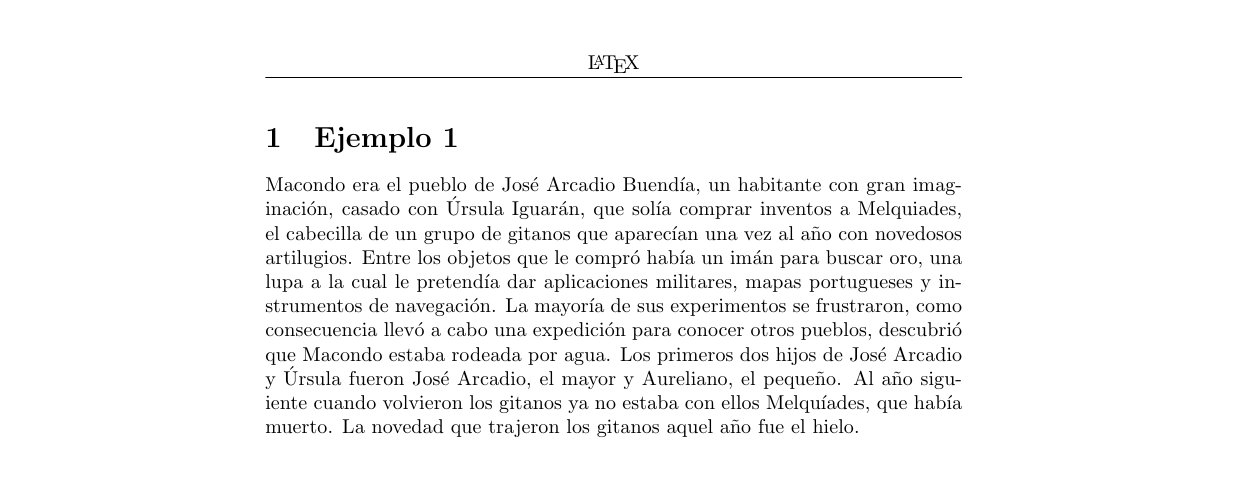
\includegraphics[scale=0.5]{salida1a.png} 
\caption{Cabecera}
\end{figure}
\begin{figure}[H]

\includegraphics[scale=0.5]{salida1b.png} 
\caption{Pie}
\end{figure}
\subsection{Uso}
\begin{lrbox}{\LstBox}
\lstinline+\documentclass[...]{...}+ y \lstinline+\begin{document}+
\end{lrbox}
Para usar el paquete \textbf{fancyhdr} tenemos que cargarlo en el preámbulo\footnote{ espacio entre \usebox{\LstBox}   } como se indica en la línea 2 del código 1.\ref{c1}, luego se empieza a personalizar el encabezado y los pie de páginas usando los comandos  \lstinline+\fancyhead[selectores]{Cabecera}+ y  \lstinline+\fancyfoot[selectores]{Pie}+ para los encabezados y pie de páginas respectivamente, con las opciones\\
\textbf{ Selectores de página}
\begin{lista}
\item E : página par
\item O: página impar
\end{lista}
\textbf{Selectores de campo}
\begin{lista}
\item L: A la izquierda
\item C: Al centro
\item R: A la derecha.
\end{lista}
Los selectores de campo y de página se pueden combinar, por ejemplo de la siguiente manera \lstinline+\fancyfoot[LE,RO]{\thepage}+ , es decir, que el pie de página aparezca a la izquierda en las pares (LE) y a la derecha en las impares (RO). Con \lstinline+\thepage+, decimos que queremos que nos aparezca el número de página. Para que se observe la diferencia entre páginas pares e impares debes colocar la opción global de la siguiente forma \lstinline+\documentclass[...,twoside]{...}+, Es posible que el texto deje de estar centrado por usar twoside, en ese caso hay que usar,\lstinline+\hoffset 0.01cm+ si queremos desplazarlo hacia la derecha un espacio de 0.01cm.\\
Para activar toda esta configuración debemos colocar en la página desde donde queramos que aparezca la configuración \lstinline+\pagestyle{fancy}+, en caso de que queramos que aparezca está configuración en todo el documento lo colocamos en el preámbulo y en la página en particular que no queremos que aparezca \lstinline+\thispagestyle{empty}+.
\subsubsection{Detalles:}
\begin{lista}
\item Si, en mitad del documento, quieres un página sin esto, usas, \lstinline+\thispagestyle{empty}+. 
\item Para limpiar los encabezados y poner otros, \lstinline+\fancyhead{}+ o \lstinline+fancyfoot{}+ o \lstinline+\fancyhf{}+.
\end{lista}
Si en alguna página específica se prefiere aplicar un estilo concreto se puede
usar \lstinline+\thispagestyle{arg}+, donde  \textbf{arg} puede ser:
\begin{lista}
\item fancy si se quiere aplicar el estilo especial
\item plain  que es el estilo por defecto es decir sin encabezado,el  pie de página contiene el número de página centrado
\item empty ninguno estilo es decir sin cabecera ni pie de página.
\item myheadings estilo sin pie de página, el encabezado contiene el número de página y la información suministrada por el usuario
\item headings sin pie de página, el encabezado contiene el nombre del capítulo y sección y / o subsección y número de página.
\end{lista}
En las cabeceras y pies de página también se puede  especificar el
número o nombre del capítulo o sección, etc. Para ello, hay que tener en cuenta que:
\begin{lista}
\item \lstinline+\leftmark+, información de nivel superior (por ejemplo, capítulo en la clase de documento book).
\item \lstinline+ \rightmark+, información de nivel inferior (p.e., sección en clase book).
\end{lista}
Estos comandos se introducen en \lstinline+\fancyhead+ o \lstinline+\fancyfoot+ sugún se requiera, por ejemplo, en un documento clase book, \lstinline+\fancyhead[LO,RE]{\leftmark}+ indica que debe aparecer el nombre del capítulo en la parte izquierda de la cabecera si es página impar, y en la derecha si es página par. Para controlar cómo se representan los capítulos, secciones, etc., en la cabecera o pie de página  del documento, se redefinen los comandos \lstinline+\chaptermark+,\lstinline+\sectionmark+,\lstinline+\subsectionmark+,etc. Antes de colocar \lstinline+\pagestyle{fancy}+ en el documento, por ejemplo:\\
El número de página es \lstinline+\thepage+. Puede aparecer en \lstinline+\fancyhead+ o \lstinline+\fancyfoot+, según se quiera; por ejemplo, \lstinline+\fancyfoot[C]{\thepage}+ indica que el número de página va aparecer centrado en el pie de todas las páginas.
\subsubsection{Lineas de adorno}
Para modificar las lineas de adorno se modifican los comandos \\
% Modifica el ancho de las líneas de cabecera y pie
\lstinline+\renewcommand{\headrulewidth}{0.4pt}+ y\lstinline+\renewcommand{\footrulewidth}{0.4pt}+ para la cabe\-cera y pie de página respectivamente.
%%%%%%%%%%%%%%%%%%%%%%%%%%%%%%%%%%%%%%%%%%%%%%%%
\subsubsection{Avanzado}
Un uso avanzado es por por ejemplo: modificando \lstinline+\chaptermark+,\lstinline+\sectionmark+,\lstinline+\subsectionmark+,etc.\\
redefiniéndolos como:\\
\lstinline+\renewcommand{\chaptermark}[1]{\markboth{\chaptername \thechapter. #1}{}}+
donde:\\
\begin{lista}
\item\lstinline+\chaptername+ = "Chapter" (por defecto) o "Capítulo"  si se ha redefinido tal como se indica en el capítulo() sección (). 
\item \lstinline+\thechapter + = número de capítulo. 
\item Observe  que \lstinline+\thechapter + va  seguido de un punto y \lstinline+#1 + este representa el argumento de \lstinline+\chaptermark+, que es el título del capítulo.
\end{lista}
Aunque el ejemplo es válido para capítulos, se hace de manera análoga para secciones \lstinline+(\sectionmark, \sectionname, \thesection), subsecciones (\subsectionmark, \subsectionname, \thesubsection},+ etc.\\
Es posible omitir alguno de los argumentos anteriores, encerrarlos entre comandos de formateo como \lstinline+\textbf{...}+ o \lstinline+\MakeUpperCase{...}+ (convertir a mayúsculas), etc dentro de los comandos \lstinline+\fancyhead{}+ o \lstinline+fancyfoot{}+.\\

NOTA: Aveces puede ser necesario ampliar el valor de altura de la cabecera \lstinline+(\headheight, por defecto, 12pt)+\lstinline+ o el pie (\footskip, por defecto 30pt)+. Esto nos lo indicará el propio \LaTeX. Para aumentar \lstinline+\headheight+ a 15pt, por ejemplo, puede usarse el comando \lstinline+\setlength{\headheight}{15pt}+ o bien \lstinline+\addtolength{\headheight}{3pt}+. También es posible aumentar o disminuir esta magnitud por un cierto factor; por ejemplo, para un incremento del 125\%: \lstinline+\setlength{\headheight}{1.25\headheight}+.
\\
También se puede cambiar el formato del número de página se establece con \lstinline+\pagenumbering{arg}+, donde arg:
\begin{lista}
\item arabic = números árabes 
\item roman = números romanos en minúscula 
\item Roman = números romanos en mayúsculas 
\item alph = letras en minúscula 
\item Alph = letras en mayúscula.
\end{lista}
Si queremos cambiar por completo las lineas de adorno las podemos redefinir como queramos, por ejemplo de la siguiente forma:
\lstinline+\renewcommand{\headrule}{\vbox to 0pt{\hbox to\headwidth{\color{gris}{\dotfill}}\vss}}+ 
Ejemplo completo\\
\begin{source}[Lineas de adorno]{c2}
\def\dayinmonth#1{%
  \ifcase#1 31\or28\or31\or30\or31\or30
            \or31\or31\or30\or31\or30\or31\fi}
\newcommand{\Today}[1][0]{%
  \advance\day by #1
  \edef\DiM{\dayinmonth{\the\month}}
  \ifnum\day>\DiM 
    \day=\numexpr \the\day-\DiM\relax 
    \advance\month\@ne
  \fi  
  \today}
\usepackage{advdate}\newcommand{\parcial}[2]{#1\, #2}
\newcommand{\porcentaje}[1]{#1\%  }
\newcommand{\materia}[1]{#1}
\newcommand{\fecha}[1]{\DayAfter[#1]}
\newcommand{\logom}[5]{\setlength{\unitlength}{1mm}
\begin{picture}(150,30)
\put(5,8){\includegraphics[width=0.2\textwidth]{/home/antalcides/.lyx/templates/LOGO1.jpg}} \put(60,15){\bf DIVISI\'ON DE
CIENCIAS B\'ASICAS} \put(60,10){\bf DEPARTAMENTO DE MATEM\'ATICAS Y
ESTAD\'ISTICA} \put(60,5){\bf \parcial{#1}{#2} \, DE \, \materia{#3\, (\porcentaje{#4})}} \put(5,0){\bf
NOMBRE:\hspace{115mm} \DayAfter[#5]}
\end{picture}}\newcommand{\logopie}{\vspace{10pt}
\begin{minipage}{0.3\textwidth}
\includegraphics[width=0.2\textwidth]{direcci\'on de la imagen}
\end{minipage}\hspace*{5mm}
\begin{minipage}{0.7\textwidth}
\bf \small Prohibido el uso de cualquier dispositivo electr\'onico con c\'amara o conexi\'on a internet y el  prest\'amo de calculadora o cualquier otro material permitido
\end{minipage}}
\fancyhf{} \clearpage
\fancyhead[C]{}
\fancyfoot{\logopie}
\end{source}
Obteniendo la salida \\
\begin{figure}[H]
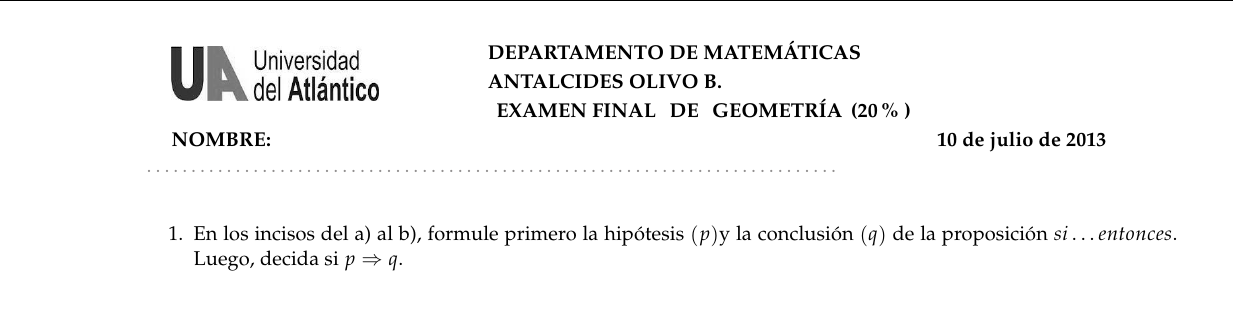
\includegraphics[scale=0.5]{cabecera1.png} 
\caption{Cabecera de examen}
\end{figure}
\begin{figure}[H]
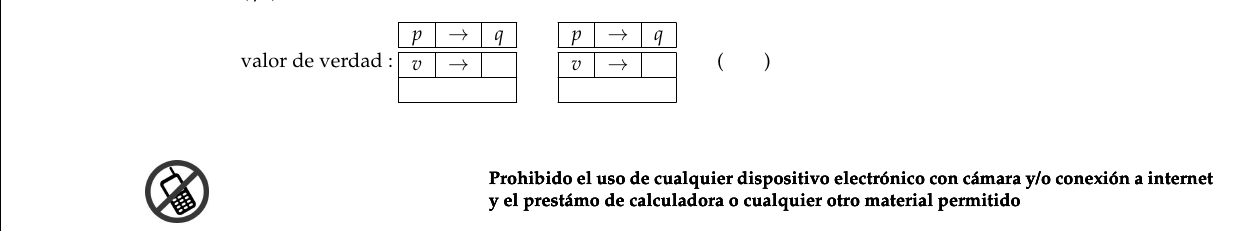
\includegraphics[scale=0.5]{pie1.png} 
\caption{Pie de examen}
\end{figure}
\begin{source}[Taller]{c4}
\renewcommand{\headrule}{
\begin{minipage}{1\textwidth}
\hrule width \hsize \kern 1mm \hrule width \hsize height 2pt 
\end{minipage}}
\renewcommand\footrule{\begin{minipage}{1\textwidth}
\hrule width \hsize height 2pt \kern 1mm \hrule width \hsize   
\end{minipage}\par}
\end{source}
\begin{figure}[H]
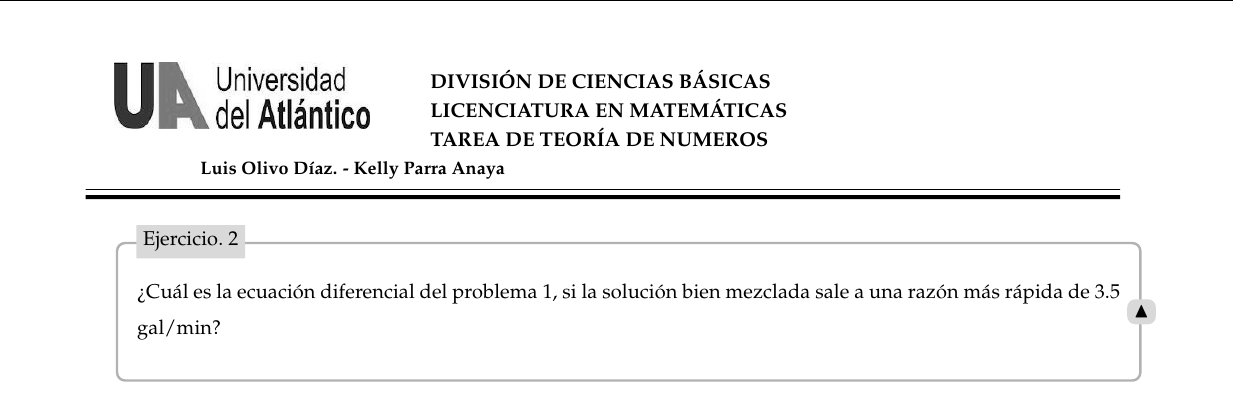
\includegraphics[scale=0.5]{cabecera2.png} 
\caption{Cabecera de tarea}
\end{figure}
%%%%%%%%%%%%%%%%%%%%%%%%%%%%%%%%%%%%%%%%%%%%
\begin{source}[Ejemplo completo]{c3}
\documentclass[...,twoside,...]{book} % Documento de clase book a dos caras
...
\usepackage{fancyhdr}
...
\pagestyle{fancy}
\fancyhf{}
\fancyhead[LO]{\leftmark} % En las p\'aginas impares, parte izquierda del encabezado, aparecer\'a el nombre de cap\'itulo
\fancyhead[RE]{\rightmark} % En las p\'aginas pares, parte derecha del encabezado, aparecer\'a el nombre de secci\'on
\fancyhead[RO,LE]{\thepage} % N\'umeros de p\'agina en las esquinas de los encabezados
\renewcommand{\chaptermark}[1]{\markboth{\textbf{\thechapter. #1}}{}} % Formato para el cap\'itulo: N. Nombre
\renewcommand{\sectionmark}[1]{\markright{\textbf{\thesection. #1}}} % Formato para la secci\'on: N.M. Nombre

\renewcommand{\headrulewidth}{0.6pt} % Ancho de la l\'inea horizontal bajo el encabezado
\renewcommand{\footrulewidth}{0.6pt} % Ancho de la l\'inea horizontal sobre el pie (que en este ejemplo est\'a vac\'io)
\setlength{\headheight}{1.5\headheight} % Aumenta la altura del encabezado en una vez y media
...
\begin{document}
... 

\end{source}
\backmatter
%
\begin{thebibliography}{99}
\addcontentsline{toc}{chapter}{\numberline{}\bibname}
\ifx\pdfoutput\undefined % No se est'a ejecutando pdftex
\else
\pdfbookmark{\bibname}{bibliografia}
\fi

\bibitem{manual} Leslie Lamport.  \newblock \emph{{\LaTeX:} A Document
    Preparation System}.  \newblock Addison-Wesley, Reading,
  Massachusetts, segunda edici'on, 1994, ISBN~0-201-52983-1.

\bibitem{texbook} Donald~E. Knuth.  \newblock \textit{The \TeX{}book,}
  Tomo~A de \textit{Computers and Typesetting}, Addison-Wesley
  Publishing Company (1984), ISBN~0-201-13448-9.

\bibitem{companion} Michel Goossens, Frank Mittelbach and Alexander
  Samarin.  \newblock \emph{The {\LaTeX} Companion}.  \newblock
  Addison-Wesley, Reading, Massachusetts, 1994, ISBN~0-201-54199-8.
 
\bibitem{local} Cada instalaci'on de  \LaTeX{} deber'ia proporcionar
  la llamada \emph{Gu'ia Local de \LaTeX}, que explica las cosas que
  son particulares del sistema local. Deber'ia residir en un fichero
  llamado \texttt{local.tex}. Por desgracia, en algunos sitios no se
  halla dicha gu'ia. En este caso, p'idale ayuda a un experto de
  \LaTeX.
 
\bibitem{usrguide} \LaTeX3 Project Team.  \newblock \emph{\LaTeXe~for
    authors}.  \newblock Viene con la distribuci'on de \LaTeXe{} como
  \texttt{usrguide.tex}.

\bibitem{clsguide} \LaTeX3 Project Team.  \newblock \emph{\LaTeXe~for
    Class and Package writers}.  \newblock Viene con la distribuci'on
    de \LaTeXe{} como \texttt{clsguide.tex}.

\bibitem{fntguide} \LaTeX3 Project Team.  \newblock \emph{\LaTeXe~Font
    selection}.  \newblock Se incluye en la distribuci'on de \LaTeXe{}
    como \texttt{fntguide.tex}.

\bibitem{graphics} D.~P.~Carlisle.  \newblock \emph{Packages in the
    `graphics'\ bundle}.  \newblock Se incluye en el conjunto `graphics'\
  como \texttt{grfguide.tex}, disponible en el mismo sitio de donde se
  ha tomado la distribuci'on de \LaTeX.
\end{thebibliography}


 \end{document}
 
 
